\documentclass[english,version-2019-11]{uzl-thesis}
% Copy this file as a template for your thesis. You will have to take
% action at all places marked by
%
% !!!!!!!!!!!!!!!!!!!!!!!!!!!!!!!!!!
% !!! Your action is needed here !!!
% !!!!!!!!!!!!!!!!!!!!!!!!!!!!!!!!!!
%
% The first place your action is needed is the first line of this
% document:
%
%
% Language of the thesis:
%
% You must use either 'german' or 'english' above, depending on the
% language used in the main text. This will automatically setup a lot
% of things in the background.
%
%
% Version of the class:
%
% You must specify which version of the thesis class is to be
% used. This is important in case the class style changes in later
% years, but we still want an older thesis to look the same, even when
% things are changed in the class.
%
% Do not change or remove the version-xxxx key.
%
%
% Text encoding:
%
% Your thesis *must* be encoded in utf8 (unicode), which is the
% default in most editors these days. Do *not* change this to latin8.
%%%
%
% Main setup:
%
%%%
%
% You must use the \UzLThesisSetup command to specify numerous things
% about your thesis. This includes the entries on the title page, the 
% abstracts, and the bibliography style. You do so by specifying
% so-called "values" for so-called "keys". For instance, 
% for the key "Autor" you must provide your name as the value. You do
% so by writing 'Autor = {Max Mustermann}', that is, the value is put
% into curly braces. You can use the \UzLThesisSetup command
% repeatedly and the order in which you provide the keys is not
% important. 
%
% Everything shown on the title page must be in German -- even
% if the thesis is written in English! Just insert German text for
% German keys and English text for English keys (like 'Abstract' needs
% English text, while 'Zusammenfassung' needs German text).

\UzLThesisSetup{
  %
  % First, specify the institut or clinic at which the thesis was
  % written. You get the logo file from them (make sure it has the
  % correct size, namely the same as the example). If they do not have
  % a logo, the university's default logo is used.
  %
  % The 'verfasst' gets two arguments. Change the first to {an der}
  % for clinics, as in 'Verfasst = {an der}{Medizinischen Klinik I}'
  %
  Logo-Dateiname        = {uzl-thesis-logo-itcs.pdf},
  Verfasst              = {am}{Institut f{\"u}r Informationssysteme},
  %
  % The titles:
  %
  Titel auf Deutsch     = {
    Rahmenwerk f{\"u}r die Simulation von verteilter Datenbankanfrageverarbeitung
    im semantischen~Internet~der~Dinge
  }, 
  Titel auf Englisch    = {
    Simulation Framework for Distributed Database Query Processing
    in the Semantic~Internet~of~Things 
  },
  %
  % Author and supervisor:
  % 
  % Note that the 'Betreuer' or 'Betreuerin' is the supervisor, that
  % is, the professor who officially supervises the thesis. If there
  % is also an assistent of the professor who helped (typically a
  % lot), use 'Mit Unterstützung von' to thank that person. If the
  % thesis was mainly written 'externally' at some company or another
  % institute, point this out using 'Weitere Unterstützung'. 
  % 
  % For your own name, do *not* add things like "BSc" or "BSc
  % cand.". For the supervisor, you should normally include
  % "Prof. Dr." or "PD Dr." (ask your supervisor, what is
  % appropriate), but nothing more (so no
  % "Univ.-Prof. Dr. Dr. h.c. mult." unless your supervisor insists).  
  %
  Autor                 = {Johann Mantler},
  Betreuer            = {Prof. Dr. rer. nat. habil. Sven Groppe},
  % 
  % Optional: Supporting persons and institutions. The text should be
  % in German, even for an English thesis.
  %
  Mit Unterstützung von = {Benjamin Warnke},
  % 
  %   Weitere Unterstützung = {
  %     Die Arbeit ist im Rahmen einer Tätigkeit bei der Firma Muster GmbH
  %     entstanden.
  %   },
  %
  %
  % Your Degree Programm (Studiengang)
  %
  % Specify 'Bachelorarbeit' or 'Masterarbeit' and the degree
  % programme. Make sure the name of programme is correct and not
  % some abbreviation or some incorrect variant. For instance:
  % 'Medizinische Ingenierwissenschaft', but not 'MIW';
  % 'Medizinische Informatik', but not 'Medizin-Informatik';
  % 'Informatik', but not 'Informatik (SSE)'.
  %
  % Use German names for German programmes and English names for
  % English ones, so 'Infection Biology', not 'Infektionsbiologie'. 
  % For programmes that have a German bachelor and an English master,
  % use the German name for a bachelor thesis and the English name for
  % the master thesis.
  %
  Masterarbeit,
  Studiengang           = {Entrepreneurship in digitalen Technologien},
  %
  % Date on which the thesis is turned in:
  %
  Datum                 = {26. Juli 2021},
  %
  % The English abstract. You must always provide abstracts in German
  % and in English. 
  %
  Abstract              = {
    The growing computing capacities of small devices in the Internet of Things (IoT) have led to the edge computing paradigm. More and more things on the edge of the Internet can not only generate data, but also save and process it. One way of using this computing capacity are distributed database management systems (DBMS) that are adapted to the IoT platform. The DBMS instances run on the edge devices and cooperate for query processing. For the development and evaluation of such DBMSs, we present a new simulator with which modeled instances of a real existing DBMS can be simulated in a configurable edge computing environment without virtualization. Furthermore, we present a new protocol for distributed query processing, in which the operator graph is mapped to the routing tree of an IoT routing protocol and calculated in a distributed manner. The aim of the protocol is to reduce resource consumption by executing operators (e.g. joins, filters) as early as possible. Both contributions are evaluated with the Semantic Web DBMS LUPOSDATE3000 in a modeled example scenario.
  },
  Zusammenfassung       = {
     Die wachsenden Rechenkapazit{\"a}ten kleiner Ger{\"a}te im Internet der Dinge (IoT) haben zum Edge-Computing-Paradigma gef{\"u}hrt. Immer mehr Dinge am Rand des Internets k{\"o}nnen Daten nicht nur generieren, sondern auch speichern und verarbeiten. Eine M{\"o}glichkeit diese Rechenkapazit{\"a}ten zu nutzen ist die Verwendung von verteilten Datenbankmanagementsystemen (DBMS), welche an die IoT-Plattform angepasst sind. Die DBMS Instanzen laufen auf den Edge-Ger{\"a}ten und kooperieren bei der Anfrageverarbeitung. F{\"u}r die Entwicklung und Evaluation solcher DBMS pr{\"a}sentieren wir einen neuen Simulator, mit dem modellierte Instanzen eines real existierenden DBMS in einer konfigurierbaren Edge-Computing-Umgebung ohne Virtualisierung simuliert werden k{\"o}nnen. Weiterhin pr{\"a}sentieren wir ein neues Protokoll f{\"u}r die verteilte Anfrageverarbeitung, bei dem der Operatorgraph auf den Routing-Baum eines IoT-Routing-Protokolls abgebildet und verteilt berechnet wird. Das Ziel des Protokolls ist, den Ressourcenverbrauch durch eine m{\"o}glichst fr{\"u}he Ausf{\"u}hrung von Operatoren (z.B. Joins, Filter) zu senken. Beide Beitr{\"a}ge werden mit dem Semantic Web DBMS LUPOSDATE3000 in einem modellierten Beispielszenario evaluiert.
  },
  %
  % Optional: 'Danksagungen' (German) or 'Acknowledgements'
  % (English). Both keys are optional and both have the same effect of
  % adding an acknowledgements text after the abstracts and before the
  % table of contents.
  %
  %Acknowledgements      = {
  %  TODO 
  %},
  % Bibliography style: Choose between
  % 
  % 'Alphabetische Bibliographie'
  % for all degree programmes in the natural sciences 
  % 
  % 'Numerische Bibliographie'
  % alternative for all other degree programmes
  % 
  % Either will load biblatex and setup the citation methods and the
  % bibliography styles correctly. You should not mess with them.
  % 
  %Alphabetische Bibliographie
  % Alternatively:
   Numerische Bibliographie
}

% Technical note: All styling is done via the command
%
% \UzLStyle{...}
%
% where ... is a key-value list just as for \UzLThesisSetup. The
% difference is just that everything having to do with styling as
% controlled by \UzLStyle, while the more “formal” setup keys are
% controlled by \UzLThesisSetup.
%

%\UzLStyle{alegrya modern design}
\UzLStyle{computer modern basic design}




%%%%%%%%
%
% Now, include the package you need here using \usepackage. 
%
% However, many standard packages are already loaded by the class:
%
% amsmath, amssymb, amsthm, babel, biblatex, csquotes, etoolbox,
% filecontents, fontspec, geometry, hyperref, tikz (with libraries
% arrows.meta, positioning and shapes), varioref, url 
%
% Indeed, in many cases you will not need any extra packages.
%
%%%%%%%
\usepackage{multirow}
\usepackage{csquotes}
\usepackage{graphicx} 
\usepackage{tikz}
\usepackage[export]{adjustbox}
\usepackage{booktabs}
\usepackage{indentfirst}

\begin{document}
\uzldeflanguageshorthand{SPARQL}{style=code,language=SPARQL}

\chapter{Introduction}
With the progressive downsizing of computers and the rapid evolution of
the Internet, the \emph{Internet of Things} (IoT) was established~\cite{AndreasTeubler}.
While in the classic Internet humans generate information that can 
be read and processed by other humans, in the IoT the things
are generating and possibly processing information~\cite{AITScript}.
Things are physical objects enhanced with appropriate electronics
such as sensors or actuators. With sensors, things can perceive
their environment and with actuators make changes in it.
Equipped with means of communication, things can connect to other things
or even larger computers via a network such as the Internet and
act together. On this basis, innovative applications can be developed
for various problem domains that have a lasting impact on our society.
The spectrum of IoT encompasses both simpler applications in the home
with a few things and more complex applications in the city with many
thousands of things. Examples of applications in the home are smart coffee machines or robotic vacuum cleaners, which control
themselves based on information from the Internet or are remotely
controlled via the Internet~\cite{AndreasTeubler}. Examples of applications in the city are
bluetooth beacons distributed along the roadside that communicate
with a smartphone app of a visually impaired user in order to safely
navigate them to their destination.

The need for IoT applications is evident in the enormous number of things
in the environment. 
The estimates widely used in the literature range from
24~\cite{RoutingIssuesSurvey} to 50~\cite{IoTEvolution} or 100~\cite{SimChallenges} billion things by 2020. 
While the amount of data
produced by sensors in the home remains manageable,
very large amounts of data can accumulate in complex IoT applications.
IoT is considered to be an essential driver for Big Data~\cite{IoTSim}. 
Cloud computing alone is no longer sufficient as a data sink
and place of data processing. New approaches such as fog and edge computing
have emerged, which can be scaled better with the enormous number of things.
More powerful things like smartphones can, for example, preprocess
data and provide initial interim results as well as
relieve the communication path to the cloud.
In addition to managing the amount of data, the semantic use of this data
is also a challenge. With the help of ontologies, applications can infer
the semantics of the data and act accordingly. The realization of such
IoT systems with numerous interconnected things requires further research
activity with regard to infrastructure, data storage and query as well
as semantic enrichment of the data.

The research project \emph{Big Data Management for the Semantic Internet of Things} (BigSIoT) was launched at the University of L{\"u}beck from the 
\emph{Institute of Information Systems} (IFIS) together with the \emph{Institute of Telematics} (ITM) to address the above-mentioned challenges.
One possible solution to this challenges
is a distributed semantic web \emph{database management system} (DBMS) that can serve as the backbone for IoT applications. Instances of the database management system could run on the more powerful things to distribute the data storage and processing.
IFIS has already developed a centralized semantic web DBMS called LUPOSDATE3000~\cite{Warnke21Flexible}. As part of the research project, this DBMS is now being implemented as a distributed DBMS that supports the IoT platform.
For this, among other things, a protocol for distributed query processing in the IoT must be developed and evaluated.

In this master's thesis, we design and develop a simulation framework that can be used by distributed DBMSs such as LUPOSDATE3000 to simulate the IoT environment.
In addition, a protocol for distributed query processing is designed and tested in the simulation.

\section{Contributions of this Thesis}
The first contribution of this thesis is the development of a new event-driven simulator with which real, distributed DBMSs can be tested in a simulated edge computing environment. According to a comparative study of already published IoT simulators, this simulator is the first to enable direct integration of a real DBMS without virtualization. By exchanging the real database states of the DBMS instances at defined times, thousands of instances can be simulated. There is also a modeling and simulation of the \emph{Routing Protocol for Low-Power and Lossy Networks} (RPL) to provide multi-hop routing of network packets in a configurable IoT topology. The payload of the packets is real data that can be stored in the databases. The simulator is designed as a framework that can control a DBMS via a well-defined interface. In addition, the event-driven core of the simulator was developed as an independent and self-contained module. This module is universally applicable and can be used in other work to build new simulators. The implementation is in the programming language Kotlin to support different platforms like JavaScript, \emph{Java Virtual Machine} (JVM) and native binaries. The usability of the simulator was checked with the Semantic Web DBMS LUPOSDATE3000. A performance evaluation has shown that 1170 instances of this system can be started in a JVM with a heap size of 2048 megabytes.

The second contribution of this thesis is the design of a novel query processing protocol for distributed DBMS in an edge computing environment. The operator graph of a query is mapped to the routing tree of an IoT routing protocol and calculated in a distributed manner. The goal is to minimize the network load by calculating operators as close as possible to the data sources. The protocol design describes two phases with the respective communication steps, the message types and the cooperation with a routing protocol. A generic protocol interface for DBMS instances is also provided. The subtleties of the protocol implementation are left to the DBMS to analyze different variants. The interface as well as the universal parts of the protocol are implemented in the simulator. In a modeled parking space finder scenario, the performance of the protocol in terms of resource consumption is evaluated. The evaluation has shown that the current implementation in LUPOSDATE3000 is not yet sufficient to replace the centralized query processing in the IoT. An analysis of this identifies the sensor data distribution strategy between the LUPOSDATE3000 instances as a problem. The analysis also shows how LUPOSDATE3000 has to perform so that the distributed query processing is more resource-efficient than the centralized variant.


\section{Structure of this Thesis}
The remainder of this thesis is organized as follows: First, Chapter~\ref{chapter_Basics} introduces the necessary basics such as IoT, computing paradigms, routing, query processing and simulation. This chapter ends with a list of related work on simulators and distributed query processing in the edge computing environment. Chapter~\ref{chapter_Concept} starts with a detailed problem definition of this thesis as well as the motivation for a distributed query processing protocol in edge computing. Then the concept for the simulator with a modeling of the IoT environment is presented. Afterwards, different approaches for the protocol are discussed and finally one solution is presented.
Chapter~\ref{chapter_Implementation} describes the most important parts of the simulator implementation. This also includes the interface
to DBMSs for protocol usage. In Chapter~\ref{chapter_Evaluation} the implementation is evaluated. A general performance analysis of the simulator is carried out with and without LUPOSDATE3000. The next step is the analysis of the distributed query processing using an example scenario with different queries. Finally, the thesis ends in Chapter~\ref{chapter_Conclusion} with a summary and discussion of future work.

\chapter{Basics}
\label{chapter_Basics}
Overall, this thesis is interdisciplinary in the fields of IoT, database systems and simulation. The necessary basics are briefly presented in this order. The related work is presented at the end of this chapter.

\section{Internet of Things}
IoT can be seen as an extension of the Internet, where
the Internet is extended by adding things as network
nodes. The point is to connect the physical objects
that are not yet connected with the help of the Internet
and thus create significant added value~\cite{BookCisco}. The added
value is a better collaboration between
humans and machines through new types of applications
in various areas. Application domain names often
begin with the prefix "Smart" (Smart City, Smart Healthcare,
Smart Farming, Smart Factory, etc.).
The Cisco \emph{Internet Business Solutions Group} (IBSG)
defines the birth of the IoT as 
\emph{\enquote{simply the point in time when more things or
objects were connected to the Internet than people.}}~\cite{IoTEvolution}
In other words, when the number of connected devices
per person is more than $1$. They date the year
of birth to 2008.
Instead of counting the number of people on the Internet,
the world population is used as a reliable upper limit.
The figure ~\ref{figure_iot_birth} shows the course.
\begin{figure}[htpb]
  \centering
  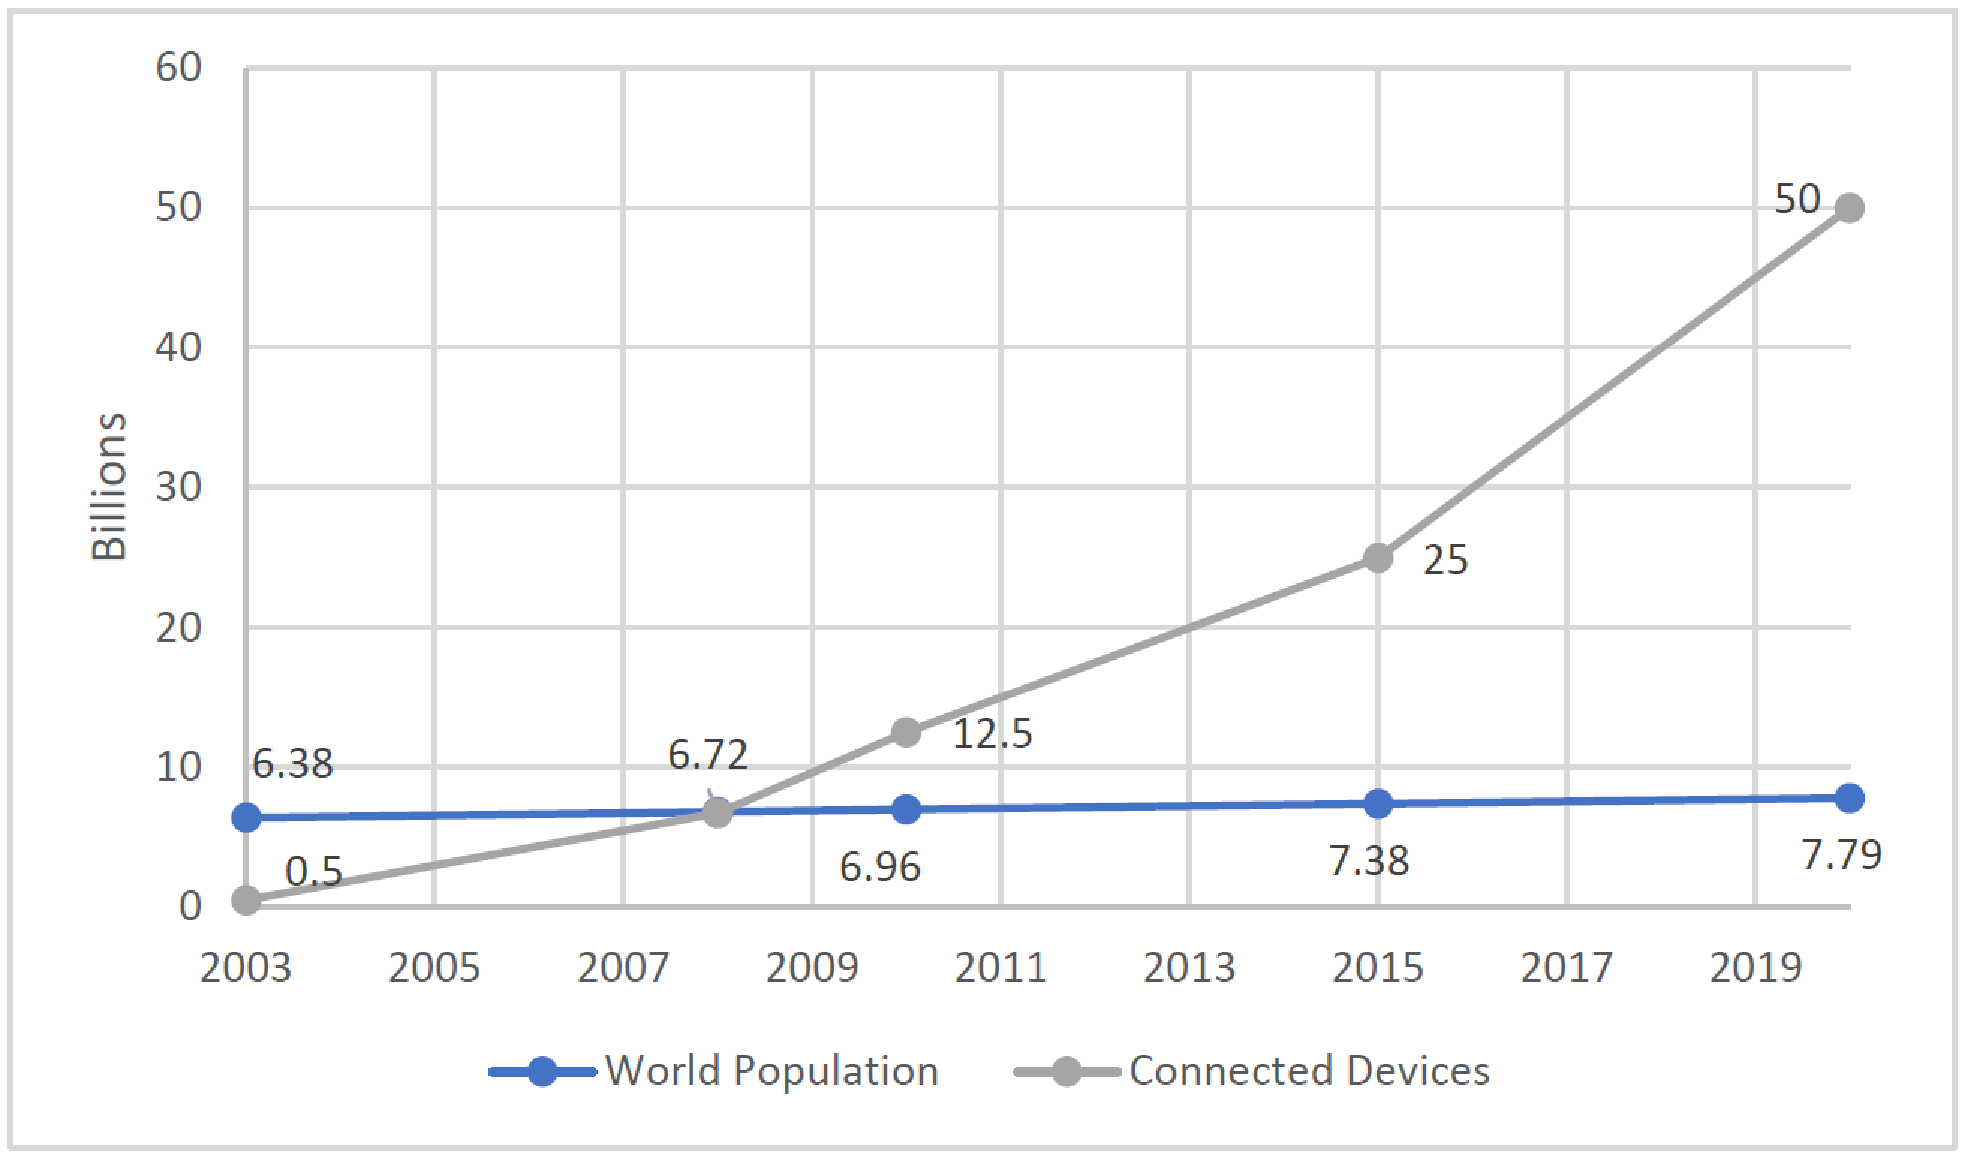
\includegraphics[scale=0.4]{figure_iot_birth.pdf}
  \caption{According to Cisco IBSG, the age of the IoT emerged between 2008 and 2009. Data of connected devices is from~\cite{IoTEvolution} and data of world population is from~\cite{WorldPopulation}.}
  \label{figure_iot_birth}
\end{figure}
In addition to this definition that emphasizes
the temporal aspect, there are many other
definitions that illuminate other aspects.
Dhumane et al. list some notable definitions in their survey paper~\cite{RoutingIssuesSurvey}.

An in-depth definition that emphasizes the inclusion of things
on the Internet is:
\emph{\enquote{The
semantic origin of the expression is composed of two words
and concepts: Internet and Thing, where Internet can be
defined as the world-wide network of interconnected
computer networks, based on standard communication
protocol, the Internet suite (TCP/IP), while Thing is an
object not precisely identifiable. Therefore semantically,
Internet of Things means the world wide network of interconnected
objects uniquely addressable, based on
standard communication protocols.}}~\cite{EuropeanCommission}

One definition that highlights the desired goals of the IoT is:
\emph{\enquote{IoT allows people and things to be connected
Anytime, Anyplace, Anything and Anyone ideally using any
path/network and Any service.}}~\cite{StrategicRoadmap}


\subsection{Constrained Devices}
Characteristic of the IoT are the things that differ
from traditional computers on the Internet.
One difference is that things are embedded in the environment
of everyday life and are therefore ubiquitous.
This fact leads directly to the next difference that things
have limited or very limited computing resources.
The \emph{Request for Comments} (RFC) informational publication 7228 uses the term constrained devices~\cite{rfc7228}.
To a certain extent, the constrained devices can use their
resources to act smartly by communicating with
other things and computers. For this reason,
the term smart objects is also used in the literature~\cite{BookCisco}.
Below is a list of typical properties:
\begin{itemize}
\item Things have
some sort of processing unit to compute data.
The performance varies, but remains mainly in the lower
performance spectrum. The spectrum ranges, for example,
from 8-bit single-board computers to high-end phones and tablets.
The latter no longer count as constrained devices~\cite{rfc7228}, but as things in the IoT~\cite{BookCisco}.
\item On the other hand, there are also simpler things like
\emph{Radio Frequency Identification} (RFID) chips that can only be programmed
to a very limited extent~\cite{Tanenbaum}.
\item Just like the hardware,
the software also varies, which leads to maximum
heterogeneity in the network.
\item In order to perceive
and influence the environment, things can have
sensors and actuators, but do not have to.
\item In any case, things have some kind of means of
communication. Data is usually transmitted
wirelessly, but cabling is also possible.
\item For electronics, a power supply is required,
which can be implemented, for example,
via a battery or, more rarely, via a permanent
connection to the power grid. This means that things
can also fail due to a lack of energy and must
therefore use the available energy sparingly.
Some things can therefore also go to sleep and
only become active again when needed~\cite{TinyDB}.
\item Things
with a permanent power connection are usually stationary,
while battery-operated things can be partially
mobile or highly mobile. A good example of a highly
mobile thing is an intelligent vehicle that moves quickly
on the road and participates in Internet traffic
via mobile communications.
 \end{itemize}

\subsection{Constrained Networks}
Things can be individually connected to the Internet.
Or they form a network with other things,
which is then connected to the Internet via a gateway.
In the terminology of RFC 7228, things on the network are
called constrained nodes, and a network with constrained nodes
is called a constrained network~\cite{rfc7228}.
Constrained networks are usually on the edge of the Internet,
which means no Internet traffic flows through them~\cite{AndreasTeubler}.
The prerequisite for the connection of the constrained
nodes to the Internet is the implementation
of a TCP/IP stack on these nodes. Alternatively,
a gateway can implement a network stack for the nodes.
In any case, the \emph{Internet Protocol} (IP) must be understood,
as it forms the narrow waistline of the Internet
as the core protocol~\cite{smallWaist}. New protocols for constrained networks can then be implemented above or below IP.
Due to the enormous number of Internet addresses required in IoT,
only IPv6 can be used. The addresses in IPv4 are already exhausted
or almost exhausted. IPv4 currently only holds up thanks to special techniques such as \emph{network address translation} (NAT), which have a negative impact on the architecture of the Internet.~\cite{Kurose}.

A related term to constrained networks is \emph{Low-Power and Lossy Networks} (LLN).
An LLN is also a constrained network, but with certain characteristics that further restrict network use~\cite{rfc7228}. Characteristic properties are packet losses, variance in the data rate and poor stability of the connections~\cite{rfc7228}. However, the terms cannot be clearly separated from one another.



\subsection{Wireless Sensor Networks}
A \emph{Wireless Sensor Network} (WSN) is an example of a constrained network.
Many things, mostly just called sensors in this context,
are scattered in an environment in order to observe a feature of interest in it.
Each sensor takes a sample from its location at periodic intervals, when a certain event occurs or on request. The samples can be saved directly on the sensor device.
Then the sensor can send its samples on request.
Often, however, sensor devices are very limited and therefore send their samples on to a data sink.
This results in a continuous stream of data from
many sources to a sink~\cite{BookCisco}.
Depending on the application, the nodes in a WSN can also be equipped with actuators in order to influence their environment. A WSN with many nodes that have both sensors and actuators is also known as a \emph{Wireless Sensor and Actuator Network} (WSAN)~\cite{BookCisco}.
WSNs and WSANs are multi-hop ad-hoc networks. The nodes connect to each other autonomously and also react spontaneously to changes in the topology~\cite{BookCisco}. For this purpose, nodes can hold several alternative connections.

\subsection{Protocols in Constrained Networks}
The IoT is about connecting things to the internet. For this purpose, constrained nodes need protocols from the Internet layer upwards that are compatible with the protocols of unconstrained nodes. Only protocols in the link layer remain completely different. Low-power Wi-Fi or 802.15.4 of \emph{Institute of Electrical and Electronics Engineers} (IEEE) are often used for the link layer~\cite{rfc7102}.

An additional adaptation layer is required to bring IEEE 802.15.4 devices to the Internet. A full IPv6 packet does not fit in an IEEE 802.15.4 frame. The minimum packet size of IPv6 that can be transmitted in a frame in the link layer is 1280 bytes. If the possible payload of a link layer frame is smaller, a fragmentation and reassembly mechanism must be implemented below IP. The payload of the IEEE 802.15.4 frame has only 127 bytes available. Fragmentation must therefore be carried out using an adaptation layer that lies between IPv6 and IEEE 802.15.4. In addition, IPv6 headers are compressed to create even more space for the payload within the available 127 bytes.
This adaptation layer is called \emph{IPv6 over Low-Power Wireless Personal Area Network} (6LoWPAN). In 6LowPAN networks, \emph{User Datagram Protocol} (UDP) is used in the transport layer. The UDP header is also compressed.~\cite{rfc4944}

RPL is the established standard for the destination-oriented sending of IPv6 packets across several hops~\cite{RPLApplications}. RPL is a variant of the distance vector algorithm that is optimized for constrained nodes.

In addition, if there are sufficient resources, an application protocol can be used. For example, \emph{Constrained Application Protocol} (CoAP) can bring constrained nodes to the web. CoAP is a lightweight alternative to \emph{Hypertext Transfer Protocol} (HTTP) that provides a subset of the HTTP methods (GET, PUT, POST and DELETE)~\cite{SemanticModels}. It is designed in such a way that interaction with HTTP is possible (HTTP-CoAP proxying)~\cite{rfc7252}. Constrained nodes such as sensors could, for example, act as web servers and deliver their data with a GET request (e.g., http://ipv6-address-or-dns-name/sensor)~\cite{SemanticModels}. Figure~\ref{figure_wsn} illustrates a possible CoAP protocol stack in a WSN. The linking between the 6LowPAN network and another network takes place via a gateway device. For example, a web application from another network can query the sensors in the WSN.
\begin{figure}[htpb]
  \centering
  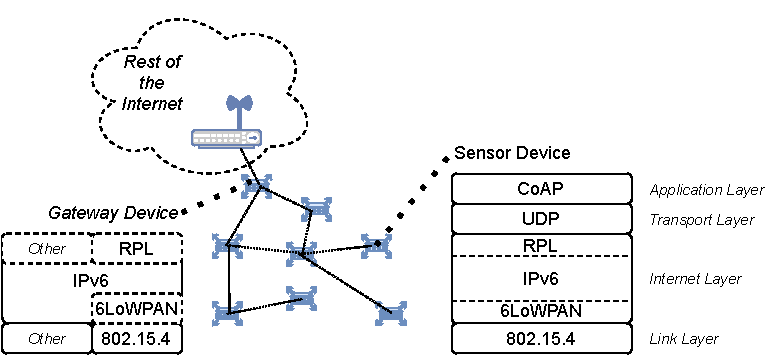
\includegraphics{figure_wsn.pdf}
  \caption{Example of a WSN.}
  \label{figure_wsn}
\end{figure}


\section{Semantic Internet of Things}
The World Wide Web as the largest application service on the Internet is geared towards humans as end users~\cite{SWPaper}. Humans can easily understand information on web pages. Despite heterogeneity on several levels (e.g. structure of the page, language, character coding), the data is recognized and linked to information in order to decipher the semantics~\cite{SWBookHitzler}. Applications cannot easily understand the semantics of the data.
In order to automatically recognize the semantics, methods for the automatic processing of knowledge must be used.

The term Semantic Web covers a whole bundle of formal languages for knowledge processing on the web. The languages are standardized by the \emph{World Wide Web Consortium} (W3C) and enable knowledge processing across application boundaries. That means that one web application can understand the semantics of the data of another web application, even though both applications were developed independently of one another. The interaction between heterogeneous applications can take place by homogenizing the data. The Semantic Web can be seen as an extension of the Web that enables better cooperation between people and their applications, in that the existing data on the Web is given a well-defined semantics that can be understood by applications~\cite{SWPaper}.

With the advent of IoT, the Semantic Web has gained in importance. Things (machines) come to the fore as producers and consumers of data. With the help of semantically enriched data, things can communicate with each other more effectively and act inferentially. Using application protocols such as CoAP, things can appear directly on the web and thus participate in the Semantic Web~\cite{WoT}. In this context, the Semantic Web is also referred to as the Semantic Web of Things~\cite{WoT}.

The semantic technologies that characterize the Semantic Web are not limited to the Web. Rather, they can be used universally. In addition, things don't necessarily have to be on the Web either. The Web is just one possible application service among many. The term Semantic Internet of Things is more universal and generally stands for the use of semantic technologies in the IoT.
\subsection{Semantic Technologies}
As a basic data format, a formal language is needed that can represent data in a linked manner. Data formats with tree structures as offered by the \emph{extensible markup language} (XML) are not sufficient~\cite{SWBookHitzler}. A graph structure is required for the data format~\cite{SWBookHitzler}. The language \emph{Resource Description Framework} (RDF) has prevailed. RDF is standardized by the W3C and forms the core language of the Semantic Web.

RDF uses triples in the sense of $(subject, predicate, object)$ and is thus based on a simple natural language sentence structure. $Subject$ represents a resource, $Predicate$ a property and $Object$ a value of the property~\cite{SWBook}. For example, with the sentence: \enquote{A sensor observes a place}, the \enquote{sensor} is the subject, \enquote{observes} is the predicate and \enquote{place} is the object. In RDF, \emph{internationalized resource identifiers} (IRIs) are used for uniqueness when naming resources. There are several notations for the representation of the triples. Listing~\ref{listing_simple_triple} shows the example sentence as triple in N3 notation.
\begin{SPARQL}[caption={A simple example of an RDF triple in N3 notation.},
  float, label=listing_simple_triple, morekeywords={@prefix}, captionpos=b]
@prefix p: <http://domain/> .
p:sensor p:observes p:place .

# alternative:
# <http://domain/sensor> <http://domain/observes> <http://domain/place> .
\end{SPARQL}

The IRIs do not have to be a valid web address. They serve primarily as unique identifiers. This uniqueness allows resources to be linked. Listing~\ref{listing_linked_triple} shows $3$ linked triples. By linking, it can be concluded that $smartphoneX$ has a sensor that is observing $place_1$. With a few triples, the semantics are of little use. But with the amount of linked resources, the semantic interpretation possibilities for each individual resource also increase. The IRIs can be freely assigned. However, in order to seamlessly link resources across system boundaries, it is necessary to agree on the use of the same IRIs. A set of well-defined IRIs is called a vocabulary~\cite{SWBookHitzler}. If data systems are based on standardized vocabularies, data exchange without conversion is possible.
\begin{SPARQL}[caption={A simple example of linking triples using IRIs.},
  float, label=listing_linked_triple, morekeywords={@prefix}, captionpos=b]
@prefix p: <http://domain/> .
@prefix o: <http://other/> .

p:sensor_1 p:observes p:place_1 .
p:sensor_2 p:observes p:place_1 .
o:smartphoneX o:contains p:sensor_1 .
\end{SPARQL}

In addition to linking individual resources, the classification of resources is the key to semantic enrichment. A formal, explicit description of classes in a certain domain is called an ontology~\cite{SWBook}. Ontology languages used in the Semantic Web are RDF Schema and the more expressive \emph{Web Ontology Language} (OWL).
The languages offer a vocabulary that can be used for a domain-specific description of classes, their properties and relationships between classes. The domain-specific definition then forms an ontology, which can serve as the basis for the triples in a system. One domain is IoT. For a semantic enrichment of sensor data, the W3C standard ontologies \emph{Semantic Sensor Network} (SSN) or the lightweight core \emph{Sensor, Observation, Sample, and Actuator} (SOSA) can be used.


\section{Computing Paradigms}
The rapid increase in things on the Internet also leads to increasing demands on the system architecture of an IoT application.
The architecture of an IoT application must,
on the one hand, be highly scalable and,
on the other hand, take into account the properties
of constrained devices and networks.
In addition, many streams of data may need to be processed at high speeds.
The cloud computing paradigm is not always sufficient as the sole basis for IoT applications.
With its elasticity, the cloud is primarily
a good solution. Data storage and computing power
adapt dynamically to the requirements,
but this only happens in the backend.
Publicly accessible clouds are
usually limited to a few per country~\cite{DemystifyingFog},
resulting in centralized touchpoints.
The data of the devices must reach the remote cloud
via the Internet. Therefore, the communication path becomes a bottleneck.
The necessary connectivity
to the central cloud is a critical point that
has led to a move away from pure cloud-based
architectures. The quality of the connectivity
can be described by the three properties latency,
bandwidth and stability.
\begin{description}
\item[Latency] is also known as \emph{round trip time} (RTT). Latency is
limited by the physical properties of the transmission medium and cannot be improved.
It increases with the length of the communication path.
Edge to public cloud latency is on the order
of 100 milliseconds~\cite{DemystifyingFog}.
However, in some latency-sensitive applications,
a very short time between request and response is
essential~\cite{FogAndCloud}. Many IoT applications are sensitive
to latency~\cite{DemystifyingFog}. Examples of such applications
are control systems such as smart traffic light systems
in the city. These require certain upper limits for
latency to ensure correct functionality.
\item[Bandwidth] can be another barrier.
Things could generate more data than the network connection
allows. This applies in particular to multimedia
data generated by smartphones or surveillance cameras~\cite{DemystifyingFog}.
They deliver a continuous stream of image and video data.
In contrast to latency, more bandwidth can be bought
if the infrastructure allows it.
Expanding network infrastructure to improve bandwidth
is an important issue in smart farming~\cite{Farming}.
\item[Stability] of the connection to the cloud
is essential for IoT applications.
Usually the stability decreases with the length of the path.
Packet losses can occur or intermediate nodes can fail.
In general, the internet protocol suite, TCP/IP, are usually
designed to be resilient~\cite{InternetDesign}. One of
the top goals of Internet architecture is that the 
\emph{``Internet communication must continue
despite loss of networks or gateways''}.~\cite{InternetDesign}.
However, the complexity and in particular
the involvement of external parties such as Internet
providers and cloud providers lead to possible
failures in the Internet or in the cloud connection.
Critical IoT applications such as in industry
or in the healthcare sector must at least temporarily
guarantee their functionality, even without a connection
to external networks.
\end{description}

In general, centralized components
in a distributed system result in a
performance bottleneck, a single point of failure,
and a reduction in component autonomy. Big data only exacerbates the
problem. The amount of data generated in the
IoT increases with the number of connected
devices. For the 50 billion things in
2020 alone, an estimated data volume
of 200 exabytes (or 200 billion gigabytes)
was determined~\cite{FogCloudBook}.
In addition, many things are not yet connected
to the Internet, which means that the IoT
will continue to grow~\cite{BookCisco}. 
A centralized computing paradigm such as cloud computing
is therefore no longer sufficient for IoT system architectures. The architecture
should be able to scale with the number of things.
With the decentralization and relocation of computing
into the network, the term fog computing was coined.
Fog Computing was then developed further
to edge computing~\cite{DewComp}, in which the computing also takes
place at the edge of the network.
Decentralization eliminates latency and bandwidth issues.
Better stability is achieved through the extension called dew computing.

\subsection{Fog Computing}
Fog computing is a paradigm that distributes
centralized cloud services to fog nodes that are on
a continuum between the cloud and the things. In a broader sense,
the cloud is approaching the bottom of the network.
Fog nodes can be physical devices
(gateway, switch, router, server, etc.) or virtual components
(virtual machines, cloudlets, etc.)~\cite{FogCompConc}. A fog node is closely
coupled with the network and may know its geographical
distribution and location~\cite{FogCompConc}.
Fog nodes provide some form of data management and communication
for other nodes and can either serve as
a single point of contact or be organized in groups~\cite{FogCompConc}.
The latter would represent a kind of little cloud.
The typical cloud service models \emph{software as a service} (SaaS), \emph{platform as a service} (PaaS) and \emph{infrastructure as a service} (IaaS) can
be provided by fog nodes~\cite{FogCompConc}. Several layers of fog nodes
with different functions can be placed within
the continuum between the cloud and the things.
The lowest layer that communicates directly with things
is sometimes referred to as mist computing~\cite{FogCompConc}.
Mist nodes are considered to be light fog nodes that have
direct access to things~\cite{FogCompConc}.
The benefits of fog computing come from the improvement
in connectivity in terms of latency and bandwidth.
Because the path between things and fog nodes is shorter than
the path from things to the cloud~\cite{DemystifyingFog}.
\begin{itemize}
\item  The data preprocessing (aggregation, abstraction, filtering, etc.)
can take place on the fog nodes, which reduces the amount of data
in the network between fog and cloud.
\item Fog nodes can also act as local data storage for things, so access to the cloud may not be required.
\item Application-specific policies can be implemented by storing
and processing data locally. Data security and privacy measures
can be deployed locally to build trust~\cite{DemystifyingFog}.
However, this benefit becomes less important when the fog nodes are provided
by external service providers.
\item A very high mobility of things (connected vehicles, drones, etc.)
is made possible by fast data processing at nearby fog nodes~\cite{DemystifyingFog}.
 \end{itemize}

\subsection{Edge Computing}
The next level of decentralization is edge computing.
The calculation or data storage takes place at the edge
of the network at the end nodes. In a broader sense,
the cloud is at the bottom of the network. This is possible
through smart devices with limited performance
(single-board computers, smartphones, smartwatches, etc.)~\cite{IoTSimEdge}.
Sometimes the two terms edge and fog computing are confused~\cite{FogCompConc}.
In fact, edge nodes can be clearly
differentiated from fog nodes.
Edge nodes are characterized by the fact that the
computation is carried out directly at the data source.
In this regard, edge nodes usually have sensors,
whereas fog nodes do not. Fog nodes, for example,
receive data from edge nodes in order to process them more
extensively thanks to their greater computing power.
Another difference to fog computing is that edge nodes usually
work specifically for one application, while fog nodes that are spread
across multiple layers offer their services for many applications~\cite{FogCompConc}.
\begin{itemize}
\item  Edge computing enhances the benefits of fog computing
by completing the distribution of computing down
to the last (smart) end node.
\item A new advantage is the reduced energy consumption
of the edge devices. These usually have to send fewer network
messages because they can process their own data~\cite{Path2IoT}.
Edge devices are often battery operated
and need to be energy efficient. Sending data is energetically
more expensive than processing this data~\cite{IoTSimEdge}.
\item In addition, wearable edge nodes can represent
their wearer in the IoT environment~\cite{SimOverview}.
\end{itemize}

\subsection{Dew Computing}
Dew computing is an extension of cloud computing that gives
cloud service users the illusion of an ubiquitous cloud.
Cloud service users, usually on the edge of the network,
do not communicate directly with the cloud to use their
services, but rather indirectly through dew nodes.
The aim of the dew nodes is to achieve independence from the
Internet or the cloud connection~\cite{DewComp}. If the connection fails,
the dew nodes act as a short-term replacement for the cloud.
In addition, the dew nodes offer the same services
as the cloud. As soon as the connection to the cloud
is restored, the data is synchronized between the dew
nodes and the cloud. Ideally, the disconnections are
completely transparent. The requirement of dew computing
is that all nodes using cloud services have a connection
to the dew nodes. Dew computing is not a new concept.
It was used in many personal computer software products long
before the IoT (web browser, Dropbox, Microsoft OneNote, etc.)~\cite{DefinitionDewComp}.
In the context
of the IoT, safety-critical applications can be implemented
in which, for example, some fog nodes that are close to the edge
of the network can also function as dew nodes. Dew computing thus
solves the stability problem in relation
to remote cloud services.

\subsection{Layered Design of Cloud, Fog and Edge}
Figure~\ref{Computing_Pyramid} shows the general layered design of computing paradigms.
The paradigms can be used together or separately,
depending on the requirements and possibilities of the system architecture.
For example, it is conceivable that application components
on the edge nodes do not need fog nodes and instead interact
directly with the cloud. Other applications may not
require the cloud and use only a few fog nodes as the high-level
computing and storage centers. The figure shows the general
classification of the devices based on their computing
capacity and affiliation.
The top layer is cloud computing. In fact,
behind the cloud computing layer, there is again a multi-layer
design consisting of the user layer, SaaS, PaaS and IaaS~\cite{simulator_CloudSim}.
Next up are the fog layers. In practice, each of these layers can
also be implemented as a miniature cloud.
The lowest layer are the very constrained
sensors and actuators, on which no application components can run.
This layer is getting smaller and smaller thanks to the continuous
improvement of the hardware.
\begin{figure}[htpb]
  \centering
  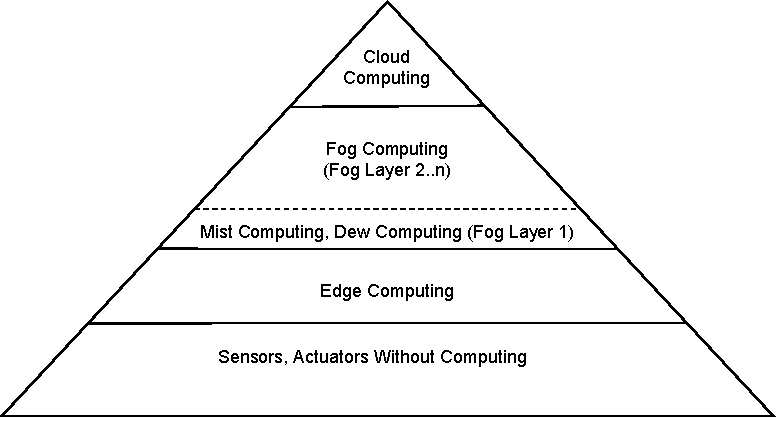
\includegraphics{Computing_Pyramid.pdf}
  \caption{The representation as a pyramid shows the increase in devices
  from the cloud to the edge (based on~\cite{DemystifyingFog}).}
  \label{Computing_Pyramid}
\end{figure}

\subsection{New Challenges}
At this point it should be said that the new computing paradigms
not only bring advantages, but also challenges for the developers
of IoT applications. In general, distributed systems are more complex
to implement than centralized systems. 
The distribution of the application components to the various
nodes between cloud, fog and edge increases the implementation
effort enormously. Due to the increasing heterogeneity of software
and hardware, a high level of platform independence is required
for the application.
In order to minimize the implementation effort, developers can now
choose from a large number of reference architectures~\cite{ComparisonIoTPlatformArchitectures}.
In the commercial sector, there are ready-made IoT platforms
(e.g. Microsoft Azure IoT, Amazon Web Service IoT, IBM Watson IoT)
for immediate use.

Other challenges are ensuring privacy and a possible dependency on providers.
These two aspects are already problematic for applications in cloud computing.
Further decentralization through fog and edge computing exacerbates
both problems. As in the cloud, fog nodes can also be public and offered
by external service providers. For example, a city administration could
provide several public servers as fog nodes to support smart city applications.
Despite the increase in providers, IoT application developers must watch
out for a vendor lock-in~\cite{VendorLockIn} and encapsulate their software components
against provider-specific \emph{application programming interfaces} (APIs).

When using edge and fog computing, external nodes can be included
in the routing process. In this case, the question arises why
the owners of the (resource constrained) nodes would allow data
to be forwarded. One possible solution for this
is incentive-based routing~\cite{RoutingIssuesSurvey}.


\section{Routing Algorithms}
The aim of routing is to find optimal paths for network traffic.
Typically this is the least expensive path. Various metrics
(e.g. delay, traffic jam situation, energy consumption, etc.)
are conceivable when determining the costs. Computer networks
are modeled as a graph in order to describe routing algorithms
based on them. Routing algorithms form the foundation for
routing protocols. In the TCP / IP stack, routing
protocols are assigned to the internet layer above IP~\cite{Tanenbaum}.

Routing algorithms use the optimality principle
to find optimal paths. Tanenbaum and Wetherall~\cite{Tanenbaum} describes the
principle as follows: \emph{``if router $J$ is on the optimal path from router $I$ to router $K$, then the optimal path from $J$ to $K$ also falls along the same route.''}. According to this principle,
the optimal paths from one node to all other
nodes form a tree, which is referred to as a sink tree.
Figure~\ref{sinkTree} shows an example of a sink tree (b), which
was obtained from graph (a). Routing algorithms
construct and manage sink trees for all nodes in a network.~\cite{Tanenbaum}
\begin{figure}[htpb]
  \centering
  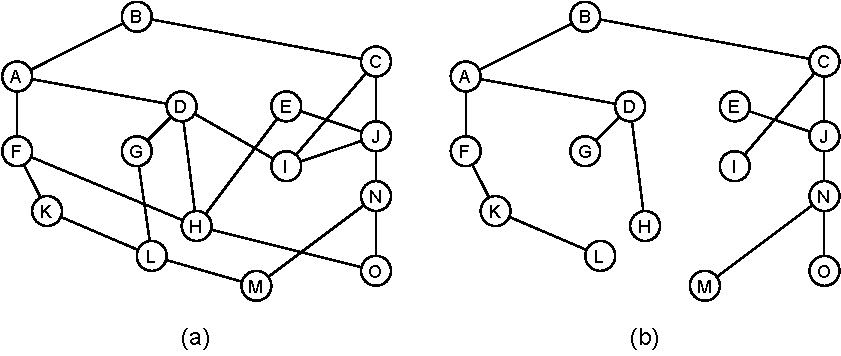
\includegraphics{sinkTree.pdf}
  \caption{(a) A network is modeled as a graph. (b) A sink tree with node B as the root.~\cite{Tanenbaum}}
  \label{sinkTree}
\end{figure}

\subsection{Routing Algorithm Classification}
Routing algorithms can be classified in a variety of ways.
Figure~\ref{figure_routing_classification} lists the classifications frequently
mentioned in the literature.
A first classification can be made according
to the place of execution. A centralized variant is possible
if the networks are not too widely distributed.
In this case, a selected, high-performance node can serve
as the network control center. This node has knowledge
of the entire network and can therefore calculate optimal
routes. All other nodes ask the control center whenever
they want to know an optimal route for forwarding data
to a destination node. Centralized routing procedures have
the same difficulties as centralized components
in distributed systems (scaling, security,
fault tolerance, performance bottlenecks).
Because computer networks naturally have a highly
distributed character, a distributed execution
of the routing algorithms on the nodes is traditionally
used~\cite{Kurose}. \emph{Software Defined Networking} (SDN) offers a new variant,
in which the routing in the control plane is carried
out in a logically centralized manner~\cite{Kurose}.
However, the routing algorithm still runs physically on each node~\cite{Kurose}.
The classification into static or dynamic (also called adaptive)
relate to the degree of change in the network topology~\cite{Tanenbaum}.
Static routing algorithms are preferable if the topology
rarely changes and the routing choice is clear~\cite{Tanenbaum}.
In this case, the routing algorithm is initially
executed once and the calculated routes are ideally used until
the end of the network's service life.
In the event of changes, the network administrator
can intervene manually or the routing algorithm is
completely restarted. However, in practical use are often dynamic algorithms.
These change their routes
depending on the topology or network traffic. Dynamic
algorithms are more complex because the nodes have to
keep their routing information up to date at all times.
For this purpose, the nodes can operate either
in direct response to changes (reactive) or
periodically (proactive)~\cite{Schiller}.
Proactive protocols have a higher update rate than
reactive protocols. Proactive protocol-type nodes flood
the network regularly to keep their routing information
up to date, even when there might be no traffic~\cite{Schiller}.
Reactive protocols try to avoid this problem by only
establishing a communication path between nodes when
it is actually needed~\cite{Schiller}.
\begin{figure}[htpb]
  \centering
  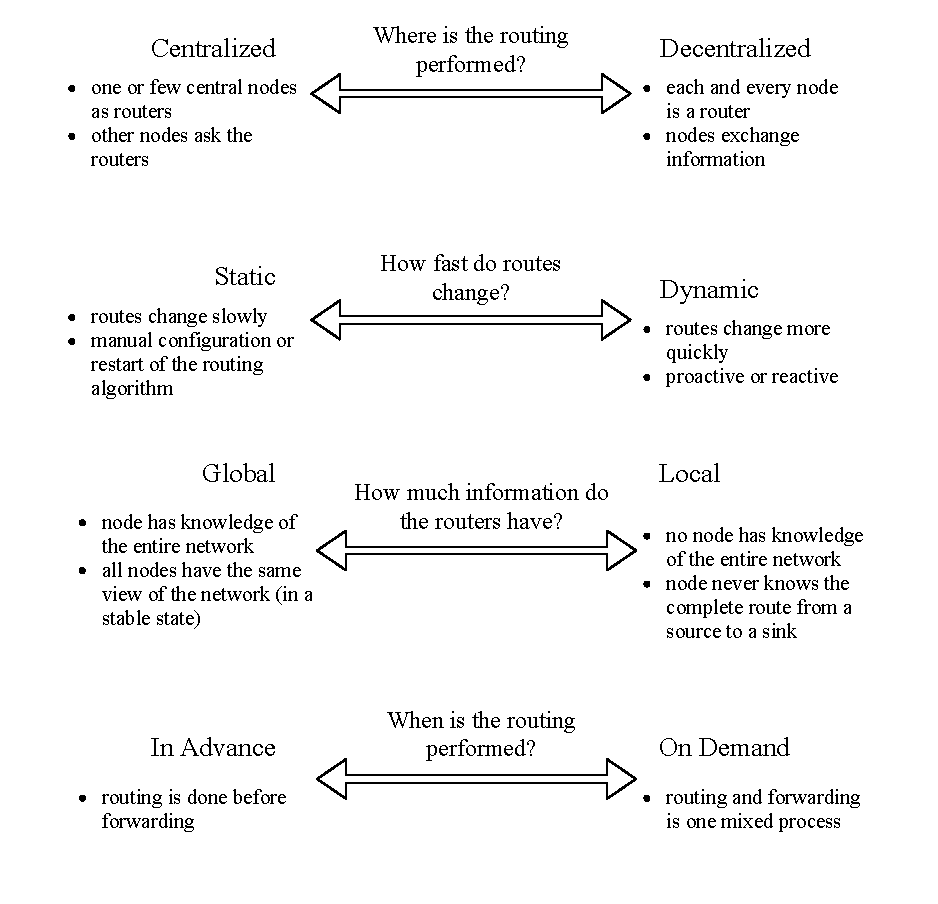
\includegraphics[scale=0.9]{figure_routing_classification.pdf}
  \caption{Overview of a possible classification of routing algorithms.}
  \label{figure_routing_classification}
\end{figure}

Another classification can be made with the question
of how much information a node has about the topology~\cite{Kurose}.
The routing table is an essential part of this information.
Typically, each node maintains such a table.
The table contains an entry for every other node in the network
with information about that node.
This includes the preferred communication line to this node as well
as estimates of distance (e.g. number of hops), time or costs.
The way in which routing tables are constructed differs
between nodes with only locally available information and nodes
with global information. The routing algorithm, in which the nodes
only use local information, is called distance vector routing
or distributed Bellman-Ford routing algorithm~\cite{Tanenbaum}.
With this algorithm, every node saves the distance to every
other node (distance vector).
In the first step, a node determines the distance
to its directly accessible neighbors by exchanging messages.
Then the node sends its distance vector to all neighbors
and it also gets a distance vector from each neighbor.
In this way, the node can already determine the shortest
route to the neighbors of the neighbors.
Each node updates its distance vector when it changes
and sends it back to all neighbors. After a finite number
of iterations, each node then arrives at its final
distance vector~\cite{Tanenbaum}. In the final version, this contains
the summed up distance of the shortest route to
every other node as well as the next hop for
this route. With the distance vector, any other
metric (hop count, delay, etc.) can actually
be used instead of the distance. It is only important
that the sum of the individual numbers
makes semantic sense.

The algorithm with global information at each node
is called link state routing. The first step
in the link state algorithm is similar to
the distance vector algorithm. All nodes first exchange
information with their neighbors in order to
discover the link costs and accessibility~\cite{Tanenbaum}.
Then each node builds a packet with its initially
learned knowledge and sends it to every other
node in the network~\cite{Tanenbaum}. Because the nodes do not
know each other at first, the network is flooded
by each node. Flooding describes the technique
in which the recipient forwards incoming packets
to all outgoing links except the sender's~\cite{Tanenbaum}.
This reveals the entire topology to each node.
In the next step, the shortest paths to all other
nodes are calculated locally using
the Dijkstra algorithm~\cite{Tanenbaum}.

Routing algorithms can be classified according
to the point in time when the algorithm is executed.
One possibility is to handle the routing process
in advance. In a first phase, the algorithm is executed
in order to construct the routing tables for the nodes.
Then, in a second phase, the data can be forwarded
on the basis of these tables. In dynamic networks,
the tables are maintained in the event of changes
in the topology or at regular intervals
(e.g. every 30 seconds~\cite{Schiller}).
On the other hand, in highly dynamic networks
(mobile ad-hoc networks), the route may already be
out of date when the first attempt at forwarding is made.
Assuming that there is light network traffic,
it may be appropriate in this case to mix the
routing process with the forwarding~\cite{Schiller}.
This form of routing is called on demand routing.
With on demand routing, the sender floods the network
every time to find the recipient in the current situation.

\subsection{Routing in Internet of Things}
In the literature~\cite{RoutingIssuesSurvey}\cite{routingSurvey}, routing in the IoT is often associated
with routing in \emph{Low-Power and Lossy Networks} (LLN). Constrained networks like LLNs are the dominant network type
at the edge and sensor layer. There are unconstrained networks at the fog and cloud layer.
In the case of unconstrained networks, proven routing protocols such as OSPF or IS-IS,
which have been used on the Internet for decades, can be used~\cite{Tanenbaum}.
Routing protocols for LLNs, on the other hand,
emerged with the development of IoT and are therefore comparatively new.
Compared to traditional networks, LLNs naturally have different
routing requirements. They are typically wireless, meshed, multi-hop, and lossy.
The nodes are constrained nodes that may work under severe resource constraints~\cite{rfc7228}.
Accordingly, the aim is always to reduce the traffic and the load on the nodes
to a minimum. In order to meet the requirements, two strategies have emerged:
\begin{enumerate}
 \item The routing table per node is kept as small as possible and only calculated locally.
 Some protocols completely dispense with routing tables and rely on on-demand routing or source routing
 (the route is already included in the data package). The distance vector algorithm forms the basis
 for many protocols for route calculations. Link state algorithms, however, are not used as the basis.
 \item Routing decisions are left to the more powerful nodes at the edge of the network
 as far as possible. These nodes are mostly gateways with an Internet connection.
 The routing table for these nodes can be more extensive than the tables within the network.
 For example, in a WSN, there are one or a few data sinks. These data sinks are mostly
 nodes that are more powerful than the sensor nodes and can therefore take on more routing tasks.
\end{enumerate}

\subsection{Routing Protocol for Low-Power and Lossy Networks}
After a detailed analysis of existing routing protocols with regard
to the requirements for LLNs, a working group of the
\emph{Internet Engineering Task Force} (IETF) developed the
\emph{Routing Protocol for Low-Power and Lossy Networks} (RPL)~\cite{RPLApplications}.
RPL has been standardized in RFC~\cite{rfc6550} since 2012 and is considered
the de facto routing standard in LLNs~\cite{RPLApplications}.
In the meantime there are various extensions (e.g. optimization
of energy consumption, consideration of the geographical
location and much more) for application-specific variants~\cite{RPLApplications}.
RPL works decentralized, proactive, local and in advance.
On-demand discovery to specific destinations is also supported~\cite{rfc6550}.

The basis for the routing is the \emph{Destination-Oriented Directed Acyclic Graph} (DODAG).
A DODAG is like a sink tree in which not only the optimal routes,
but also alternative routes are permitted. The alternative
routes are to protect against failures or changes in the topology
and are only active when required. The DODAG root is usually
a more powerful node that acts as a gateway. If several such
nodes exist, then several DODAGs can also exist in parallel.
The DODAG is destination-oriented because all nodes are oriented
towards the root node as the destination. Depending on the root,
each node calculates its rank in the DODAG. With the help
of the rank, the graph can be kept acyclic. A rank is a numerical value,
which reflects the position
of the node in relation to the root. The root always has the lowest rank.
Starting from the root, the rank rises strictly monotonic
to the leaves. That is, the direct descendant nodes of the root
have a greater rank than the root, but a lower rank than their
own descendants. When constructing the DODAG, a node ignores
certain messages from nodes with a greater rank and a
hierarchy can thus arise that is acyclic.

Three control messages are used for the construction and maintenance
of the DODAG, which are sent via the
\emph{Internet Control Message Protocol version 6} (ICMPv6).
These messages are called \emph{DODAG Information Object} (DIO),
\emph{DODAG Destination Advertisement Object} (DAO)
and \emph{DODAG Information Solicitation} (DIS).~\cite{RPLWhitepaper}
\subsection{Construction}
The construction always starts at the root node with
a broadcast of DIOs. The DIO message contains
information about the DODAG as well as the rank
of the sender. A node within radio range and the
corresponding protocol stack receives and understands
the message. The message contains information
about the DODAG as well as the rank of the sender.
The recipients can now decide how to proceed based
on this information and their own condition.
Assuming a recipient $B$ is still unknown to the DODAG
and therefore decides to join:
\begin{enumerate}
 \item $B$ first calculates its own rank based on the rank of the sender.
 \item $B$ inserts the sender into its set of parent nodes.
 \item $B$ saves the sender as a preferred parent node. 
 A preferred parent node is the next hop for all data transmissions in the direction of the root.
 \item $B$ builds a new DIO message that now contains its own rank.
 \item $B$ broadcasts the DIO message and now becomes a sender itself.
\end{enumerate}
The rank is calculated with a so-called \emph{Objective Function} (OF).
The OF is an application-specific function that combines the rank of a predecessor
and usually other metrics such as link costs or the state of the own node
(e.g. energy) in a mathematical formula in order to calculate a new rank~\cite{rfc6552}.
The external information for the rank calculation is contained in a DIS message
from the predecessor. Accordingly, the rank of a node $N$ is equal to $N = OF(DIS)$.
Assume that recipient $B$ is already included in the DODAG.
Then $B$ has already calculated its rank at least once.
$B$'s current rank is now compared to the potential rank $X$,
where $X$ is calculated by $X = OF(DIS)$.
If $B$'s rank is less than $X$, the DIS message is not processed, but rather discarded.
If $B$'s rank equals $X$, $B$ can add the sender to the set of parents.
Whether $B$ actually includes the sender in the set of parents
and perhaps also identifies the sender as the preferred
parent node depends on the implementation~\cite{rfc6550}.
If $B$'s rank is greater than $X$, $B$ sets its rank equal to $X$ and sets
the sender as the currently preferred parent node.
The set of parent nodes is reset and the sender is now the only member in this set.
In addition, $B$ broadcasts DIO messages to the other nodes.
Whenever a node changes its rank,
it is communicated to the other nodes with a DIO message.
The other nodes process the DIO in the same way as $B$
and construction of the DODAG continues. 
As soon as the leaves discard the last DIOs, the DODAG is ready.

The construction is explained using an example in Figure~\ref{DIO}.
A meshed network is shown in (a). Node $A$ is the root.
The dotted lines represent the available links.
A has three reachable neighbors $B$, $C$ and $D$, whose links
are indicated by abstract costs $3$, $1$ and $4$.
In (b) the DODAG construction is started.
The root sets its own rank to $0$\footnote{In this example the constant BASE\_RANK~\cite{rfc6550} is used.} and sends DIOs to its neighbors.
For the sake of simplicity, this model assumes that the latency is identical
for all messages. The sum of the abstract link costs is taken as the OF,
which results in the shortest paths to the root according to these costs.
As shown in (c), nodes $B$, $C$ and $D$ process the DIOs by calculating
the rank and then also performing a DIO broadcast.
The nodes have saved the root in their parent set and also
set it as the preferred parent node, as illustrated by
the solid arrow. In (d), after receiving the DIO from
node $C$, node $D$ changes its preferred parent node.
Because the rank of $D$ is greater than $OF(DIS)$,
where DIS is the message of $C$
(rank of $D$ is $4$ and $OF(DIS)$ is $3$).
The final DODAG is shown in (e). Node $D$ adds node $G$
to its parent set because $OF(G)$ equals
to the value of $D$’s rank. In (f) it is illustrated
how the data is sent from the leaves towards the root.
In addition, a link failure at node $D$ is shown
as an example, which leads to a change in the
link to the alternative parent node $G$.
\begin{figure}[htpb]
  \centering
  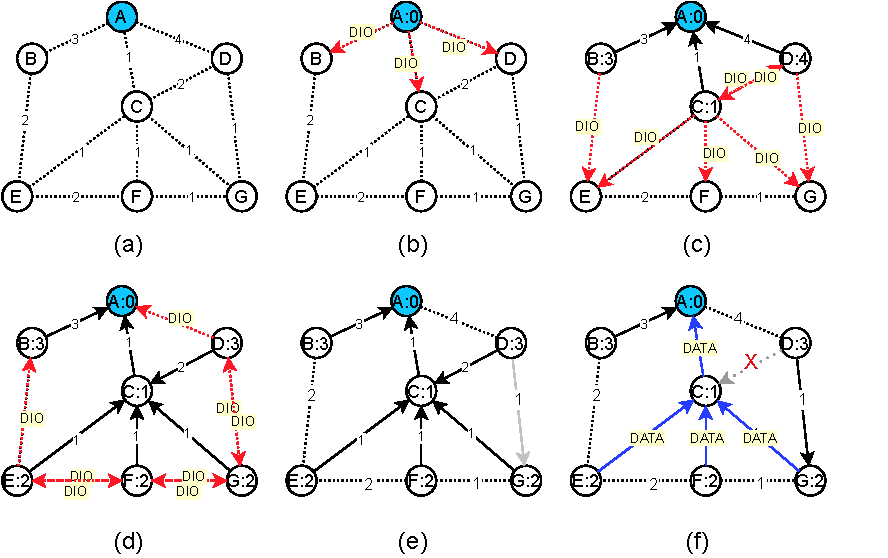
\includegraphics{DIO.pdf}
  \caption{Construction of a DODAG with multipoint-to-point traffic}
  \label{DIO}
\end{figure}
\subsection{Maintenance}
For the maintenance of the DODAG, RPL has been designed
as a proactive protocol. Each DODAG maintains a logical clock
called trickle timer. When the clock runs out,
a DIO broadcast is carried out in order to track down changes
in the DODAG. In fact, DIOs are only sent
when the trickle timer initiates this.
A node resets the trickle timer when it enters
a new DODAG or when there are changes in the parent
set, preferred parent nodes or rank~\cite{rfc6550}.
The trickle timer influences the sending rate
of the DIO broadcasts and therefore has
a considerable influence on the performance
of the network~\cite{RPLMultiparent}. The trickle timer adapts to the
stability of the DODAG over time, i.e.
the transmission rate decreases because the timer increases.
With the trickle timer, RPL uses a
compromise between topology changes and network load.

Nodes that are unknown to the DODAG can listen to DIOs and
then decide whether to join. If a node wants to speed up the joining process,
it can carry out a DIS broadcast.
DIS messages force the immediate sending of a DIO by resetting
the trickle timer at the recipient (if certain flags
in the message do not prevent it)~\cite{rfc6550}.
\subsection{Downward Routes with Routing Tables}
The construction with DIOs leads to so-called upward routes,
in which only multipoint-to-point traffic is possible.
So far, only the child nodes know their parent nodes.
DAO messages are used to enable downward routes as well.
DAOs are sent from a node to its parent nodes so that
the parents also know about this relationship.
This creates routing tables and enables point-to-point
or point-to-multipoint traffic.
The way in which the downward routing happens depends on the mode used.
The network operator can choose between the mode Storing
(fully stateful) or Non-Storing (fully source routed)~\cite{rfc6550}.
In the storing mode, each node, with the exception
of the leaves, stores a routing table for all reachable
destination nodes and the next hop. The next hops are
the child nodes. If a node has to forward a data packet
whose destination cannot be found in its table, then
it is sent to the preferred parents by default.
To construct the tables, DAOs are sent at least at the following times:
\begin{itemize}
 \item If a node selects another node as a parent node,
 then it sends the selected node a DAO message with its own reachable destinations.
 The number of destinations increases with the proximity to the root.
 A leaf node has no destinations, while the root can reach all nodes in the DODAG.
 Using this DAO message, the recipient can add the sender as the next hop and the destinations
 that can be reached via this hop in the routing table.
 \item If a node changes a parent node, then it sends the old parent
 node a special DAO, which is called No-Path~\cite{rfc6550}. This allows the
 receiver to remove the sender and the destinations that can be
 reached via this node from its routing table.
 \item If a node has processed a DAO, then it sends a DAO to all of its parent
 nodes so that they also update the routing tables~\cite{rfc6550}. The further
 sending of DAO messages ends as soon as the root is reached.
\end{itemize}
To reduce the number of messages, recipients of a DAO should not immediately
send another DAO to a parent node. Instead, an implementation-dependent
timer called DelayDAO is awaited first in order to aggregate DAO
information from other nodes. The timer starts as soon as the first
DAO has been received. Further DAOs do not reset the timer.
When the timer expires, the node sends its DAO.~\cite{rfc6550}

Figure~\ref{StoringMode} shows an example of the appearance of routing
tables in a simple DODAG. The root can target all nodes as destinations,
while leaves have no destinations and therefore no routing tables.
Point-to-point traffic always travels from the sender in the direction
of the root to the next common ancestor and then from the
ancestor down to the destination. For example, node $X$ intends to send
data to node $V$. $V$ does not appear as a destination in $X$'s routing
table ($X$ has no table anyway). Then $X$ sends the data towards
the root. In this example, the preferred parent node $Y$ is also
the closest common ancestor of $X$ and $V$. $Y$ forwards the data
to $W$, who in turn forwards them to $V$.
\begin{figure}[htpb]
  \centering
  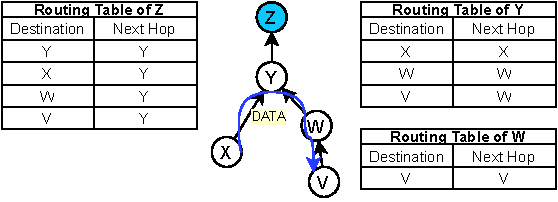
\includegraphics{StoringMode.pdf}
  \caption{Routing tables and point-to-point traffic in storing mode (based on~\cite{RPLHybridMode}).}
  \label{StoringMode}
\end{figure}

In the non-storing mode, only the root has a routing table.
DAOs are only sent to the root via unicast. Accordingly,
DAOs travel unprocessed via the preferred parent links
of the intermediate nodes to the root. With its routing table,
the root can define complete paths to destinations.
When sending data packets to a destination, the complete path
is included in a source routing header~\cite{RPLHybridMode}.
Figure~\ref{NonStoringMode} shows an example of the point-to-point traffic flow.
Suppose node $X$ intends to send data to node $V$.
In the non-storing mode, only the root node takes
on the routing task. $X$ sends the data via its preferred
parent node to $Y$, which in turn simply forwards
the data to the root. The root $Z$ knows all paths
to all destinations. $Z$ inserts a source routing
header into the data packets, which 
contains the path $Y$, $W$, $V$.
\begin{figure}[htpb]
  \centering
  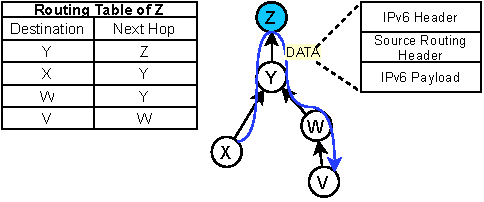
\includegraphics{NonStoringMode.pdf}
  \caption{Routing tables and point-to-point traffic in non-storing mode (based on~\cite{RPLHybridMode}).}
  \label{NonStoringMode}
\end{figure}

\section{Database Systems}
The billions of tiny devices in the IoT produce enormous amounts of data that have to be managed. Initially, the data was managed in the cloud. However, with the new computing paradigms, the processing of the data is shifted towards the edge nodes. Consequently, data should also be stored on the edge nodes or at least on nearby fog nodes. Database systems are the means of choice for persistent storage and efficient retrieval of data. They are available for a variety of data models (e.g. relational, XML, key-value) and platforms (e.g. parallel servers, main memory, cloud)~\cite{HM3P}.

\subsection{Query Processing}
 For each data model there is a language to query the data. The query language is the interface to the application. With one language as the interface, the database system remains both application-independent and flexible. Database query languages are declarative so that, as a practical matter, applications only need to describe what the result of the query should be. The database system must translate the declarative query into an internal query that shows how the result is to be calculated. However, there can be several possible solutions for calculating the result for a declarative query. The choice of one good solution is made after several optimization steps. Overall, query processing goes through multiple phases that are similar in all typical database systems~\cite{SWBook}.

The phases are shown in Figure~\ref{queryProcessingPhases}. Processing starts with the parsing of the declarative query in an \emph{abstract syntax tree} (AST). The syntax of the query is checked against the grammar of the query language. In the next step, any syntactic sugar that may be present is removed in order to simplify further processing\footnote{This phase is often omitted especially for simple query languages.}~\cite{SWBook}. After these preparatory steps the AST is transformed into an operator graph.
An operator graph consists of nodes with logical operators and nodes that represent data sets. Logical operators still have a declarative character. The initial logical operator graph serves as input for the logical optimization. With the help of equivalence rules, the operator graph is restructured in such a way that the execution time (or costs) are as small as possible without changing the output~\cite{SWBook}. The choice of rules is based on heuristics and cost estimates~\cite{Kemper}.
Then the logical operator graph is translated into the physical operator graph. Here, the boundary between the logical and the physical level is exceeded~\cite{Kemper}. Each logical operator is replaced by a physical operator that specifies a concrete algorithm for implementation. Several physical operators can be selected for a logical operator. The choice is based on a cost model in which the physical properties of the storage (e.g. indices) are also taken into account~\cite{Kemper}. The physical operator graph is called the execution plan~\cite{SWBook}. Its execution finally leads to the query result.
\begin{figure}[htpb]
  \centering
  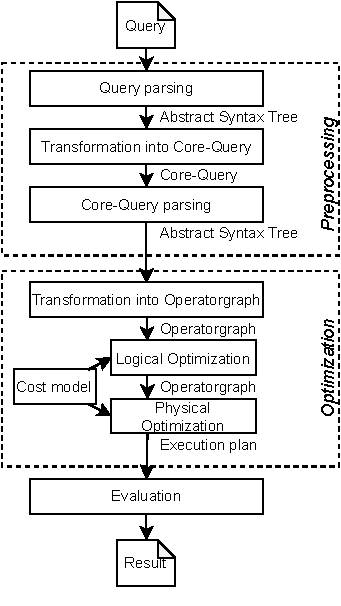
\includegraphics{queryProcessingPhases.pdf}
  \caption{Example of the query processing phases (based on~\cite{SWBook}).}
  \label{queryProcessingPhases}
\end{figure}

\subsection{Distributed Query Processing}
A distributed DBMS consists of autonomously working nodes, with each node having a DMBS instance and one or more databases~\cite{Kemper}. The nodes are located geographically apart and are connected to one another via a communication network in order to work together on database operations~\cite{Kemper}. The processing of queries for data from several nodes is one such operation that requires collaboration. The processing steps from Figure~\ref{queryProcessingPhases} are no longer carried out entirely on one node.
Instead, the optimization part is separated into global optimization and local optimization~\cite{Rahm}.

The global optimization is carried out once for the DBMS instance that receives the query (also called the coordinator). When restructuring the operator graph, the properties of the data distribution are taken into account. The cost model is expanded to include communication costs (message size, number of messages) in particular. The coordinator also determines, among other things, the place of execution of the operators. The globally optimized operator graph is broken down into parts and the parts are sent to the appropriate nodes for further local processing. The DBMS instances of the nodes then carry out further optimization steps, taking into account their locally available cost model and the system status.
The proportion of the logical optimization within the local optimization or the proportion of the physical optimization within the global optimization depends on the locally available information. For example, the coordinator can already make physical optimizations if index structures are known.~\cite{Rahm}

\subsection{The Internet of Things Platform}
The platform of a DBMS is the execution environment for which the DBMS is built. There are many platforms on which DBMSs can run and depending on the platform, the system has to adapt to the peculiarities of the environment~\cite{HM3P}. The IoT platform is a relatively new field of research, which has gained momentum in the course of the paradigm shift from cloud processing to edge processing. DBMSs, which are adapted to the IoT platform, operate on cloud, fog or edge level, are often designed as stream DBMSs and are typically distributed or even \emph{peer-to-peer} (P2P).

IoT DBMSs are often geared towards stream processing because sensor networks usually generate data over a long period of time. One possibility is to extend the declarative query language to include commands for long-running queries. The processing is similar to that of the one time queries with a data flow through an operator graph. One difference is that the data flow runs continuously. In addition to continuous processing, batch processing can also be used. In the case of batch processing, incoming data are grouped within a certain time window in order to process them together when the time has elapsed. Some systems also offer event-based processing. For example, additional rules can be defined in the query that generate new data when a certain event occurs.~\cite{StreamDBSSurvey}

Basically there are different degrees of distribution for databases in the network~\cite{DistributedDBS}. Depending on the fog and edge level as well as the requirements of the IoT application, DBMSs are in the continuum between centralized and highly distributed systems. For example, in a warehouse approach~\cite{WSNDatabases}, a first level fog node (mist node) could have a central DBMS with a database and thus be the point of contact for WSNs. If, for example, the data on the fog level is to be distributed across multiple databases from multiple fog nodes, then a distributed DBMS can be used.

For IoT applications with a relatively small number of database nodes and little or no changes in the number, a distributed DBMS can be sufficient. The alternative for upscaling systems is the P2P approach~\cite{DistributedDBS}. In a pure P2P system, each node has the same functionality, so that the functionality scales with the number of nodes. With regard to database systems, each node has a DBMS, so data storage scales with the number of nodes. For efficient data dissemination and search, structured P2P systems based on \emph{distributed hash tables} (DHT) are preferable if the costs of overlay routing can be borne~\cite{TinyTurrent}.

\subsection{Wireless Sensor Network Database Management Systems}
With the increasing number of sensors in a WSN, the collection and evaluation of the data becomes more difficult~\cite{WSNDatabases}. Researchers have been dealing with this problem for two decades. One approach is to view the entire WSN as one database~\cite{SNasDB}. This is made possible by a WSN DBMS whose instances run on the sensor nodes and abstract these sensors using a database query language. Controlled by a query language, the DBMS instances carry out operations such as aggregation and filtering, thereby reducing network traffic and consequently also energy consumption in the WSN. According to today's understanding, this approach falls into the category of edge computing.
A WSN DBMS is a distributed system that abstracts from the WSN. A query language is provided as an interface for abstraction for an application. Three features are characteristic of a WSN DBMS:
\begin{enumerate}
 \item There is an extension of the query language for controlling the sensors. It takes into account the fact that smart sensors have control over when and how often environmental measurements should take place~\cite{TinyDB}. Long-term queries are also possible, as sensors can typically take measurements over a long period of time~\cite{Cougar}.
 \item The processing of the query is mixed with the routing algorithm~\cite{SNasDB} and therefore takes place within the internet layer in the TCP/IP model. Sensor nodes do not need higher protocols for communication and work more resource-efficient. This type of query processing is also called in-network query processing~\cite{SNQP}.
 \item Due to the limited resources of the sensors, most of the features of conventional DBMS (e.g. transactions, flexible schemes) are not available or are only available in rudimentary form. Instead, the focus is on in-network query processing. In some literature, a WSN DBMS is therefore also simply referred to as \emph{Sensor Network Query Processor} (SNQP)~\cite{SNQP}.
\end{enumerate}

Examples of such systems are TinyDB, COUGAR, SINA or Corona, which are compared with one another in ~\cite{WSNDatabases}.

\section{Modeling and Simulation}
Modeling has a long tradition in research and development.
Models help to draw conclusions about reality by showing
a simplified representation of reality. Modeling can be
used when the real object is too complex to analyze directly.
A model is essentially characterized by its simplification.
This means that a model is an abstract object of the real object
in which only a few aspects that are relevant for the modeler
are considered. According to Weisberg~\cite{Weisberg}, 
a total of three categories of models can be distinguished:
concrete, mathematical and computational. 
The latter models are increasingly used in science~\cite{Weisberg}.
This models are described algorithmically to be carried out on computers.
The execution is called a simulation and the program
that creates the simulation can be called a simulator.

The computational model is related to its original system.
This relationship is necessary in order to be able to draw
conclusions about the original system.
The relationship is shown by properties that the model
and the original share, which are 
still shared even after operations~\cite{Weisberg}.
Figure~\ref{figure_model} illustrates the relationship between a model and its original.
For example, a model of an IoT device may be similar
to the real device in that it behaves the same way
under modeled operations as the real device 
behaves or would behave under real operations.
\begin{figure}[htpb]
  \centering
  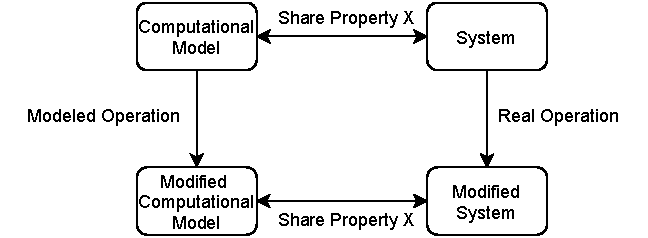
\includegraphics{figure_model.pdf}
  \caption{Relationship between a computational model and its system (based on~\cite{SpezModScript}).}
  \label{figure_model}
\end{figure}

\subsection{General Benefits}
If a complex problem is to be solved,
then a useful approach is the following:
First, strong assumptions are made about the object
of investigation, within which the problem can be
solved more easily.
The assumptions are then gradually
weakened in order to approximate the real conditions, because an attempt to solve the problem directly and without strong assumptions can reduce the chances of success.
Modeling can be the backbone of this approach.
The problem to be investigated is represented as
a model and first solved in the modeled world in order
to then solve it in reality by refining the model or by
eliminating the model.


\subsection{Benefits for Software Engineering}
In computer science, and especially in software engineering,
modeling and simulation can be used in the development
and analysis of large, complex systems.
Models can be used at many points in the software development
process. Examples of good times are the integration test and the system test.

In the integration test, the interaction of the components
of the system is tested. Because not all components are available
for integration at the beginning of development, a strategy
is required that defines the sequence in which the 
components are implemented. Dependencies on components
that do not yet exist can initially be resolved
using stubs. For a deeper analysis of the correct
integration, a model can be used as a stub.~\cite{BasisTest}

During the system test, the system is tested as a whole.
The runtime environment should come as close
as possible to the later productive environment.
If it is too complex or not possible to use
the production environment, modeling
this environment can help.~\cite{BasisTest} The simulator can be designed
as a framework for seamless integration of the system
into the modeled environment. The program start point
is then with the simulator and no longer with the system.

\subsection{Benefits for Engineering of Distributed Systems}
In the past few decades, many simulation 
frameworks have been built to study the 
behavior of large-scale distributed systems~\cite{BigDataSim} like
cloud, grid, IoT or P2P systems. From a certain degree
of scaling, their behavior can be tested more easily
in a simulated scenario.

This is because the necessary infrastructure,
which includes a large number of different physical
devices, is typically not made available to third
parties by any commercial provider~\cite{SimOverview}. Constructing
your own physical infrastructure is too costly
and too resource and time consuming~\cite{SimOverview}. A simulation
framework can solve this problem. In addition,
different scenarios with different hardware and
network resources can easily be tried out
repeatedly with a simulation~\cite{BigDataSim}. Thanks to the
repeatability, regression tests~\cite{BasisTest} are now also
possible, which can accelerate the development
of software components. In addition, due to its
repeatability, the configuration data of the
simulation can be shared with other developers in
order to obtain better validation of the results~\cite{BigDataSim}.

Another important aspect when developing
IoT applications is the ideal distribution
of the components within the infrastructure.
IoT environments pose a particular challenge
here with their large number of heterogeneous
devices of different performance levels and
distribution across cloud, fog and edge.
Figure~\ref{figure_deployment} illustrates the software component deployment problem that can occur in IoT system design~\cite{AnalyzeQualities}.
\begin{figure}[htpb]
  \centering
  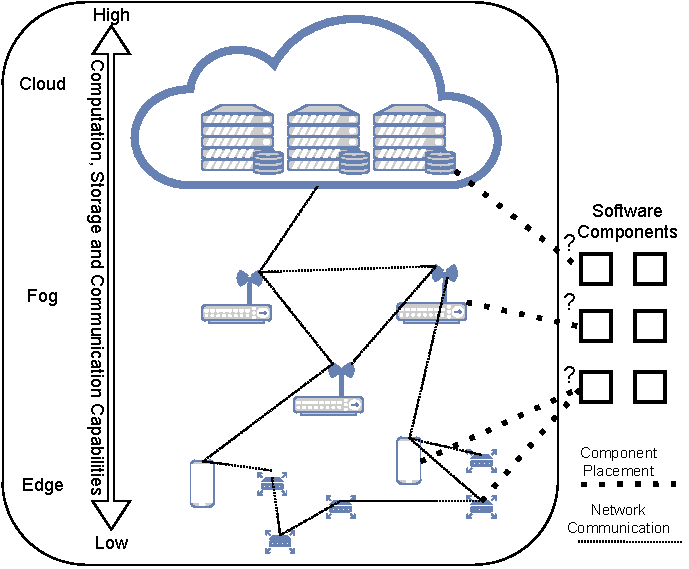
\includegraphics{figure_deployment.pdf}
  \caption{Illustration for the software component deployment problem~\cite{AnalyzeQualities}.}
  \label{figure_deployment}
\end{figure}

\subsection{General Challenges}
The modeler faces the difficulty of determining the required
level of accuracy of the abstraction.
For this purpose it can be useful to divide the system into its components and then to identify the respective features individually.
Some components are obvious and as such
are easy to determine. Other components
are not immediately apparent because
they may not occur in the real, actual system,
but rather represent external influences
on the system.~\cite{SimJavaTutorial}

Once the components have been determined, the modeler
must now determine the accuracy of the abstraction
for each component. Here one encounters
the following dilemma:
If the model is kept too general,
then it weakens the advantages of the modeling.
If the model gets too specific,
then the simulation can be too slow and
the model can also be wrong.
Because the finer and more complex the model, the more likely it is that the assumptions made contain errors.
It is helpful not to lose focus on the actual
purpose of the simulation.
A model is usually developed for a certain
set of goals, and if a model is valid for
one goal, it doesn't have to be
valid for another either~\cite{BuildValidModels}.

\subsection{Discrete Simulation}
Software systems are discrete systems. Their execution can be modeled as a sequence of countably many states. Therefore, a discrete simulation can be used for these models.
In a discrete simulation, there is a global, logical clock that advances in discrete steps. In the case of a logical clock, the physical time is not of interest. Instead, the order of events is of interest, i.e. whether an event occurs before or after another event. If an event occurs before another event, then the logical clock of the first event is smaller. In this way the correct order of events can be determined. In general, there are two types of discrete simulation. In the \emph{discrete time simulation} (DTS), the progress of the clock determines the chronological order of the events. DTS is a time-driven approach~\cite{DissSimulation}. In the case of \emph{discrete event simulation} (DES), on the other hand, the events determine the progress of the logical clock. DES is an event-driven approach~\cite{DissSimulation}.

\subsection{Discrete Time Simulation}
DTS is easier to understand than DES, but there
are pitfalls in terms of accuracy~\cite{SimAccuracy}.
The simulation is based on a division into
fixed time intervals within which a set
of objects can perform modeled operations.
The objects are also called entities.
They form the building blocks of the system to be simulated.
The global clock is incremented according to the
fixed intervals. After each increment, all entities are scanned
and changes are made to the states according to
the previous time interval. Assuming a fixed time increment is $\Delta$,
the DTS can be explained as follows:
\begin{enumerate}
 \item Increment clock $C$ to $C + \Delta$.
 \item Search all entities for events that would 
 have happened in the time interval from $C$ to $C + \Delta$.
 \item Execute these events and update the states of the entities.
 \item As long as an end condition is not fulfilled, start again at step 1.
\end{enumerate}

An inaccuracy of the time-based method is
that the entities can only change their states
at the same time within a time step, although the state
changes do not occur at the same
time in reality~\cite{SimAccuracy}.
Another inaccuracy occurs due to the size-fixed intervals.
Choosing smaller time
intervals could increase the accuracy
of the simulation, but the performance
of the simulation execution is reduced~\cite{SimOverview}.
In addition, this method is less worthwhile if there
are many larger time steps. Each step
is processed regardless of whether there are really changes to the entities.
Buss and Al~Rowaei~\cite{SimAccuracy} come to the conclusion
in their comparative study that whenever
the choice between DES and DTS is possible,
the former should be chosen. DES is therefore also used in this master's thesis.

\subsection{Discrete Event Simulation}
With DES, the times at which the events occur determine the progression of the clock, which is why this method is also referred to as event-based or event-driven. At its core, a DES consists of entities, events and a scheduler. The scheduler manages the global clock and the order in which events occur. Every event has a defined point in time, which determines when the event comes into force. To maintain the correct order of occurrence, the scheduler keeps all future events in a priority queue.
The sorting criterion is the time of occurrence, so that removal from the queue always delivers the next event in time. In principle, DES is based on the processing of this queue of future events. Just like in DTS, events are tied to entities. Entities can perform modeled operations and communicate with other entities through events. In this way, events are messages between entities. DES can be roughly described by the following steps:
\begin{enumerate}
\item Start an initialization phase in which the first events are placed in the priority queue.
 \item Remove an event from the priority queue.
 \item If $x$ is the time of occurrence of the event, then overwrite the global clock $C$ with $C = x$.
 \item Process the event within the entity for which the event is intended. Processing can create new events that are placed in the priority queue.
 \item As long as the priority queue is not empty, start again at step 2.
\end{enumerate}

When creating new events during the simulation (step 4), the current global clock is added to the time of occurrence. If the time of occurrence is set to $x = 0$, then the event is part of the present and is still processed within the current clock tick. If the time of occurrence is $x > 0$, then it is an event that will only be processed in the future. $x < 0$ is not allowed. Because that would mean that the new events are in the past and the global clock will therefore go backwards in the next iteration.
\begin{figure}[htpb]
  \centering
  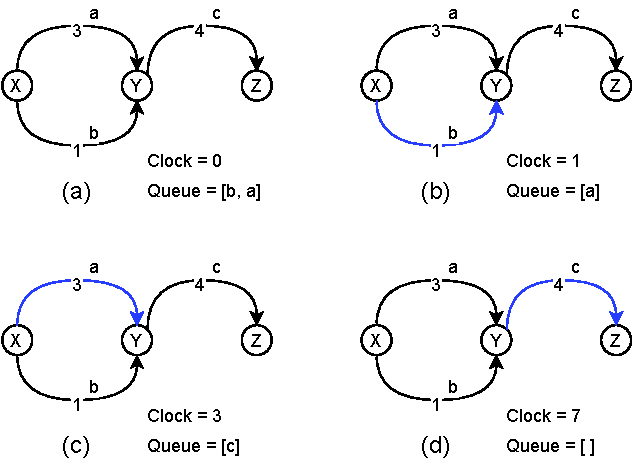
\includegraphics{figure_des.pdf}
  \caption{An example of the event-driven simulation process.}
  \label{figure_des}
\end{figure}

Figure~\ref{figure_des} illustrates an example of a simulation process. The system is modeled by the three entities $X$, $Y$ and $Z$. The order of execution of the modeled operations in the entities is determined by events $a$, $b$ and $c$. For this purpose, the time of occurrence as well as the sender and receiver must be specified for the events. Part (a) shows that in the initialization phase, entity $X$ generated two unconditional events $a$ and $b$, of which $Y$ is the receiver. Event $a$ is to be processed at $Y$ $3$ time units later after it has been generated, while event $b$ already reaches $Y$ after $1$ time unit. With the events, $X$ intends to trigger an operation in $Y$. The entity $Y$ does not yet generate any events in the initialization phase, but it links the generation of $c$ to the receive of $a$.
This means that there is an operation in $Y$ which, upon receive of $a$, generates event $c$. The entity $Z$ does not generate any events in this example. At the beginning the global clock is still $0$. In part (b) the simulation starts with the removal of the event with the smallest occurrence time from the queue. This is event $b$. The clock is set to $1$ and $Y$ is called to process $b$. In part (c) event a is taken from the queue. The time is now $3$. $Y$ processes a and then generates a new event c, which is added to the queue. Event $c$ is to be processed by $Z$ $4$ time units after it was generated. Since the clock is currently at $3$, the time of occurrence of the event is $7$. In part (d) the last event c is processed and the simulation ends with the clock $= 7$.

\subsection{Transient and Steady State}
In order to achieve representative results,
a simulation run is usually divided into two phases.
The first phase is known as the warm-up or transient period.
From a point in time to be defined,
the second phase is reached, which is referred
to as the steady state. In this second phase
the system is in a state in which it works
with a certain regularity and can be regarded
as stable. The point in time from which this
phase is reached is also the point in time
from which the measurements for the
simulation result begin.~\cite{SimJavaThesis}

If the question is asked how the simulation
should be started, the reason for the division
into transition phase and stable phase becomes clear.
To get started with the simulation,
unconditional activities must take place at clock $= 0$.
This can lead to a distortion of the modeling,
since there are practically no unconditional
activities in the real world.
The actual long-term behavior of the system can only
be observed when the simulation has been running
for a while and activities build on one another.

In the case of DES,
the priority queue does not initially contain
any events. At the start of the simulation the
possibility must be given to let the entities
generate the first unconditional events. For this
purpose, each entity has a start function that
is called by the scheduler at clock $= 0$.
The steady state is reached at the earliest with
the first simulation round, in which the first
unconditional event is taken from the priority
queue. However, it can also be customized
at a later point in time.

\subsection{Visualization and Configuration}
A simulation always has a specific purpose. If the purpose is a comparison between different models or model properties, a measurement is needed. The measurements can be output during or at the end of the simulation runtime. A text form (e.g. log file, console) or a graphic representation in the \emph{graphical user interface} (GUI) can be selected to visualize the output.

Before starting the simulation, a configuration option for the models is usually made available. A configuration file (e.g. XML, \emph{JavaScript object notation} (JSON)) or a GUI can be used for this purpose.
When setting the parameters, automatically generated random numbers are often added. In reality there are seldom fixed parameter values and a more realistic scenario can be simulated with the help of a random number generator. A seed is used for repeatable simulation results.

\section{Related Work}
% In a German thesis write: \section{Verwandte Arbeiten}

% !!!!!!!!!!!!!!!!!!!!!!!!!!!!!!!!!!
% !!! Your action is needed here !!!
% !!!!!!!!!!!!!!!!!!!!!!!!!!!!!!!!!!
%
% Replace with a detailed account of what other people have already
% researched concerning your thesis's theme. Even when (indeed,
% especially when) there has been only little or even no research by
% other people, you should explain in detail that this is the case and
% why it is the case. 
There are a variety of simulators for analyzing edge computing scenarios. Each simulator serves a purpose and offers different features. Depending on the simulation goal, one of the available simulators can be used. If relevant features are missing, an extension or a new development can be considered. 

Our simulator for distributed query processing is primarily intended to enable the integration of existing applications such as DBMSs. We analyze existing simulators according to the following features:
\begin{itemize}
 \item It must be possible to send real data in the network in order to save them in a DBMS.
 \item Configuration of different computing performance levels must be possible in order to model all types of devices in the computing pyramid.
 \item Real computing is required on the nodes to perform operators from the operator graph of a query.
 \item IoT network protocols with different data rates should be configurable.
 \item At least one IoT-compliant routing protocol should be implemented. In addition, it will be necessary to change the routing behavior due to the in-network operator graph calculation.
 \item Multiplatform capability for connecting multiplatform DBMS is advantageous. Kotlin is a suitable programming language for this purpose.
 \item Energy consumption is a helpful but not necessary feature for initial evaluations of the simulation goal.
 \item The measurement of network communication is more important. The question to be answered is whether the network load can be reduced by the distributed query processing compared to the central query processing.
\end{itemize}
Analysis results of existing work with regard to these features is presented in Table~\ref{table_simulators} and described in more detail below:

\begin{description}
\item [ns-3]\cite{simulator_ns3} is an event based network simulation framework written in C++. The byte-precision implementation of the TCP/IP stack with different protocols for each layer can be emphasized. The existing models are so precise that they can almost be compared with real protocol implementations. Therefore the simulator can also be used as an emulator for real existing protocols. ns-3 is primarily aimed at general networks on the Internet, so there are few IoT protocol models. IoT routing protocols are missing, but can be added via the API. A connection with real systems per node is supported by file descriptors. Simulated nodes can communicate with real processes, in which byte-precise link layer frames are written into a file or read from a file. Although this method is very precise, it is also slow when there is a lot of data traffic. A byte-precise simulation is less suitable for a simulation with hundreds of database systems. In addition, NS-3 has no multiplatform support. Customizations can be written using C++ or Python.
\item [COOJA]\cite{simulator_cooja} is an event based simulation framework for Contiki written in Java. Contiki is an operating system for low power wireless sensor nodes. Models of these nodes, which are written in C, can be emulated by COOJA directly on Contiki using a virtual machine. In addition, COOJA offers a simulation of sensor nodes without Contiki in Java. Similar to ns-3, the byte-precise modeling option should be emphasized. COOJA is designed for the IoT. Edge computing with real data must first be programmed via the API. In addition, simulation with complex external systems such as DBMS in a virtual machine is disadvantageous.
\item [FogNetSim++]\cite{FogNetSim} is a toolkit for modeling and simulating fog computing scenarios. It is based on the event-based framework OMNet++~\cite{OMNeT}. Various IoT network protocols, an energy module and various task distribution algorithms for fog computing can be used immediately. Edge computing can also be modeled by configuring hardware properties such as processor clock rate or main memory. However, the disadvantage of FogNetSim is that only modeled tasks and data can be simulated. This is why it is not possible to connect real external systems. In addition, C++ is not a multiplatform language.
\item [CloudSim]\cite{simulator_CloudSim} is a framework written in Java that serves as the basis for many event-driven IoT simulators. CloudSim models clouds through a set of data centers, which contain hosts, which in turn can run a set of virtual machines (VM). CloudSim offers extension points via interfaces and inheritance, which is used by the IoT simulators. The IoT simulators expand the event-based core and use the existing features such as energy and computing performance modeling. Some simulators~\cite{simulator_PureEdgeSim}\cite{simulator_recap}\cite{simulator_SatEdgeSim} prefer CloudSim Plus~\cite{simulator_CloudSimPlus}, which is a fork that increasingly follows software engineering principles. CloudSim or CloudSim Plus cannot be used for this thesis because the modeling is aimed at non-real computing tasks. Computing tasks are given abstractly with a number of instructions. In addition, there is no real data in the network or the possibility of integrating real applications. In addition, the extension leads to unnatural inheritance hierarchies in the IoT simulators. Classes such as Datacenter, Host and VM represent models that do not occur in the natural IoT environment, but must still be used for modeling IoT.
\item [IoTSim-Edge]\cite{IoTSimEdge} is an event-based simulation framework based on CloudSim. All settings for a simulation can be made in a JSON configuration file. This includes network communication, performance level and computing tasks. These features are inherited from CloudSim. IoTSim-Edge extends the features to include other edge computing-relevant features such as battery consumption, network protocols or mobility. Nevertheless, the computing tasks and data are fictitious. External systems can therefore not be connected. In addition, the simulator is written in Java, which limits its execution to the JVM.
\item[EdgeCloudSim]\cite{simulator_EdgeCloudSim} is another simulator based on CloudSim for edge computing scenarios. It offers network communication, mobility and the simulation of task processing at edge nodes. An XML file is used for the configuration. Compared to IoTSim-Edge, however, the modeling of protocols and energy consumption are missing. In addition, EdgeCloudSim is not suitable for simulating query processing because it does not work with real data. Besides, the execution is limited to the JVM.
\item[IoTSim-Osmosis]\cite{simulator_osmosis} is a simulator that focuses on the application composition. An application is modeled as a graph of microservices that are distributed in the computing pyramid.
IoTSim-Osmotic can provide answers to the deployment problem in IoT system design. The simulator also offers the features of IoTSim-Edge. CloudSim was used as the basic framework for the implementation. Accordingly JVM is the only platform on which the simulator can be executed. Real data and a connection to external systems is not supported. As with the other CloudSim-based tools, task processing and computing performance are only modeled abstractly.
\item[iFogSim]\cite{simulator_iFogSim} is also a simulation framework based on CloudSim. The algorithm for the placement of application components should be emphasized. The modeler can choose between cloud-only placement and edge-ward placement, and thus find answers to the software component deployment problem. In addition, data streams and their processing can be simulated. iFogSim can also be used for modeling edge computing scenarios, because different computing performance levels can be configured individually at the nodes. The configuration is possible with a JSON file or GUI. iFogSim is written in Java. Real data and external systems cannot be used. In addition, network protocols and routing protocols are not part of the simulator.
\item[PureEdgeSim]\cite{simulator_PureEdgeSim} is an event-discrete simulation framework for evaluating the performance of edge, fog, and cloud computing scenarios. Performance can be measured in network delays, energy consumption and task success rate. PureEdgeSim is based on CloudSim Plus and thus inherits the features for network communication and computing performance configuration. The modeling of the computing task success rate and a selection of orchestration algorithms for tasks can be highlighted. But PureEdgeSim, like the other CloudSim-based simulators, is not suitable for DBMS query processing and is also not multiplatform capable.
\item[YAFS]\cite{simulator_YAFS} is a simulator for IoT scenarios in fog computing. Features to be emphasized are the dynamic assignment of application components, mobility of nodes and the modeling of node failures. Similar to the other fog computing simulators mentioned, processing at edge nodes can be achieved by configuring the performance level. The simulator is event-based, written in Python and offers JSON files for the configuration of the scenarios. YAFS does not use any real data for the simulation. This means that it is not possible to integrate external applications.
\item[MyiFogSim]\cite{simulator_MyiFogSim} is an extension of iFogSim to offer mobility of nodes as a feature. Mobility is implemented through dynamic VM migration between cloudlets. In CloudSim-based simulations, which also include iFogSim and thus MyiFogSim, a Cloudlet is a model for a self-contained miniature cloud. An application is orchestrated as a set of cloudlets, with each cloudlet running in a simulated VM. With MyiFogSim different migration strategies and migration policies can be evaluated. However, the features necessary for distributed query processing are not supported.
\item[FogBed]\cite{simulator_FogBed} is a framework that extends the Mininet~\cite{simulator_Mininet} emulator. The essential feature of FogBed is the integration of real applications with virtualization. Virtualization offers the advantage of simulating limited hardware resources. FogBed uses Docker for this, in which real applications run in containers. Docker containers are lighter than VMs because they don't virtualize the operating system. Cloud, fog or edge computing scenarios can be simulated by using Docker containers as virtual nodes. Virtual nodes differ in the type of resource model used. A cloud can be mimicked by a disproportionately large allocation of resources, while edge devices are allocated only very limited resources. Containers are a possible approach for integrating large systems such as DBMS. In this thesis, a method is first developed to simulate a large number of DBMS instances by integrating a single real instance. The next step is then to evaluate the combination of the method with containers. However, this is no longer feasible within the scope of this work and will remain part of future work. FogBed cannot serve as the basis for the simulator in this thesis either, because it does not offer multiplatform support. FogBed is written in Python. In addition, there is no support for network protocols or IoT routing protocols.
\end{description}
\newcommand{\RNum}[1]{\uppercase\expandafter{\romannumeral #1\relax}}

\begin{table}[htpb]
\resizebox{\textwidth}{!}{
    \begin{tabular}{lp{1,4cm}p{3,3cm}p{1,4cm}p{1,7cm}p{1,4cm}p{1,7cm}p{1cm}p{1,3cm}p{1,9cm}}
    \uzlhline
    \multirow{2}{*}{\uzlemph{Simulator}} & \multicolumn{9}{l}{\uzlemph{Features}}      \\ \cline{2-10} 
                            & Language 
                            & Purpose 
                            & Network Comm.
                            & Network Protocols 
                            & IoT Routing
                            & Node Performance 
                            & Real Data
                            & Energy 
                            & External Apps  
                            \\ \hline
    ns-3~\cite{simulator_ns3}
    & C++, Python 
    & precise network simulation
    & \checkmark\textsuperscript{\RNum{1}} 
    & \checkmark\textsuperscript{\RNum{1}} 
    & \checkmark\textsuperscript{\RNum{1}}   
    &  
    & \checkmark\textsuperscript{\RNum{1}} 
    & \checkmark\textsuperscript{\RNum{1}}  
    &  via file descriptor
    \\
    COOJA~\cite{simulator_cooja}
    & Java, C 
    & precise WSN simulation in Contiki
    & \checkmark 
    & \checkmark 
    & \checkmark 
    & \checkmark 
    & \checkmark\textsuperscript{\RNum{1}} 
    & \checkmark 
    & 
    \\
    FogNetSim++~\cite{FogNetSim}
    & C++ 
    & apps in fog environments
    & \checkmark 
    & \checkmark 
    &  
    & \checkmark 
    &  
    & \checkmark 
    & 
    \\
    CloudSim~\cite{simulator_CloudSim}
    & Java 
    & cloud computing
    & \checkmark 
    &  
    &  
    & \checkmark 
    &  
    & \checkmark 
    & 
    \\
    IoTSim-Edge~\cite{IoTSimEdge}
    & Java 
    & app composition in edge computing
    & \checkmark
    & \checkmark
    &
    & \checkmark
    &
    & \checkmark
    &
    \\
    EdgeCloudSim~\cite{simulator_EdgeCloudSim}
    & Java 
    & edge computing
    & \checkmark
    & 
    &
    & \checkmark
    &
    & \checkmark
    &
    \\
    IoTSim-Osmosis~\cite{simulator_osmosis}
    & Java 
    & app composition
    & \checkmark
    & \checkmark
    &
    & \checkmark
    &
    & \checkmark
    &
    \\
    iFogSim~\cite{simulator_iFogSim}
    & Java 
    & fog computing with data streams
    & \checkmark
    & 
    &
    & \checkmark
    &
    & \checkmark
    &
    \\
    PureEdgeSim~\cite{simulator_PureEdgeSim}
    & Java 
    & edge computing
    & \checkmark
    & 
    &
    & \checkmark
    &
    & \checkmark
    &
    \\
    YAFS~\cite{simulator_YAFS}
    & Python 
    & dynamic infrastructures
    & \checkmark
    & 
    &
    & \checkmark
    &
    & \checkmark
    &
    \\
    MyiFogSim~\cite{simulator_MyiFogSim}
    & Java 
    & mobile nodes
    & \checkmark
    & 
    &
    & \checkmark
    &
    & \checkmark
    &
    \\
    FogBed~\cite{simulator_FogBed}
    & Python 
    & real apps in containers
    & \checkmark
    & 
    &
    & \checkmark
    & \checkmark
    & 
    & via Docker
    \\
    (Proposed)
    & Kotlin
    & query processing with real DBMS
    & \checkmark
    & \checkmark
    & \checkmark
    & \checkmark
    & \checkmark
    &  
    & via Kotlin interface 
    \\
    \uzlhline
    \end{tabular}}
    The symbol \checkmark means that the feature can also be used without programming effort.
    The symbol \checkmark\textsuperscript{\RNum{1}} means that an API is being provided for the feature.
    \caption{Feature comparison of simulation tools used to simulate IoT scenarios.\label{table_simulators}}
        
\end{table}
\subsection{Work Related to Query Processing}
The second part of the thesis deals with distributed query processing in edge computing. Our approach is to map the operator graph of a query to the DODAG, constructed by RPL. The operator mapping is done in a dynamic and decentralized manner. To the best of our knowledge no contributions are existing so far that follow a similar approach.



\chapter{Concept}
\label{chapter_Concept}
After a detailed description of the problem, this chapter presents the modeling for the simulator and a protocol design for distributed query processing as possible solutions.

\section{Motivation}
A Semantic Web DBMS called LUPOSDATE~\cite{SWBook} was developed at IFIS. It supports the RDF data model with SPARQL as the query language and, due to its implementation in Java, runs on the JVM. Many other properties as well as an online demo can be found on the homepage\footnote{https://www.ifis.uni-luebeck.de/index.php?id=luposdate-demo\&L=1}.
The current version is LUPOSDATE3000\footnote{https://github.com/luposdate3000/luposdate3000.git}.
It is a rewrite of LUPOSDATE in the Kotlin programming language in order to achieve multiplatform support (JVM, JavaScript and Native)~\cite{Warnke21Flexible}.

As part of the BigSIoT project funded by the German Research Foundation\footnote{https://www.dfg.de/en/index.jsp}, LUPOSDATE3000 is also converted into a DBMS with support for the IoT platform. For this purpose, the previously centralized system is being expanded into a distributed system in the sense of the P2P concept. The distributed storage and computing capacity in the edge and fog environment should be used by distributed processing of SPARQL queries. In the near future, continuous SPARQL queries and their stream processing capabilities will also be implemented.

An IoT environment is required for implementation and testing. It must be tested how the DBMS instances can operate on the different resource-limited devices. In addition, it must be analyzed how the communication between the instances can take place in the most resource-efficient way possible via an IoT-compliant network. Before LUPOSDATE3000 is embedded in a real environment, an initial evaluation of the resource consumption in a simulation is advantageous.
\subsection{Problem Statement}
A protocol for distributed query processing for DBMS in the edge computing environment is to be developed. The protocol is then evaluated in a simulation with LUPOSDATE3000 with regard to resource consumption.

\subsection{Problem Statement in Detail}
A significant part of the communication and thus the consumption of resources is caused by query processing. It must therefore be evaluated whether the consumption of resources can be improved with the help of edge computing. The idea is to have parts of the operator graph of a query calculated by different edge nodes. In addition, query processing is to be mixed with routing in order to save even more resources. The operator graph is placed in the sink tree of a routing process and calculated in a distributed manner.

To simulate the query processing, a suitable edge computing environment is modeled in which the DBMS instances can run on the nodes. For evaluation purposes, a distinction is made between data storage and data processing in the form of query processing. A performance comparison can be achieved through a simulation with different deployments of data storage and query processing. In this regard, the problem can be traced back to the software component deployment problem for IoT DBMS such as LUPOSDATE3000.

To illustrate the problem, a typical IoT environment is outlined in Figure~\ref{problemStatementGeneral}. One area is covered in a grid by edge devices. Neighboring devices are connected to each other via radio, less often via cables. As a result, the edge devices form a network. If some devices have sensors, the network could be seen as a sensor network with edge computing capabilities.
One of the devices is a fog node. It is more powerful than the other devices and is also configured as a gateway. Other fog nodes and their networks as well as the distant cloud can be reached via this fog node. In addition, each of the edge devices can act as a gateway for a WSN itself.
In this example, a WSN with very constrained sensor nodes is assumed, which no longer have computing capabilities. They form the bottom line in the computing paradigm pyramid. Their sole task is to take samples from the environment and send them to a data sink.
\begin{figure}[htpb]
  \centering
  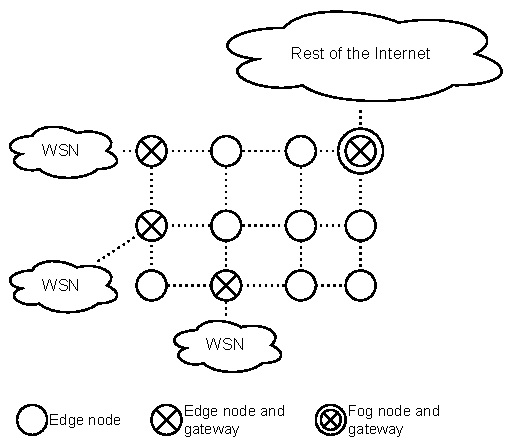
\includegraphics{problemStatementGeneral.pdf}
  \caption{An example of an IoT environment.}
  \label{problemStatementGeneral}
\end{figure}

The following simplifying assumptions are also made:
\begin{itemize}
 \item A DBMS instance can be installed on each of the edge nodes. A DBMS instance at a node enables the node to participate in query processing.
 \item Gateway nodes are more powerful nodes and always have a DBMS instance. Gateway nodes also have a database for persistent storage.
 \item The fog node is the most powerful gateway node and has always a DBMS instance. At least this node receives queries from any other node in the surrounding network or, for example, from the remote cloud. For the first evaluation it is sufficient if the fog node always performs the preprocessing of the query with a translation into an operatorgraph.
\end{itemize}
Based on these assumptions, three cases of the possible distribution of data storage and query processing are determined. Table~\ref{table_concept_cases} shows the possible cases. These cases can compete against each other in a simulation. A comparison of network overhead and energy consumption should provide information on how the deployment of DBMS instances is optimal.
\begin{table}[htpb]

  \centering
  \begin{tabular}{c|c|c}

      & \uzlemph{Centralized Storage}
      & \uzlemph{Distributed Storage} 
      \\ \hline
      \rotatebox[origin =c]{90}{\uzlemph{Centralized Processing}}
      &  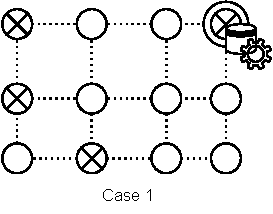
\includegraphics[valign=m,margin=0cm .2cm,scale=1.2]{figure_table_case1.pdf}
      & 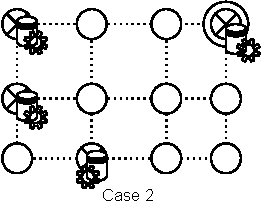
\includegraphics[valign=m,margin=0cm .2cm,scale=1.2]{figure_table_case2.pdf}
      \\ \hline
      \rotatebox[origin =c]{90}{\uzlemph{Distributed Processing}}
      &
      & 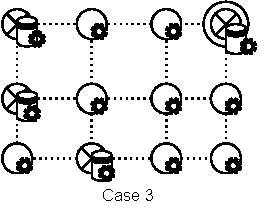
\includegraphics[valign=m,margin=0cm .2cm,scale=1.2]{figure_table_case3.pdf}
      \\ \hline
  \end{tabular}
  \centering
  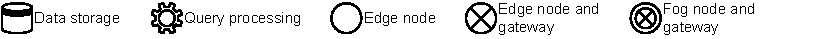
\includegraphics[valign=m,margin=0cm .5cm]{figure_concept-cases_legend.pdf}
  \caption{Three cases can be distinguished for the distribution of query processing and data storage.\label{table_concept_cases}}
\end{table}

The first case is a centralized data storage and a centralized query processing at the fog node. Sensors from the WSNs regularly send their samples to the fog node. The fog node receives a query about these samples and can complete the query processing. Processing is efficient because no additional network messages are required. However, it is questionable whether the efficiency of the query processing will compensate for the overhead of data transmissions from remote WSNs. The overhead caused by the transmissions increases in particular because, on the one hand, data is also sent that was not queried and, on the other hand, the edge computing capability of the intermediate nodes is not used to filter or aggregate the data.

The second case is a distributed data storage at the edge gateway nodes and a centralized query processing at the fog node. The sensors of a WSN use the nearest edge gateway node as a data sink. There is therefore an additional database for each WSN. The fog node receives a query and, during preprocessing, determines which databases need to be queried. In this case, only those data are sent over the network that are also requested in the query. In addition, the data sinks can participate in query processing to a locally limited extent. Filter or selection operators could be performed before the data is sent to the fog node. This case promises a smaller network overhead than in the first case.

The third case is a distributed data storage at the edge gateway nodes and a distributed query processing across all edge nodes with DBMS instance. The edge computing capability is fully exploited with the aim of reducing network overhead to a minimum. Compared to the second case, join operators can now also be carried out on intermediate nodes. Calculating joins as early as possible minimizes network overhead in the case of joins with no or few duplicates in the join attributes, which is a typical case in practice. In addition, the fog node is relieved of the query processing.

The centralized data storage and distributed query processing case will perform worse than the first case. Because for a distributed query processing, the data would first have to be distributed in order to later merge it again into an overall result. This case does not need to be evaluated.

\section{Example Scenario}
\label{section_Scenario}
For the evaluation of the protocol with a real DBMS, real data is also required, which is stored in the databases. Modeled sensors from WSNs serve as data sources. For the modeling, it is helpful to use a clear example scenario from practice. This makes the modeling more realistic and also easier to understand. Our example scenario is inspired from CityBench~\cite{CityBench}, which is a benchmarking framework for the evaluation of RDF stream processing engines with real smart city data sets. City Bench uses sensor data collected from the Danish city of Aarhus, where several smart city applications were used. One application of these is a parking space finder. Eight public parking lots in Aarhus were equipped with sensors that provided a continuous stream of data on parking space occupancy. A car driver could then, for example, submit a query to the IoT system for the next free parking space via a smartphone app.

A parking space finder is also used as an application example for the simulator. This example is simple, but still offers enough flexibility to model the various deployments of data storage and query processing in an edge computing environment. The university campus of L{\"u}beck is used as the observation area. Figure~\ref{figure_campus} shows the central part of the campus with ten marked parking garages. Each of the parking garages is covered by a WSN. In a WSN there is a sensor for each parking space that regularly detects whether its space is occupied or not. In order to allow more flexibility in the modeling, the static data sets from City Bench are not used. Instead, the sensors should generate their data themselves during the simulation runtime.
\begin{figure}[htpb]
  \centering
  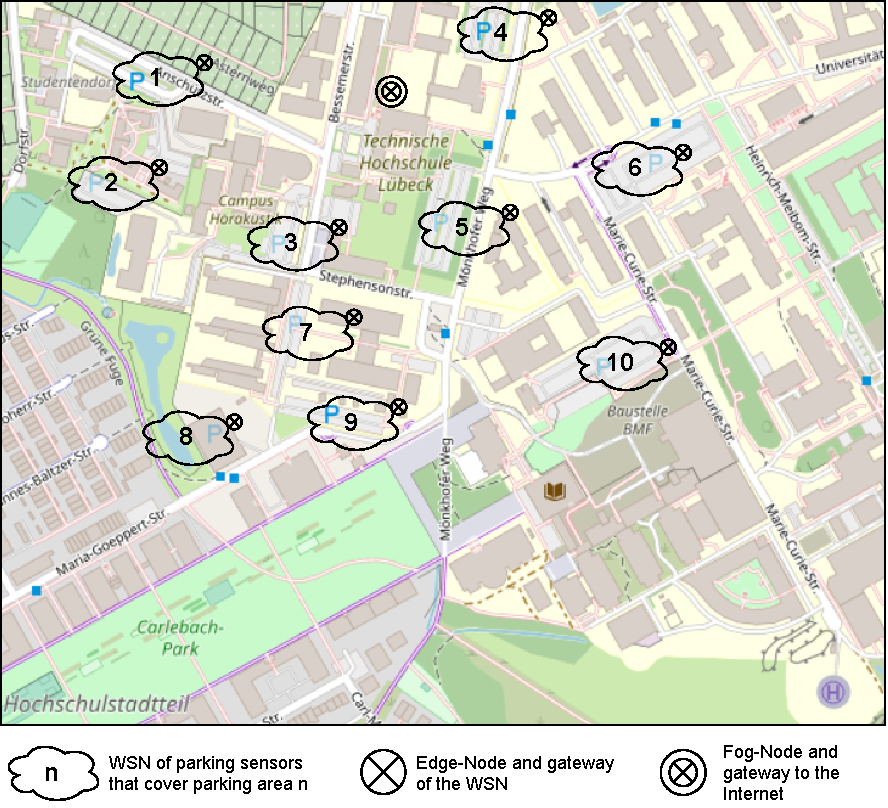
\includegraphics{campus.pdf}
  \caption{The university campus of L{\"u}beck serves as an area for the parking space finder application.}
  \label{figure_campus}
\end{figure}

In Semantic IoT, RDF is used as the basic data format. The samples from the sensors are first sent as binary raw data via the network to a data sink. Upon arrival, the Semantic Web DBMS instance encodes the raw data as RDF triples in order to save them in a triple store. In real applications, RDF triples are usually designed based on ontologies. For this reason, a SOSA-compliant format has been chosen for the simulator. An example sample is shown in Listing~\ref{sample_rdf}. This sample was sent from sensor number $2$ from parking area number $9$. It is the first sample of the sensor ($observation/1$). The sensor is located at parking space number $2$ and has recognized that the space is not occupied at the specified time.
\begin{SPARQL}[caption={Example of a sample in RDF.},
  float, label=sample_rdf, morekeywords={@prefix}, captionpos=b]
@prefix rdf: <http://www.w3.org/1999/02/22-rdf-syntax-ns#> .
@prefix xsd: <http://www.w3.org/2001/XMLSchema#> .
@prefix sosa: <http://www.w3.org/ns/sosa/> .

<http://observation/1/sensor/9/2> rdf:type sosa:Observation ;
sosa:hasFeatureOfInterest <http://parkingArea/9> ;
sosa:observedProperty <http://parkingSpace/2> ;
sosa:madeBySensor <http://sensor/9/2> ;
sosa:hasSimpleResult "false"^^xsd:boolean ;
sosa:resultTime "2021-06-09T15:41:01"^^xsd:dateTime .
\end{SPARQL}

Each sensor from each WSN periodically sends samples to a data sink at adjustable time intervals. Only such RDF triples are stored in the database of the sink. For the sake of simplicity, it is assumed that each parking space is monitored by exactly one sensor. Further data are not required for the evaluation of the protocol. 
A number of useful SPARQL queries can already be formulated with these triples.
For example, the number of currently free spaces in a certain parking area is of interest. The SPARQL query for this number is shown in Listing ~\ref{sparql_query_usecase}.
In the example, the number of free spaces in the parking area $9$ is queried. In order to get the current value of a sensor, all observations of the sensor made to date are aggregated in the subquery. The aggregate function $max$ is applied to the timestamp to get the maximum (most recent) value.

We offer a total of 8 queries with which the simulator can be tested. There are useful queries for the parking space finder application as well as queries which serve more for the purpose of evaluation. Further queries are listed in the Appendix~\ref{appendix_queries}.

\begin{SPARQL}[caption={Example of a SPARQL query that could be sent to a DBMS instance.},
  float, label=sparql_query_usecase, morekeywords={@prefix}, captionpos=b]
PREFIX rdf: <http://www.w3.org/1999/02/22-rdf-syntax-ns#>
PREFIX xsd: <http://www.w3.org/2001/XMLSchema#>
PREFIX sosa: <http://www.w3.org/ns/sosa/>

SELECT (count(?sensor) as ?numberOfFreeSpaces)
WHERE {
 ?o a sosa:Observation ;
 sosa:madeBySensor ?sensor;
 sosa:hasFeatureOfInterest <http://parkingArea/9>;
 sosa:hasSimpleResult "false"^^xsd:boolean;
 sosa:resultTime ?lastObservedAt .
 {
   SELECT(MAX(?d) AS ?lastObservedAt) ?sensor WHERE {
     ?o2 a sosa:Observation ;
     sosa:madeBySensor ?sensor;
     sosa:hasFeatureOfInterest <http://parkingArea/9>;
     sosa:resultTime ?d .
   }
   GROUP BY ?sensor
 }
}
\end{SPARQL}

\section{Modeling}
The simulator is designed as a DES system. DES systems inherently have a framework character in which the entities are controlled by the event-driven core. The modeling of the edge computing environment is based on the entities and events of the DES.
\subsection{Modeling the Network}
A flexibly configurable network of nodes and links is required for the simulator. The nodes have a position and can exchange network packets with several other nodes via links. Geographic coordinates (latitude, longitude) are used for positioning in order to satisfy the application example. For example, the edge gateway nodes of the WSNs can be assigned to real existing parking areas. A link can be modeled by specifying two nodes, a data rate, a maximum distance and a name that can be interpreted as a link type. The link type is used to check compatibility when linking nodes. For example, it can be used to model that a simple sensor only supports the abstract link type $A$, while an edge node supports the types $A$ and $B$. If the distance is small enough, then the sensor and the edge node can be connected via a type $A$ link.

For the modeling of larger networks, manual configuration at each individual node and link becomes time-consuming. Therefore, the option of automatically generated (sub-) networks is also required. These can cover a large area on the map with linked nodes of a node type. For the campus use case, a grid-shaped topology is needed, which is placed over the area of the campus. Manually configured, fixed gateway nodes can connect via the automatically generated network if they support the same link type as the network. Network partitioning can thus be ruled out.
\subsection{Modeling the Computing Performance}
The IoT is typically characterized by a high degree of heterogeneity in terms of computing resources. In order to allow different modeling, all types of devices from the computing pyramid must somehow be taken into account. Ideally, the performance of each modeled device can be configured before the simulation. The performance level serves as the basis for calculating the simulation time. Tasks that a device takes on require a certain processing time, depending on its performance. This duration is added to the simulation time. In a DES, the task of an entity is to process incoming events. Transferred to the IoT simulation, the task of a device is to process network packets.

The CloudSim-based simulators use \emph{million instructions per second} (MIPS) as a metric for performance. The MIPS is set for each modeled device in a configuration file. The tasks to be performed are modeled abstractly with an indication of the required number of instructions. The processing time of a task on a device is then obtained by simply dividing it with the MIPS. Provided that the storage hierarchy with the number of required disk accesses is also modeled, the determination of the processing time can be sufficiently precise.

In this simulation, however, real data is to be executed with real database operations. The processing time depends on the computer on which the simulation is running. When a modeled device receives a network packet, the current system time is recorded with $timestamp_{start}$.
As soon as the device has finished processing the packet and the transition to the next device is imminent, a second time stamp $timestamp_{end}$ is recorded. The processing time $timestamp_{end} - timestamp_{start}$ is the time that the simulation computer needed. This must be mapped to a simulated processing time of the simulated device.

One method would be to determine the MIPS of the simulation computer and then to compare it with the modeled MIPS of the device. This method may be sufficient for modeled computing tasks, but MIPS are unacceptable as a metric for real-world tasks. MIPS are only suitable for comparing processors and only if the processors use the same architecture~\cite{MIPS}. In addition, the determination of the disk accesses and a possible parallel execution of the simulation computer are insufficiently taken into account.

Another idea is to use a synthetic performance benchmark~\cite{MIPS}. This could be carried out in advance on the simulation computer. The results can be recorded in the configuration file together with the estimated (fictitious) results of the modeled devices. However, these results depend on the performance of the benchmark and can also be incorrect. In particular, they can be wrong for the modeled devices.

A better idea is to scale the execution time from the simulation computer by a percentage. In the configuration file, the performance on each device is specified with a percentage in relation to the simulation computer. The simulation computer always has a performance level of 100\%. A device that should only be half as powerful, for example, is configured with 50\% performance level. Of course, the scaling is only a rough approximation. However, provided that the modeled device has a similar computer architecture to the simulation computer, this method is sufficiently accurate. The simulated processing time of a network packet is then calculated using rule of three inverse with $(timestamp_{end} - timestamp_{start}) \times 100 \div level$. The level in percent is configured individually and in advance for each device.
\subsection{Modeling the Network Delay}
The network delay of packets must be modeled in a suitable way. Network packages in the IoT simulator are the events in DES that are assigned by entities to entities. The delays take up a significant proportion of the total simulation time, because a large number of packages are sent in a simulation run. In addition, many nodes usually take part in the transmission as hops between senders and receivers. The packets have real data as their payload, some of which can differ significantly in size. There are routing control packages for setting up the DODAG, sensor packages with raw sample data as well as various database packages with, for example, intermediate results from query processing. The latter tend to be larger.
The network delay from one hop to the next comes from four sources, which are called nodal processing delay, queueing delay, transmission delay and propagation delay~\cite{Kurose}.
\begin{description}
 \item [Nodal Processing Delay] is the time it takes for a node to examine a packet for bit errors and then to queue it up on the output link~\cite{Kurose}. This time depends on the computing performance. With specialized routers it is only a few microseconds~\cite{Kurose} and can be neglected for a simulation of such routers. In the IoT, the delay may be relevant~\cite{RPLEndToEndEstimation}.
 \item [Queueing Delay] is the time a packet spends in the queue on the output link~\cite{Kurose}. The queue serves as a buffer for traffic jams and to regulate the different working speeds of the network components.
  \item [Transmission Delay] is proportional to the packet size. It is the time to push all the bits of the packet into the output link~\cite{Kurose}. The bandwidth of the output link must be taken into account. This time is calculated with the packet size in bits divided by the data rate of the link in bits per second (bps)~\cite{Kurose}.
  \item [Propagation Delay] is the time it takes for a bit to travel up the link to the next hop~\cite{Kurose}. The speed at which a bit travels depends on the physical properties of the link and is in the range of 200 million to 300 million meters/second~\cite{Kurose}. The propagation delay is calculated as the distance in meters divided by the speed.
\end{description}
The total network delay results from the sum of the four delays. The calculation is even easier in the simulation. The nodal processing delay and the queuing delay are already covered by the calculation of the processing time with reference to the computing performance. The queue of network packets (events) for all devices is secretly managed by the DES scheduler. If several packages reach a device with the same arrival time, the device is called up several times in a row for processing. The propagation delay does not need to be calculated for the simulation, since its share in the total delay in a LAN is negligibly small. For example, at a distance of 5 km at the slowest speed, the delay is only 0.025 ms.

The transmission delay, on the other hand, makes up a large proportion of the total delay. In the simulation, the payload of the packets is coded as byte arrays. The size of the payload can thus be determined trivially. The IPv6 header of 40 bytes is used as the header size for all packets. For the sake of simplicity, there is no modeling of different link layer headers or possible compression mechanisms such as 6LowPAN. 6LowPAN would compress the IPv6 header down to 2 bytes~\cite{rfc4944}, but then the time for the (de)compression would also have to be modeled explicitly. These subtleties would only contribute slightly to the accuracy of the simulation result. The significant part is the payload as well as the data rate. To model the link layer, it is sufficient to specify a data rate in kilobits per second (kbps).

The simulated delay between receiving and processing a packet at node A, and sending it to node B is calculated as follows:
\begin{align}
  processingTime_A = (timestamp_{end_A} - timestamp_{start_A}) \times 100 \div level_A
\end{align}
\begin{align}
  transmissionTime_{A2B} = \frac{toKBit(header + payload)}{dataRateOfLink(A, B)}
\end{align}
\begin{align}
  totalTime = processingTime_A + transmissionTime_{A2B}
\end{align}
The $totalTime$ is also the delay given to an event in DES.

\section{Protocol Design}
The protocol design for distributed query processing is intended for a distributed DBMS whose instances are scattered across an IoT network. It is assumed that every instance knows the network address of every other instance or can determine it if necessary. It is also assumed that each instance knows the storage location (instance) of a data object in the form of a network address.
For example, if an instance receives a query in the form $Select\; x\; From\; A$, then the instance can resolve the query in the form $Select\; x\; From\; addressOf(A)$, where $addressOf(A)$ returns a valid address, to which a network packet can be sent. With these assumptions a protocol design for P2P-DBMS is pursued. With LUPOSDATE3000, addressing is implemented using a global hash table. Each DBMS instance has such a table. Global means that there is a table entry for every other instance and its stored data objects. An alternative to the global hash table would be a distributed hash table.

Given these assumptions, the distributed query processing requires a close interaction between the routing and the DBMS instances. That means, this protocol counts as in-network query processing protocol. The basic idea is to put the optimized operator graph of the query in the sink tree of the routing. The root of the operator graph and the root of the sink tree are the same DBMS node. However, a node in the sink tree do not necessarily correspond to exactly one data node of the operator graph. Several data nodes can be mapped to the same node in the sink tree. This is the case when the DBMS instance of a node stores the data that is also required by several operands (leaves) of the operator graph.

\subsection{Multicast Tree}
A node that receives a query first translates it into an optimized operator graph. The next step after translation is to send the operator graph to the DBMS nodes that contain the data of the operands for further processing. However, the operator graph is not sent as a whole to each of these nodes, because the DBMS nodes can only calculate a small part of the graph anyway. The operator graph is broken down into graph parts. A multicast is used to send the operator graph parts. The set of operands in the operator graph results in a set of destination addresses. The corresponding graph parts are sent to these addresses. The outward routes of the packets to these addresses span a tree that is a subtree of the sink tree. This tree is called a multicast tree.

The idea of the query processing protocol is that the operators of the operator graph are calculated on the way back from the leaf nodes to the root. In this sense, there is a multicast on the way there and a reverse multicast on the way back.

\subsection{Map Operators onto Multicast Trees}
The task of the query processing protocol is to map the optimized operator graph to a multicast tree. The mapping of root and leaf (operand) nodes is already given with the multicast tree. The main challenge now is to map the inner nodes of the operator graph to nodes in the multicast tree. Inner nodes are the operators (join, selection, etc.) that must be executed on the DBMS nodes between the leaf nodes and the root node. This mapping must meet the following three requirements (listed by priority $1 > 2 > 3$):
\begin{enumerate}
 \item The order of the operators in the operator graph must be maintained to ensure correct processing.
 \item The resources of the DBMS nodes must be taken into account, because in the IoT it may not be possible for every node to execute every operator.
 \item The operators should be executed as early as possible in order to keep the intermediate results to a minimum. For this purpose, a node that is closer to the leaf is preferred.
\end{enumerate}
Figure~\ref{figure_multicast_tree} illustrates the mapping. A sink tree is given with node $B$ as the root. $B$ receives a query and translates it into an operator tree. $B$ determines the destination addresses of the leaf nodes and sends a multicast. The multicast creates a multicast tree (marked in blue). The data is fetched from the leaf nodes and calculated on the way back to $B$ according to the operators from the operator tree. The protocol must define the multicast functionality with the required message types and the mapping of the operator graph to the multicast tree.
\begin{figure}[htpb]
  \centering
  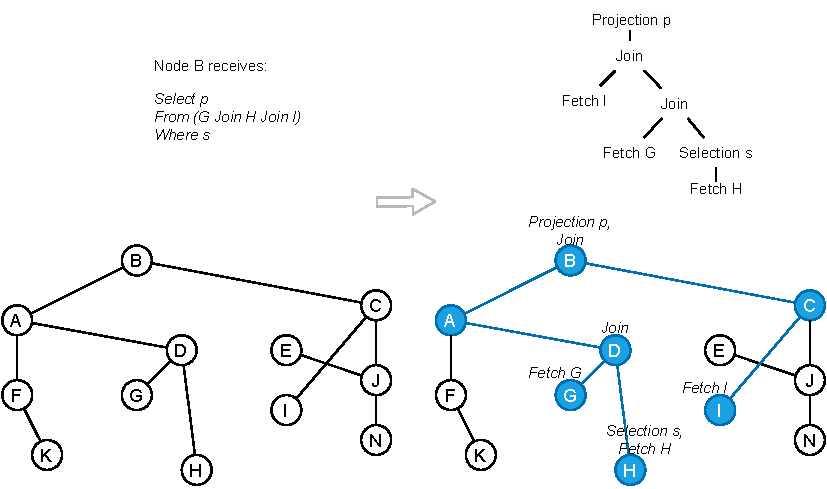
\includegraphics{figure_multicast_tree.pdf}
  \caption{Example mapping of an operator graph of a query to a multicast tree (marked in blue).}
  \label{figure_multicast_tree}
\end{figure}

One difficulty in mapping the operators to the nodes is taking dependencies into account. Some operators such as joins are dependent on two or more operands. This means that they cannot be executed until the data from the operands has been received. Such operators can only be carried out on common parent nodes of the operands. There are basically two approaches to finding these common nodes and assigning the operators to these nodes: a centralized or a distributed approach.

\subsection{Centralized Mapping Approach}
The common nodes can easily be calculated from a global perspective. Assume that the function $Path (X)$ returns the set of all nodes on the path from the root node to the node $X$. Then the set of common nodes between the two destinations $A$ and $B$ is equal to $Path(A) \cap Path(B)$. This calculation could only be carried out by a root node with global knowledge of all destinations including the complete paths to the destinations. This knowledge is present with routing protocols that use source routing. In the IoT domain, for example, there is RPL in non-storing mode.
\begin{figure}[htpb]
  \centering
  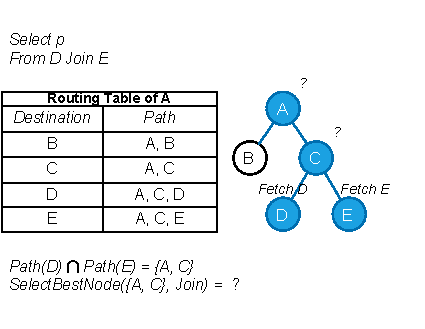
\includegraphics[scale=1.1]{figure_centralized_approach.pdf}
  \caption{Once the common nodes have been identified, a choice must be made for the join node in the multicast tree (marked in blue).}
  \label{figure_centralized_approach}
\end{figure}

After calculating the common nodes, the next step is to select a node as the operator node. A function $SelectBestNode (P, \varphi)$ is required, which selects the best node for the operator $\varphi$ from a set of common nodes $P$. An example for clarification is shown in Figure~\ref{figure_centralized_approach}. In this example, node $A$ receives a simple query. $A$ has global knowledge and can easily determine the common nodes of the required destination nodes $D$ and $E$.
The question now arises as to which node should be the join node.
The answer depends on whether logical operators or already physical operators are to be mapped to the nodes. For the mapping of physical operators, $A$ needs current knowledge about the state (e.g. energy) as well as about the fulfillment of necessary requirements (e.g. memory) of all other nodes. This information cannot be kept up-to-date without regular exchange. Regular exchange is problematic in constrained networks. If logical operators are mapped, then $A$ does not need to know the internal states of the potential join nodes. After the mapping, the join nodes themselves select the appropriate physical operator according to their internal state. Nevertheless, there is the problem of using a central component in a distributed system. Node autonomy and reliability can be better achieved with a distributed mapping without central knowledge.

\subsection{Distributed Mapping Approach}
In this thesis, the distributed mapping of operators to the nodes without global knowledge is implemented. Each DBMS node should decide for itself whether an operator can be calculated or not. The idea of determining the common nodes is based on the fact that branches in the multicast tree already mark common nodes. All nodes before a branch are common nodes for the subsequent nodes in the branches. Common nodes can execute operators like joins with multiple operands in which the operands are previously collected from the branches. For this purpose it is important that a node knows which operands can be expected from subsequent nodes. A multicast package provides the solution for this. The multicast is not implemented with many unicast messages. Instead, a packet is traversed on common paths until it is branched off. At the junction, the package is split and the parts for each branch are repackaged accordingly. The implementation of the multicast is part of the query processing protocol.

A set of operator graph parts and a set of destination addresses are part of every multicast package. The destinations are the leaf nodes of the multicast tree with the DBMS instances that have stored the data for the operator graph. A DBMS node can determine from each of the operator graph parts which dependencies exist on other DBMS nodes. For example, if a node determines that there are no dependencies for an operator graph part, the node can compute the operator graph part itself. In this case, all necessary data (operands) are available to calculate the operators from the operator graph part. If, on the other hand, data is missing from a data node, that is, there is a dependency on the data node, then data packets from this node must first be waited for.

If a DBMS node receives a multicast packet, it can determine which operator graph parts can be calculated directly. The result of the calculation then replaces the operator graph part. Usually, no calculations are carried out on the way to the leaf nodes, since the data must first be fetched from the leaf nodes. However, in this case the node can already decide for itself whether the operators can be calculated from an operator graph part even with resolved dependencies. In making this decision, the node takes into account its current physical resources. If the decision is positive, the node can enter itself in a list of DBMS nodes, which can also be included in the package. The list contains all addresses of DBMS nodes that are potential participants in query processing. These addresses are relevant for the way back from the leaf nodes to the root node. The root node is always the first participant in the list.

If a package is split due to a junction, the contents of the package are also split accordingly. The destination sets in each of the sub-packages are smaller. There are only those destinations left that can also be reached with the corresponding branch. This reduction is necessary so that subsequent DBMS nodes on the branches know from which destinations they can expect data. In addition, only the operator graph parts are included in a sub-package whose calculations depend on these destinations. Also, information about the existence of other operator graph parts is necessary if it can not already be determined from the available parts. A DBMS node needs to know whether the available operator graph parts in the present package are complete. If the participant list is also included in the package, it is not split up but copied. The list of participants grows individually in each package because other DBMS nodes can be on the corresponding branch. Alternatively, the list of participants can be kept in the DBMS instances.

A node can use the routing protocol to determine when a packet needs to be split. Routing must have been carried out before query processing so that each node can access a ready-made routing table. A routing table offers the function $getNextHop(dest)$, which returns the next hop in the sink tree to a destination. This function is called for all destinations in order to determine the set of next hops. There are so many sub-packages necessary as there are different hops. If the set contains only one hop, no splitting is necessary.

On the way from the root to the leaves, the packets may be split up several times. As soon as a leaf node is reached, the DBMS instance of the leaf node will be able to calculate at least one operator graph part. If there are no more operator graph parts to be calculated in the package and no further operator graph parts exist in other packages, the end result is available. The node can send the final result directly to the first participant on the list. Otherwise the node has only calculated an intermediate result. The intermediate result is sent to the last participant at the end of the list. The last participant is the DBMS instance that is closest. In the result package, information is also noted about which operator graph parts have been calculated or which operator graph parts still have to be calculated. The return path for this branch in the multicast tree is started with the result package.

A DBMS node that receives a result package tries to calculate the operator graph parts that are still open or to initiate their calculation. If all the necessary intermediate results are not available, a direct calculation is not possible. The node must decide whether the packet should be sent to the next participant or whether the necessary intermediate results from other branches will arrive at a later point in time. If further intermediate results are expected, the node can wait for their arrival. To do this, a node must recognize whether it is a common node of the other branches. If it is a common node, the path of the intermediate results of the other branches inevitably leads through this node. This requires information about the position in the multicast tree at which the split took place. If the currently present packet was split before the node, the node is not a common node of the branches. Correspondingly, the arrival of further intermediate results from other branches can be excluded. However, if the split has taken place on the node itself or on a child node, further intermediate results can be expected. There are two options for implementation. Either this information is in the package or the node stores this information itself.

The first option is that the split of a package is noted in all sub-packages on the way there. To do this, the address of the node that performed the split is written into each packet. On the way back, participant nodes can then use this address to determine at which position in the multicast tree the splitting took place. In addition, the remaining destination set is not discarded when splitting, but is stored separately in the package. This means that in addition to the set of destinations to which the package is directed, the other set of destinations is also present in each package. The other destinations are used to determine the splitting node with the help of function $getNextHop(dest)$ from the routing table. Suppose a node $K$ would like to determine for a received result packet whether further result packets from other senders will arrive at a later point in time. Then $K$ calls the function of his routing table for every other destination from the result packet. If at least one function call leads to a hop that is the parent of $K$, then $K$ cannot be a common node. The prerequisite is that a node can recognize whether a hop is the parent node. This is already the case with RPL, for example. Otherwise the routing protocol can also be adapted accordingly.

The second option is to save some data on the nodes.
A node saves that it has split a packet. In this case, the query processing protocol works in a stateful manner. The participant list, the other target sets and the position of the split can be saved at the node. This relieves the network traffic, but node failures or route changes lead to a restart of query processing. A distinction can be made between whether each node or only DBMS nodes save states. If every node is to save states, then every node must also implement the query processing protocol in its network stack. Storage space is also required, which can be a problem for some constrained devices. If only DBMS nodes store states, only such DBMS nodes have to implement the protocol and provide storage space. DBMS nodes are always powerful enough for this. In addition, this variant is more robust because the number of nodes with states is reduced to DBMS nodes. A failure of non-DBMS nodes can be tolerated if the routing protocol quickly provides an alternative route. One disadvantage is that the routing protocol has to be extended. In addition to the function $getNextHop(dest)$, there must be an extended function $getNextDatabaseHop(dest)$. This function returns the next hop with DBMS instance on the route to the destination. The reason is the special case that there can be a junction at a node that does not have a DBMS instance. Figure~\ref{figure_nextDBHopFunc} shows an example of this. The DBMS node $A$ must already perform the split before the junction at $B$ in order to reach the DBMS nodes $C$ and $D$. $getNextHop(dest)$ is no longer sufficient to decide whether a package needs a split.
\begin{figure}[htpb]
  \centering
  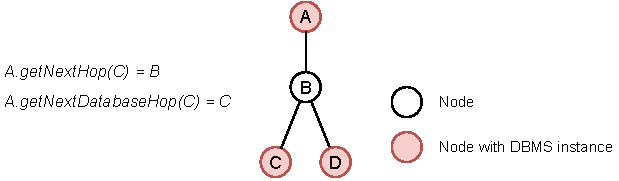
\includegraphics[scale=1.1]{figure_nextDBHopFunc.pdf}
  \caption{Example of a junction at a non-DBMS node.}
  \label{figure_nextDBHopFunc}
\end{figure}

With both the stateless and the stateful option, query processing can be divided into two phases. The first phase comprises the way of the network packets from the root to the data nodes. In this phase, the query processing is only prepared. The second phase involves the way of the packets from the data node to the root. The actual query processing takes place on the way back. The two phases are compared in Table~\ref{table_query_processing_phases}.
\begin{table}[htpb]

  \centering
  \begin{tabular}{p{2cm}|p{6cm}|p{6cm}}

      & \uzlemph{First Phase: Way There}
      & \uzlemph{Second Phase: Way Back} 
      \\ \uzlhline
      \uzlemph{Purpose}
      & The participating DBMS instances are prepared and pre-selected.
      & All operators from the operator graph are calculated.
      \\[3ex] 
      \uzlemph{Package}
      & Multicast packets with operator graph parts are sent to a set of destination addresses.
      & Unicast packets with operator graph parts and / or (intermediate) results are sent to individual destination addresses.
      \\[3ex] 
      \uzlemph{Visit}
      & All DBMS instances on the multicast tree are visited.
      & A subset of all DBMS instances on the multicast tree are visited. The leaves and the root are always visited.
      \\[3ex] 
      \uzlemph{Fragmentation}
      & Packets may be fragmented on the way there. This only happens at the points where a junction is imminent and the targeted DBMS instances can only be reached via different paths. For determining whether a junction is imminent, the routing protocol must be consulted.
      & On the way back, packages are merged. This does not have to happen at the points where a junction has led to a split. It can also happen further up in the multicast tree between the junction and the root. The points of merge are the DBMS nodes that choose to calculate operators with multiple operands.
  \end{tabular}
  \centering
  \caption{Comparison of the two phases.\label{table_query_processing_phases}}
\end{table}
\subsection{Extension of the Routing Protocol}
An abstract implementation of a routing protocol is required in order to be able to simulate the in-network query processing. The choice falls on RPL. RPL is widespread in the IoT and is the de facto standard for LLNs~\cite{RPLApplications}. In principle, query processing can also be implemented with other routing protocols that enable routing with local knowledge. In RPL there is the storing mode for this. In this mode, each node builds up its local knowledge with its own routing table. For the evaluation it is sufficient if every node in the network is an RPL router of one DODAG. Only one DODAG is needed, which is automatically constructed after the simulation has started. Network packets with DIOs and DAOs are exchanged between the nodes. The fog and gateway node is the DODAG root. The OF for the rank calculation is based on the shortest distance and a variable $MinHopRankIncrease$ of $1$. This variable represents the minimum increase in rank~\cite{rfc6550}.

The extension of the routing protocol is the offer of a new function that returns the next hop with DBMS instance for a given destination address. Figure~\ref{figure_q_processing_stack} shows a section of the protocol stack with the function as a service for the query processing protocol. For the implementation of the function, a second table with destinations to next database hops is introduced in addition to the existing routing table with destinations to next hops. This table is also built up with the DAO messages. For this purpose, in addition to the destination set, a set of next database hops is also sent in a DAO. The sender also communicates with the DAO whether it owns a DBMS. A recipient can now take over the destinations as well as the associated database hops if the sender does not have a DBMS instance itself. Otherwise the sender replaces the database hops.

In addition, a DAO delay timer is used as suggested in the RPL specification~\cite{rfc6550}. This reduces the number of DAO messages. The delay time corresponds to the default value of 1 second.
\begin{figure}[htpb]
  \centering
  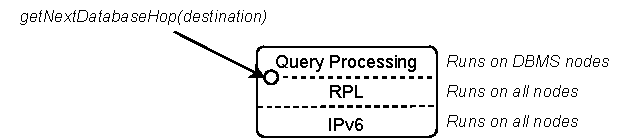
\includegraphics[scale=1.1]{figure_q_processing_stack.pdf}
  \caption{RPL offers a new service.}
  \label{figure_q_processing_stack}
\end{figure}

\chapter{Implementation}
\label{chapter_Implementation}
The realization of the simulator includes implementation and testing of three modules. Kotlin is used as the programming language in order to strive for multiplatform capability. The configuration of the IoT models is done in a JSON file. There is a total of 4664 source code lines, which are distributed over 78 Kotlin files\footnote{Measured on July 20, 2021}. Among these are 138 test cases. LUPOSDATE3000 is integrated as an external system. There are also two further dependencies on the external libraries \emph{kotlinx.serialization}\footnote{https://github.com/Kotlin/kotlinx.serialization} and \emph{kotlinx-datetime}\footnote{https://github.com/Kotlin/kotlinx-datetime}.
\section{Simulator Architecture}
The programming tasks can be broken down into three large sub-tasks, each of which can be developed in separate modules. Implementation and testing can be carried out separately for each module. The external system LUPOSDATE3000 is connected to the simulator via an interface. Figure~\ref{figure_architecture} shows the system design as a package diagram in \emph{Unified Modeling Language} (UML)~\cite{UML_Spec}.
\begin{figure}[htpb]
  \centering
  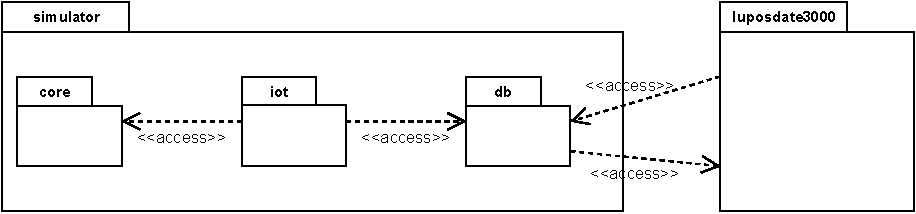
\includegraphics[scale=0.9]{figure_architecture.pdf}
  \caption{The simulator consists of three modules.}
  \label{figure_architecture}
\end{figure}

The first module called $core$ implements the discrete event-driven simulation in a general way. This means that the module can deliver the event-driven simulation for any problem domain. In this case, only IoT is needed. In addition, $core$ has no dependencies on other modules in the system.

The second module called $iot$ is the most extensive. It uses $core$ to simulate the IoT models. The models are generated when a configuration file is parsed. The visualization as well as the measurements during the simulation are carried out in $iot$. The starting point of the simulator is also located here.

The third module called $db$ contains the interfaces for integrating DBMSs. There is an interface for the DBMS to access the simulator and also an interface for the simulator to access the DBMS. In addition, a dummy DBMS implementation is provided for test purposes.

\section{Event-Driven Framework}
The UML class diagram of the $core$ module is shown in Figure~\ref{figure_des_classes}. The module is designed as a framework in which the simulation is event-driven. After the parameters have been transferred and the simulation has started, the simulation runs autonomously until the end. Below is a description of the classes that provide a detailed look into the implementation.
\begin{figure}[htpb]
  \centering
  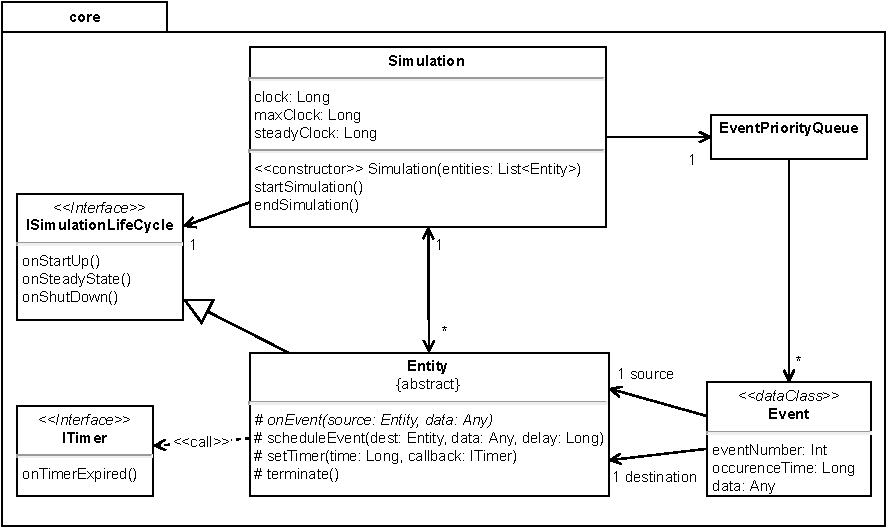
\includegraphics{figure_des_classes.pdf}
  \caption{Class diagram of the $core$ module with the essential elements.}
  \label{figure_des_classes}
\end{figure}
\begin{description}
\item [Event]
 is a simple data class without methods. In terms of event-driven simulation, an event is assigned from a source entity to a destination entity. A time of occurrence defines when the event reaches the destination for processing. An event always has data pending, which can be used for processing. To make the data transfer universal, the most general class type is used (It's \emph{Any} in Kotlin). A large number of $Event$ objects are typically generated in a simulation. Each $Event$ has a number for identification.
\item [EventPriorityQueue]
is a class that implements a priority queue for events. $Event$ objects are first sorted in descending order according to the time of occurrence, so that the head of the queue always has the smallest time. For events with the same time of occurrence, the event number is used as the second sorting criterion. The event with the smallest number is preferred because it was created first. In this way, the sequence of event processing is correctly adhered to.
\item [Entity]
is a class that implements a self-contained model of the system to be examined in the context of event-driven simulation. The class is abstract to allow universal modeling. All simulation-specific parts are hidden in the abstract class. The inheriting class can thus focus on the problem domain. Typically, the system is modeled by many entities that assign events to each other in order to cooperate. The $Entity$ class therefore has a method for assigning events and a method for processing assigned events. When making an assignment, a delay time is also specified. This time, added to the current simulation clock, results in the time of occurrence of the event at the target entity. In addition, a termination method is provided for premature termination of the entity in the simulation run. All assigned events after the termination time are no longer processed by the entity.
\item [ITimer]
is an interface that can be used by concrete $Entity$ classes to implement a timer mechanism.
An entity can also assign an event to itself to take some action after a certain point in time in the future. This procedure can be used to provide a kind of timer. For a convenient and universal timer implementation, the entity has a method with a parameter of the $ITimer$ type. The method secretly creates a self-event in which the $ITimer$ object is saved as the data of the event. After the delay time has elapsed, the callback method of the $ITimer$ object is called.
\item [ISimulationLifeCycle]
is an interface that specifies callback methods that indicate the current phase of the simulation run for the implementer. The simulation runs through the three phases start, steady and end one after the other. At the beginning of each of these phases, the corresponding method is called on the implementing object. The object could, for example, visualize the state or carry out other actions at the beginning of certain phases. $ISimulationLifeCycle$ is also inherited from the abstract $Entity$ class.
\item [Simulation]
is a class that manages the entire simulation run. During the run, an instance of $EventPriorityQueue$ is used to assign the events to the destination entities at the right time. All generated events are always sorted into this queue first.
Before the simulation run, at least a list of the participating entities is required. In addition, it can be set when the steady state and when the end state is reached. The default value for the steady clock defines that the simulation simply skips the steady phase. This can be useful if no such phase is needed in the modeling. The default value of the maximum clock means that the simulation will run until either there are no more events to process or the termination is explicitly initiated.
A method is provided for both starting and ending the simulation. In addition, the current clock can be asked at any time. Before the start of the simulation, the clock is always at $0$. During the simulation run, the clock is incremented in an event-driven manner. After the end, the clock remains constant at its final value. The methods for starting and stopping can only be called in this order and only once at a time. For a new simulation run, the class $Simulation$ must be re-instantiated.
\end{description}
\section{Database System Interface}
The connection to an external DBMS is defined using a small number of Kotlin interfaces and classes. These are located in the $db$ module. Figure~\ref{figure_db_classes} shows the class diagram for connecting including the required methods.
\begin{figure}[htpb]
  \centering
  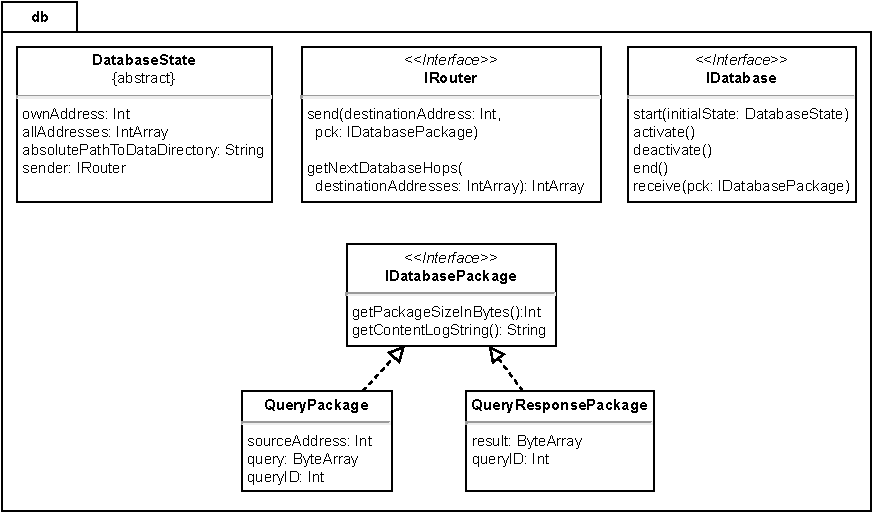
\includegraphics{figure_db_classes.pdf}
  \caption{Interfaces and classes for connecting to external DBMS.}
  \label{figure_db_classes}
\end{figure}
\begin{description}
 \item [IDatabasePackage]
 is an interface that can be implemented by all packets that are sent from or to DBMS instances. This includes queries and query results that are exchanged between the simulator and the DBMS. In addition, DBMS internal packages are required for coordination and query processing, which are sent between the DBMS instances. This interface creates a common denominator for these packages. A DBMS can define as many packages as it needs. The contents of the package remain hidden from the simulator. The simulator only needs two methods. For measurements of the network traffic, each packet must implement a method for returning the packet size in bytes. In addition, a method must be implemented which returns the package content as a string for logging.
 \item [QueryPackage]
 is a class that represents packets that can be used to send a query to a DBMS instance. Query strings will be encoded as a byte array. In addition, the address of the sender is required so that a response can be made. The response is defined with the $QueryResponsePackage$ class. An identification number is used for the mapping of query and query response. The query sender puts the number in the packet and expects a response with the same number.
\item [IRouter]
is an interface that is implemented by a class in the simulator and used by a class in the DBMS. The simulator thus offers a method for sending database packets. The destination address of the package must be specified for sending. The implementing class in the simulator can then use RPL to determine the next hop on the route to the destination. In addition, a method is offered for the query processing protocol that returns the corresponding set of hops with DBMS instance for a given set of destinations.
\item [DatabaseState]
is an abstract class that represents a state of the DBMS. States are used to simulate a set of DBMS instances. Only one real DBMS is integrated into the simulator, but several states are managed. The entire state of an instance is saved in a folder on the file system. As soon as a device decides to contact its instance, the corresponding folder is loaded into the DBMS. At any point in time in a simulation run, only one instance is active. This means that the folders are exchanged when the instances change\footnote{In LUPOSDATE300 only variables are exchanged. The states remain in the memory.}. The path is specified in the $DatabaseState$ object so that the DBMS can find the folder. A state includes the network address of its own device and the addresses of all other devices with a DBMS instance. In addition, a reference to the implementing object of $IRouter$ is saved.
\item [IDatabase]
is an interface that is implemented by a class in the DBMS and used by a class in the simulator. At the beginning of the simulation, each device with a DBMS instance calls the $start$ method in $IDatabase$ within its initialization phase. This method is used to initialize the DBMS instance. The initial state of the instance is transferred as a parameter. It contains the folder path to the newly created folder in the file system. The instance can be activated or deactivated during the simulation run. As soon as a device is instructed to process a network packet with database content, this device will activate its DBMS instance. The activation process loads the folder that contains the last state of the instance from the file system. The package is then transferred to the DBMS using a $receive$ method. In the context of the $receive$ method, the DBMS can call any number of send methods from $IRouter$. When the processing of the package is finished, the device calls the deactivate method so that the DBMS can prepare for a new change of state. At the end of the simulation, all states can be deleted by calling the $end$ method.
\end{description}
\subsection{Interface Usage}
Figure~\ref{figure_db_interface} shows the classes involved in the interface usage. From the simulator side, all interface dependencies are encapsulated in the $DatabaseAdapter$ class. A $Device$ object uses this adapter to communicate with its DBMS instance. $DatabaseAdapter$ implements the $IRouter$ interface and uses the $IDatabase$ interface. On the opposite side there are currently two DBMS implementations. 
A dummy implementation is used for test purposes and can be used as a template for real DBMS\footnote{For the sake of clarity, relationships of the $dummyImpl$ are not shown. However, these are similar to $luposdateImpl$.}. A real DBMS implementation is provided with LUPOSDATE3000. There is the $DatabaseHandle$ class as a central point of contact for this system. $DatabaseHandle$ implements the $IDatabase$ interface and uses the $IRouter$ interface. The abstract class $DatabaseState$ and the interface $IDatabasePackage$ are used by both sides.
\begin{figure}[htpb]
  \centering
  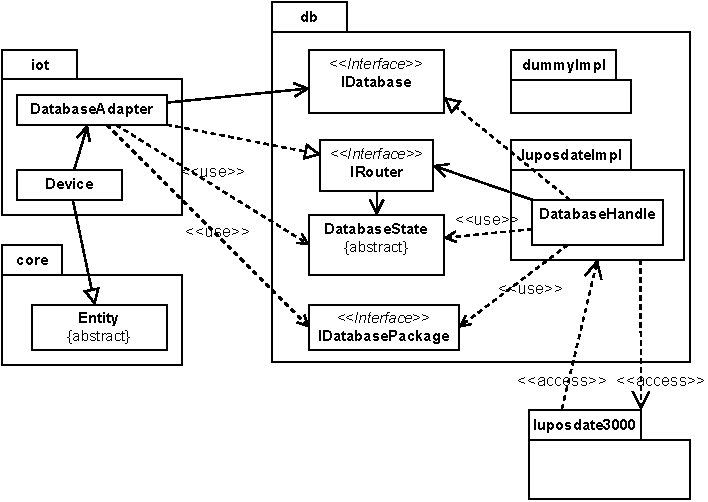
\includegraphics{figure_db_interface.pdf}
  \caption{Section of the system that shows the interface usage.}
  \label{figure_db_interface}
\end{figure}

\chapter{Evaluation}
The evaluation of this work is divided into three sections. First, the verification of the functional correctness is presented, as it was done during and after the development of the simulator. Next, the performance of the simulator is measured and presented. Finally, the query processing protocol is analyzed with the SPARQL queries in the example scenario.

The evaluation is carried out on a single socket machine with an Intel i7-6700HQ CPU and a clock rate of 2.60 GHz. There are 8 hardware supported threads and 8GB of installed RAM. The machine uses Java version 1.8.0. IntelliJ IDEA with 2048 MB maximum heap size is used for execution.
\label{chapter_Evaluation}
\section{Automated Tests}
The Kotlin test library were used to ensure the functional correctness of the simulator with automated tests. Every public method in the program code is covered by at least one test case. This small-step procedure corresponds to unit testing~\cite{BasisTest}. The unit tests were always developed parallel to the productive code and many program parts were also developed test-driven. Accordingly, the test code with 2098 lines of source code makes up about 55\% of the code base.

Figure~\ref{figure_evaluation_testSummary} shows the test summary. The test cases in the $core$ module are comparatively fast because they do not have to access the file system except for the log output. The tests of the $iot$ module are slower. These load and parse a total of 42 JSON configuration files in order to check various configuration options. The integration tests are by far the slowest. They verify the interplay between the simulator and LUPOSDATE3000. For the integration tests, among other things, the campus topology is checked with the 8 different SPARQL queries and several DBMS instances. In addition to using assert methods from the test library, the log messages of the simulator in debug mode are also used in the integration test.
\begin{figure}[htpb]
  \centering
  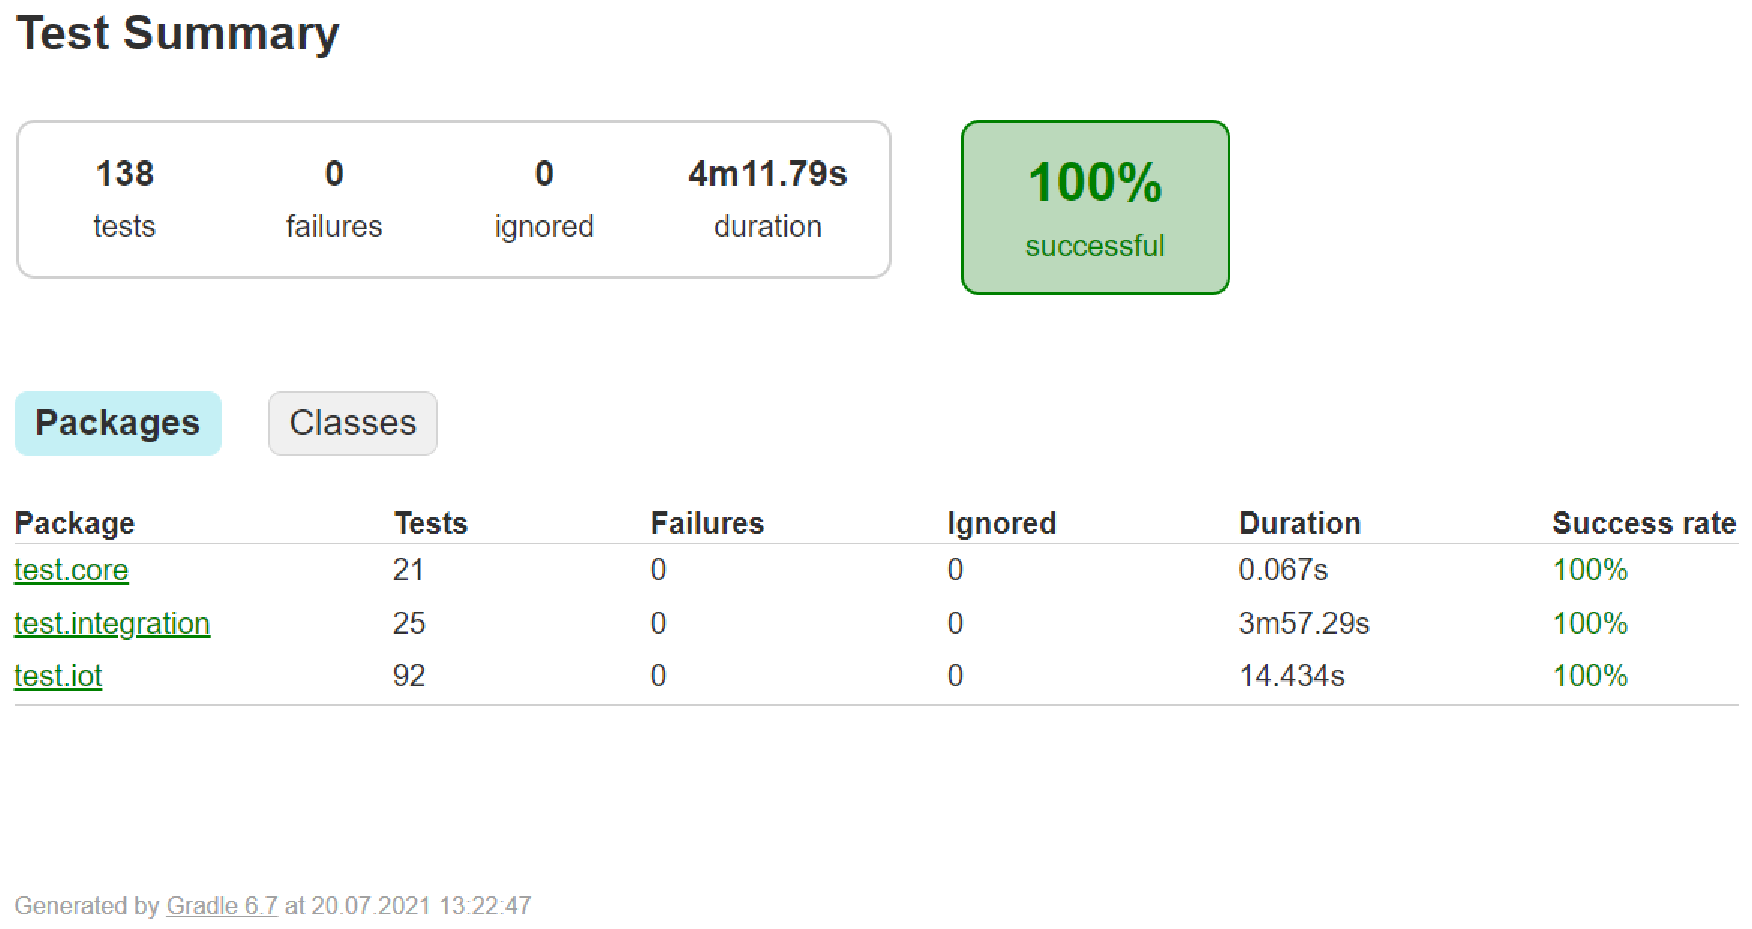
\includegraphics[scale=0.5]{figure_evaluation_testSummary.pdf}
  \caption{All tests are successful.}
  \label{figure_evaluation_testSummary}
\end{figure}

\section{Simulator Performance}
The simulator offers two basic topologies to model different networks. There is a star topology with a root node and directly connected child nodes. There is also a mesh topology to distribute nodes on a rectangular area in the landscape. In this section we analyze the scalability of the two topologies.

\subsection{Star Topology Scaling}
The star topology has one root node and $n$ child nodes. The child nodes are directly connected to the root and therefore there are $n$ links. With this topology, RPL causes minimal overhead in terms of the number of messages. The DODAG is fixed from the start. Only one DIO message and one DAO message are sent for each link and the network traffic remains small. The star topology is suitable for analyzing the scaling in number of devices (nodes). We compare the scaling for devices without a DBMS instance, with a dummy DBMS instance and with a LUPOSDATE3000 instance. All measurements are repeated $100$ times to present the average values with a smaller standard deviation.

A sequence of simulation runs is executed for the evaluation.
Starting with a root node in the first simulation run, a set of child nodes is added for each subsequent simulation run. The initialization duration and the real simulation duration are measured. The initialization begins with the parsing of the configuration file and ends as soon as the simulation framework calls the $onStartUp()$ method of its entities. Calling this method also starts the simulation phase. The simulation phase ends when the framework calls the $onShutDown()$ method.

Figure~\ref{figure_evaluation_starPerf_Without} shows the measurements for devices without a DBMS instance. On average, the standard deviation is 15\% for the initialization time and 46\% for the simulation time. The increasing distance between the two lines can be explained by the increasing number of RPL control messages and the growing routing table in the root node. The routing table has an array entry for each of the child nodes.
\begin{figure}[htpb]
  \centering
  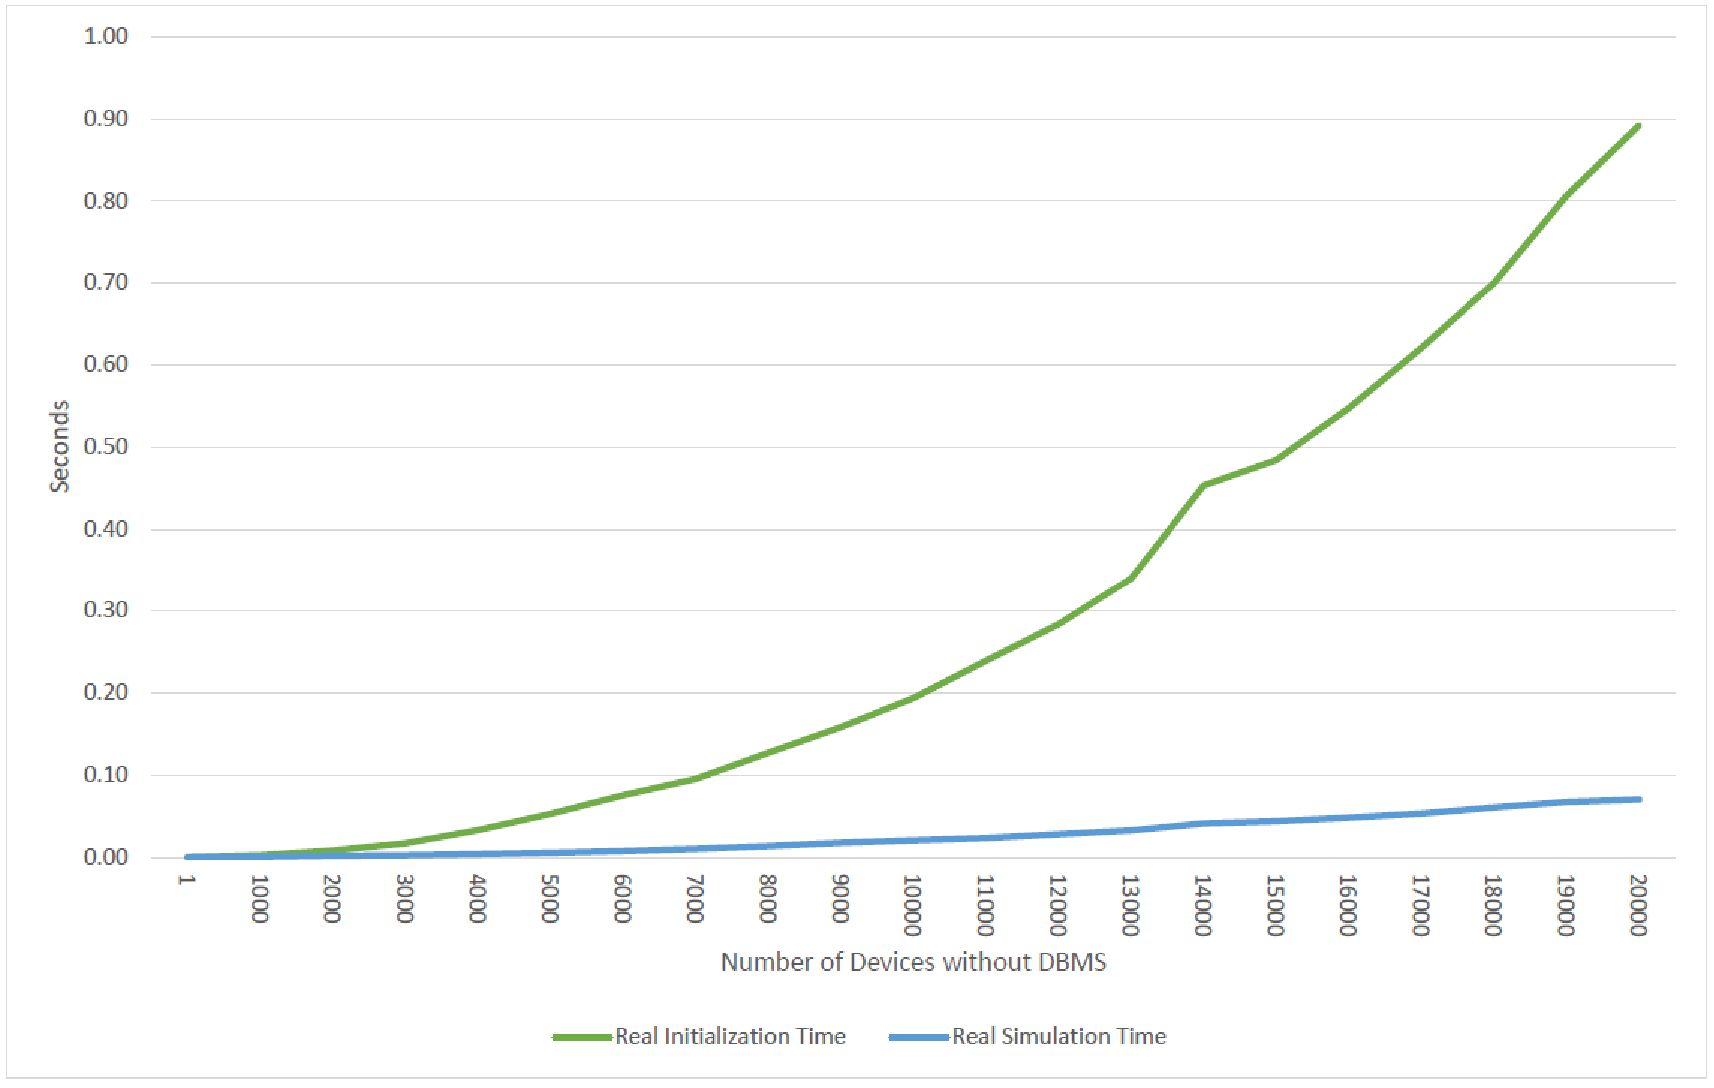
\includegraphics[scale=0.5]{figure_evaluation_starPerf_Without.pdf}
  \caption{Scaling in the number of devices without DBMS}
  \label{figure_evaluation_starPerf_Without}
\end{figure}


Figure~\ref{figure_evaluation_starPerf_Dummy} shows the measurements for devices with the dummy DBMS instance. The execution time is considerably longer because the file system is being accessed. Each device creates the folder for saving the database status during the initialization phase. In addition, a text file is stored in this folder by the dummy DBMS in the simulation phase. The standard deviation is therefore much higher with 63\% for the initialization and 66\% for the simulation.
\begin{figure}[htpb]
  \centering
  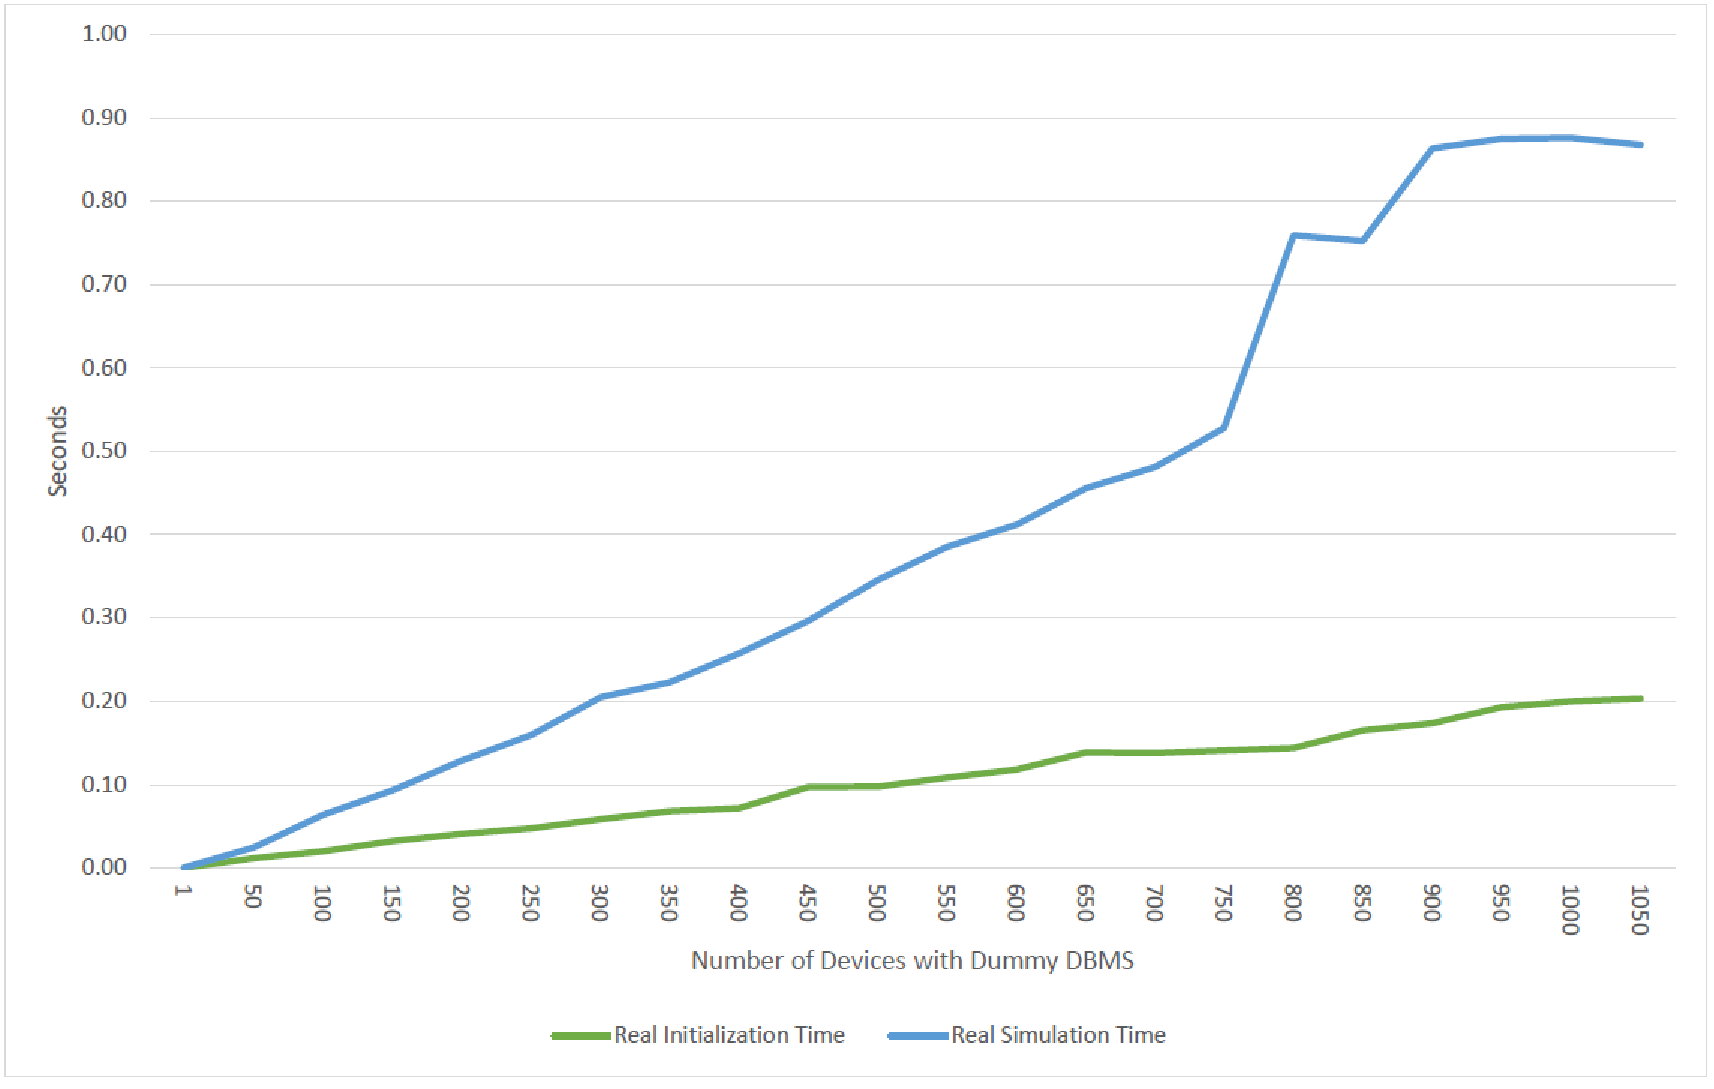
\includegraphics[scale=0.5]{figure_evaluation_starPerf_Dummy.pdf}
  \caption{Scaling in the number of devices with dummy DBMS}
  \label{figure_evaluation_starPerf_Dummy}
\end{figure}

In Figure~\ref{figure_evaluation_starPerf_Lupos}, the times for devices with the real LUPOSDATE3000 instances are measured. The average standard deviations are 88\% for the initialization period and 39\% for the simulation period. The steep increase in simulation times from around 1000 devices is probably related to the use of the heap memory. After 1171 devices there is a memory error with 2048 heap size.
\begin{figure}[htpb]
  \centering
  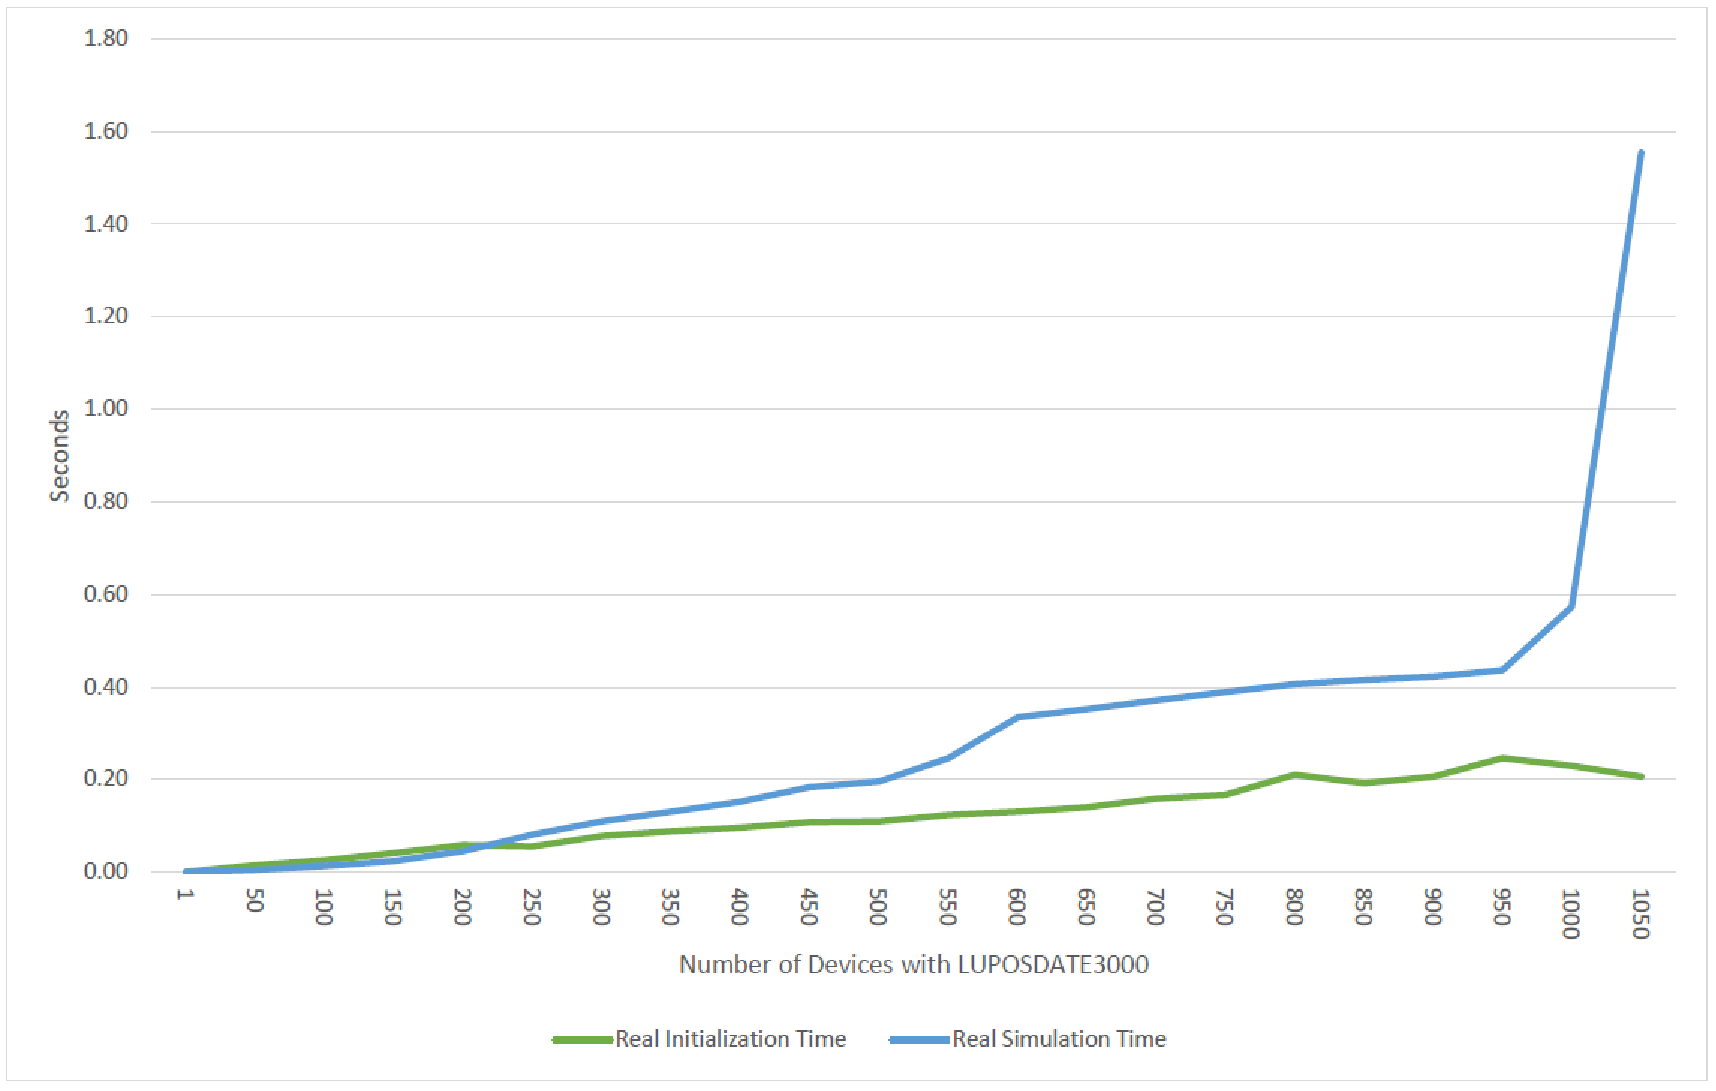
\includegraphics[scale=0.5]{figure_evaluation_starPerf_Lupos.pdf}
  \caption{Scaling in the number of devices with LUPOSDATE3000}
  \label{figure_evaluation_starPerf_Lupos}
\end{figure}

\subsection{Mesh Topology Scaling}
The mesh topology can be used to configure an area with complete signal coverage in order to avoid network partitioning. A mesh is specified in the configuration file with a start location for the first device and information about the length and width of the area. In addition, the protocol type of the devices is specified. During the parsing process, the simulator places new devices until the area is filled.
The signal range of the protocol type determines the distances between the devices. The mesh topology can therefore be scaled in two ways. On the one hand via the size information and on the other hand via the signal range. For the evaluation we use the campus map from the example scenario with a fixed predetermined area of $600 m^2$ and scale by specifying the signal range. The measurements start at a signal range of $600 m$ and are reduced by $30 m$ for each further simulation run. 

The measurements regarding the scaling in number of devices and links are shown in Figure~\ref{figure_evaluation_meshPerf_links}. The numbers increase significantly with a smaller protocol signal range. The simulation time also increases significantly with the number of links, because the devices have to send and process more RPL control messages.
\begin{figure}[htpb]
  \centering
  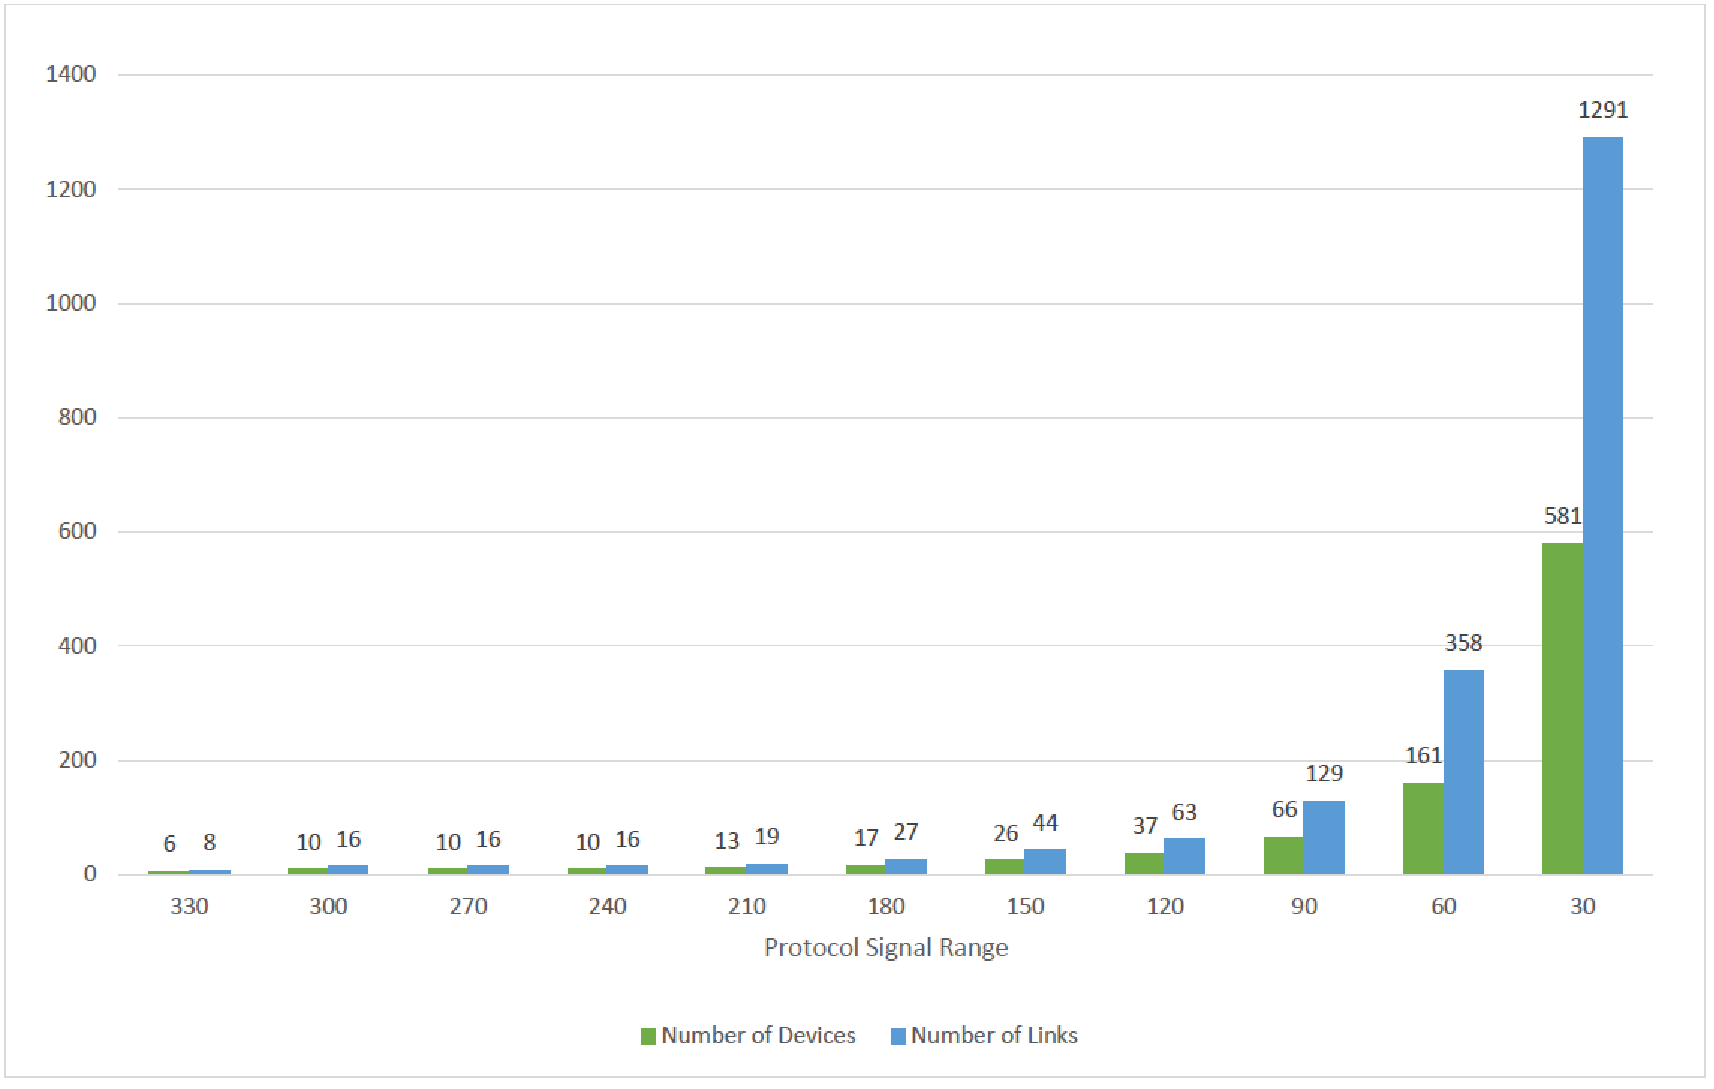
\includegraphics[scale=0.5]{figure_evaluation_meshPerf_links.pdf}
  \caption{A reduction in the protocol signal range in the mesh topology leads to a rapid increase in devices and links.}
  \label{figure_evaluation_meshPerf_links}
\end{figure}
\begin{figure}[htpb]
  \centering
  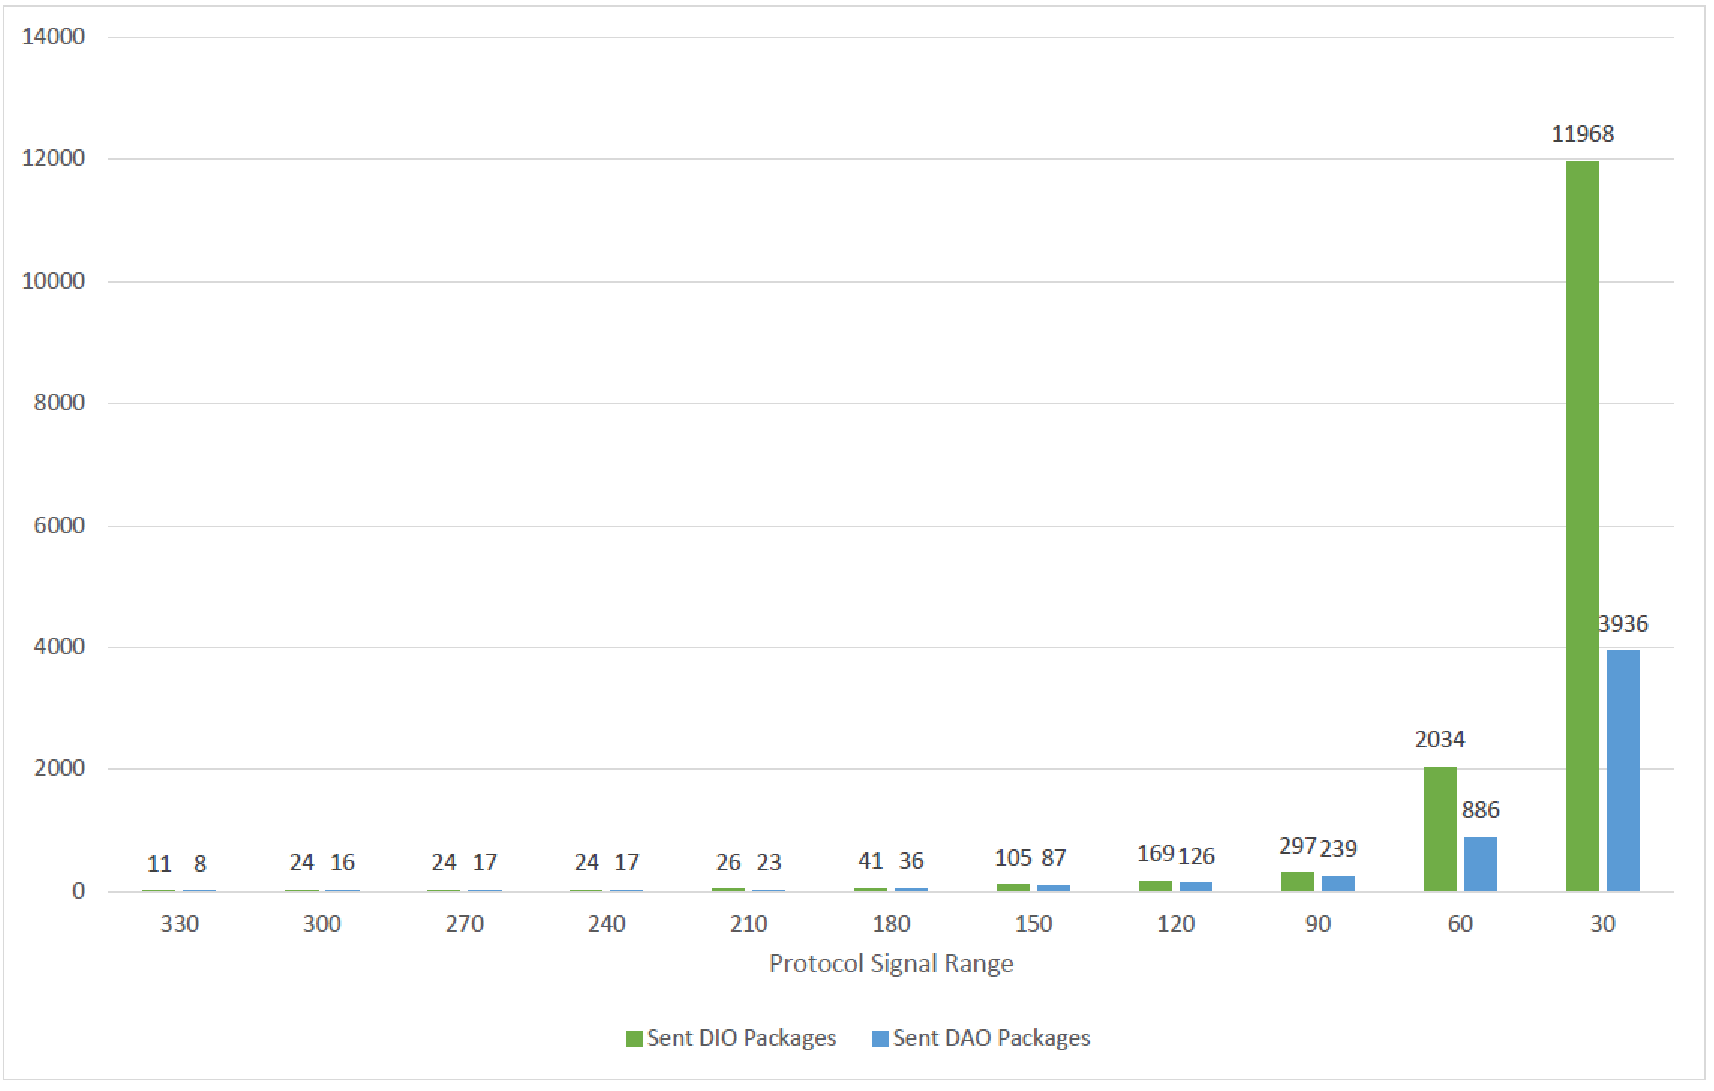
\includegraphics[scale=0.5]{figure_evaluation_meshPerf_time.pdf}
  \caption{A reduction in the protocol signal range in the mesh topology leads to a rapid increase in RPL control messages.}
  \label{figure_evaluation_meshPerf_time}
\end{figure}

Figure~\ref{figure_evaluation_meshPerf_time} shows the corresponding number of DIO and DAO packages sent. This exponential trend must be taken into account when modeling. The simulator performs explosively poorly on a tightly meshed network. For the modeling of such networks, an extension for parallel processing in the simulator should be considered.



\section{Protocol Analysis}
The goal of distributed query processing in edge computing is to reduce resource consumption. A significant part of the resource consumption arises from the necessary network communication with regard to the size and number of messages. We therefore examine distributed query processing in terms of these two parameters.
\subsection{Experiment Setup}
The basis of the experiment is the comparison between the cases as presented in Table~\ref{table_concept_cases} in Chapter\label{chapter_Concept}. Three cases were described that were derived from the distinction between query processing and data storage.
Due to the current development progress in LUPOSDATE3000, some adjustments to the case comparison are necessary. It is currently not possible to differentiate between processing and storage within a DBMS instance. Therefore, only a centralized case is compared with a distributed case.
\begin{description}
 \item [Centralized Case:]In the centralized case is only one node with DBMS instance, hereinafter referred to as the fog node, which carries out the processing and storage. All sensors from the WSNs use the fog node as a data sink.
 \item[Distributed Case:]  In the distributed case, each WSN has one edge node with a DBMS instance as a data sink and gateway. In addition to the WSNs, there is also the fog node with a DBMS instance. All instances participate in query processing.
LUPOSDATE3000 has currently no restriction to the local storage of data on one node. This means that the sensors send to an instance, but the instance then further distributes the data between all existing instances. The distributed case is therefore a complete distribution between query processing and data storage.
\end{description}

The parking space finder application presented in Section~\ref{section_Scenario} serves as the experimental scenario. There are a total of $10$ parking areas. Each parking area is a WSN, with one sensor placed on one parking space. A WSN is modeled with a star topology in the configuration file.
The root of the star topology is the edge and gateway node of the WSN. The fog node is firmly placed on the map as a stand-alone node. The fog node serves as the root for the DODAG and as the root for query processing\footnote{In the current implementation, any DBMS node can already take on these tasks.}.
The mesh topology is used to interconnect all gateway nodes and the fog node.
\begin{figure}[htpb]
  \centering
  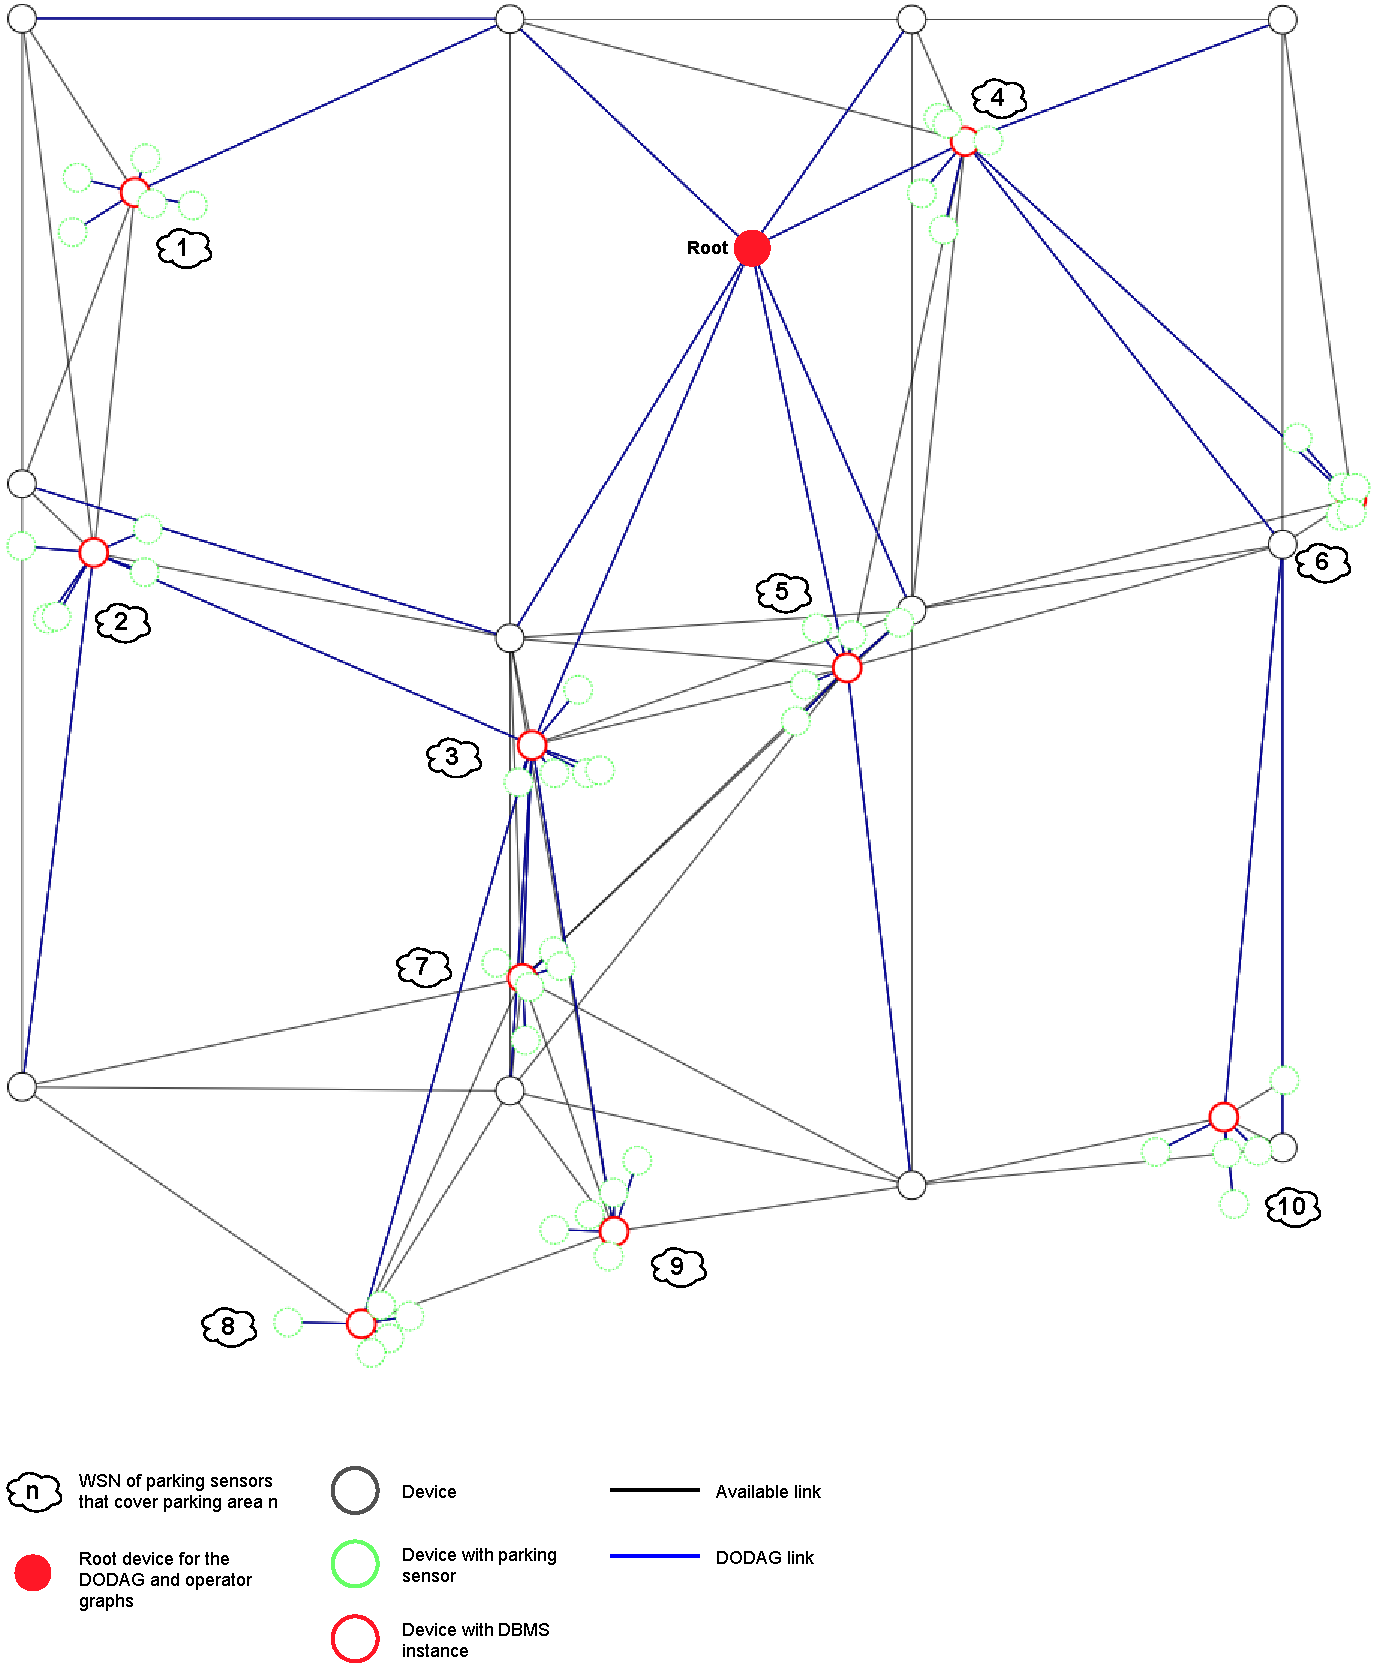
\includegraphics[scale=0.6]{figure_evaluation_visualization.pdf}
  \caption{Visualization of the finished topology of the example scenario including the DODAG}
  \label{figure_evaluation_visualization}
\end{figure}

Figure~\ref{figure_evaluation_visualization} shows the visualization of the finished topology for the distributed case. In the centralized case, only the fog node is a DBMS node, otherwise the topology is identical. The grid of the mesh topology is clearly visible in the figure. The top left node is the starting node of the mesh topology. Starting from this node, the network has up to $460m$ signal coverage in the south and up to $560m$ in the east. The signal range of the devices is configured with $200m$ so that fewer devices have to be simulated. In addition, only $5$ parking spaces are modeled for each parking area. RPL uses the hop count for the rank calculation.

To carry out the experiment, the two configuration files for the centralized and the distributed case are executed for each SPARQL query. During execution, each sensor sends a total of 10 samples to its data sink. Then the SPARQL query is sent once to the fog node.


\subsection{Experiment Results}
The results are shown in Table~\ref{table_evaluation_query}. The total number of packets sent and the network traffic caused by these packets are compared between the centralized and the distributed case. A sent packet travels from the source to the destination along the route in the DODAG. Several hops may be visited in the process. Packets sent by the hops are not counted. The measurement of the network traffic takes into account all links between source and destination including the links between the hops.
\begin{table}[htpb]

  \centering
    \begin{tabular}{c|cc|cc}
    \multicolumn{1}{c}{} & \multicolumn{2}{c}{\uzlemph{Centralized Case}} & \multicolumn{2}{c}{\uzlemph{Distributed Case}}\\
    & Sent Packages & Kilobytes Traffic & Sent Packages & Kilobytes Traffic
    \\ \uzlhline
    Only Sample Inserts & 500 & 724 & 29060 & 9330\\[3ex]
    Listing~\ref{appendix_query_1} & 500 & 724 & 29080 & 9451\\[3ex]
    Listing~\ref{appendix_query_2} & 500 & 724 & 29080 & 9384\\[3ex]
    Listing~\ref{appendix_query_3} & 500 & 724 & 29132 & 9459\\[3ex]
    Listing~\ref{appendix_query_4} & 500 & 724 & 29080 & 9431\\[3ex]
    Listing~\ref{appendix_query_5} & 500 & 724 & 29118 & 9413\\[3ex]
    Listing~\ref{appendix_query_6} & 500 & 724 & 29216 & 9737\\[3ex]
    Listing~\ref{appendix_query_7} & 500 & 724 & 29216 & 9761\\[3ex]
    Listing~\ref{sparql_query_usecase} & 500 & 724 & 29216 & 9726
    \end{tabular}
    \caption{Comparison between the centralized and distributed case in the experimental scenario.\label{table_evaluation_query}}
\end{table}

The result data from the centralized case is expected to be all the same. With $5$ sensors per WSN, each sending $10$ samples, this results in a total of $500$ sample packages. The traffic is $724$ kilobytes because there are several links between the sensor and the fog node. The payload of a sample package is $474$ bytes. This is the byte array size of the SPARQL insert query from Listing~\ref{appendix_query_insert}. The strings in the payloads of the sent DBMS packets are also measured uncompressed with their byte array size.

The result data in the distributed case is far too high. The reason for this can be seen in the first row of the table. In the first simulation run, only sample packets are sent and there is no subsequent query. The $500$ sensor samples cause $29060$ packets (sample packets and DBMS  packets) to be sent in the distributed case. The current implementation in LUPOSDATE3000 distributes the sample data over all existing instances. Compared to the centralized case, the distributed case is clearly worse. The next rows of the table show the results of simulation runs in which a query is also sent after the $500$ sensor samples. The number of packets for query processing is obtained by subtracting the number of packets from the first line. For example, processing the query in Listing~\ref{appendix_query_1} only results in $29080 - 29060 = 20$ packets.

The problem seems to be the distribution of the sensor data. A new experiment is carried out to clarify the problem. This time there is only one sensor and only one sample is taken. The fog node has this sensor and is therefore a data source and data sink at the same time. Another DBMS node is added in each subsequent simulation run. The locations and number of added nodes are based on the example scenario. This enables us to determine the overhead caused for different degrees of distribution in DBMS instances. The result of the experiment is shown in Figure~\ref{figure_evaluation_sampling_distribute}. With $11$ DBMS instances, $66$ packets are already sent for only one parking sample.
\begin{figure}[htpb]
  \centering
  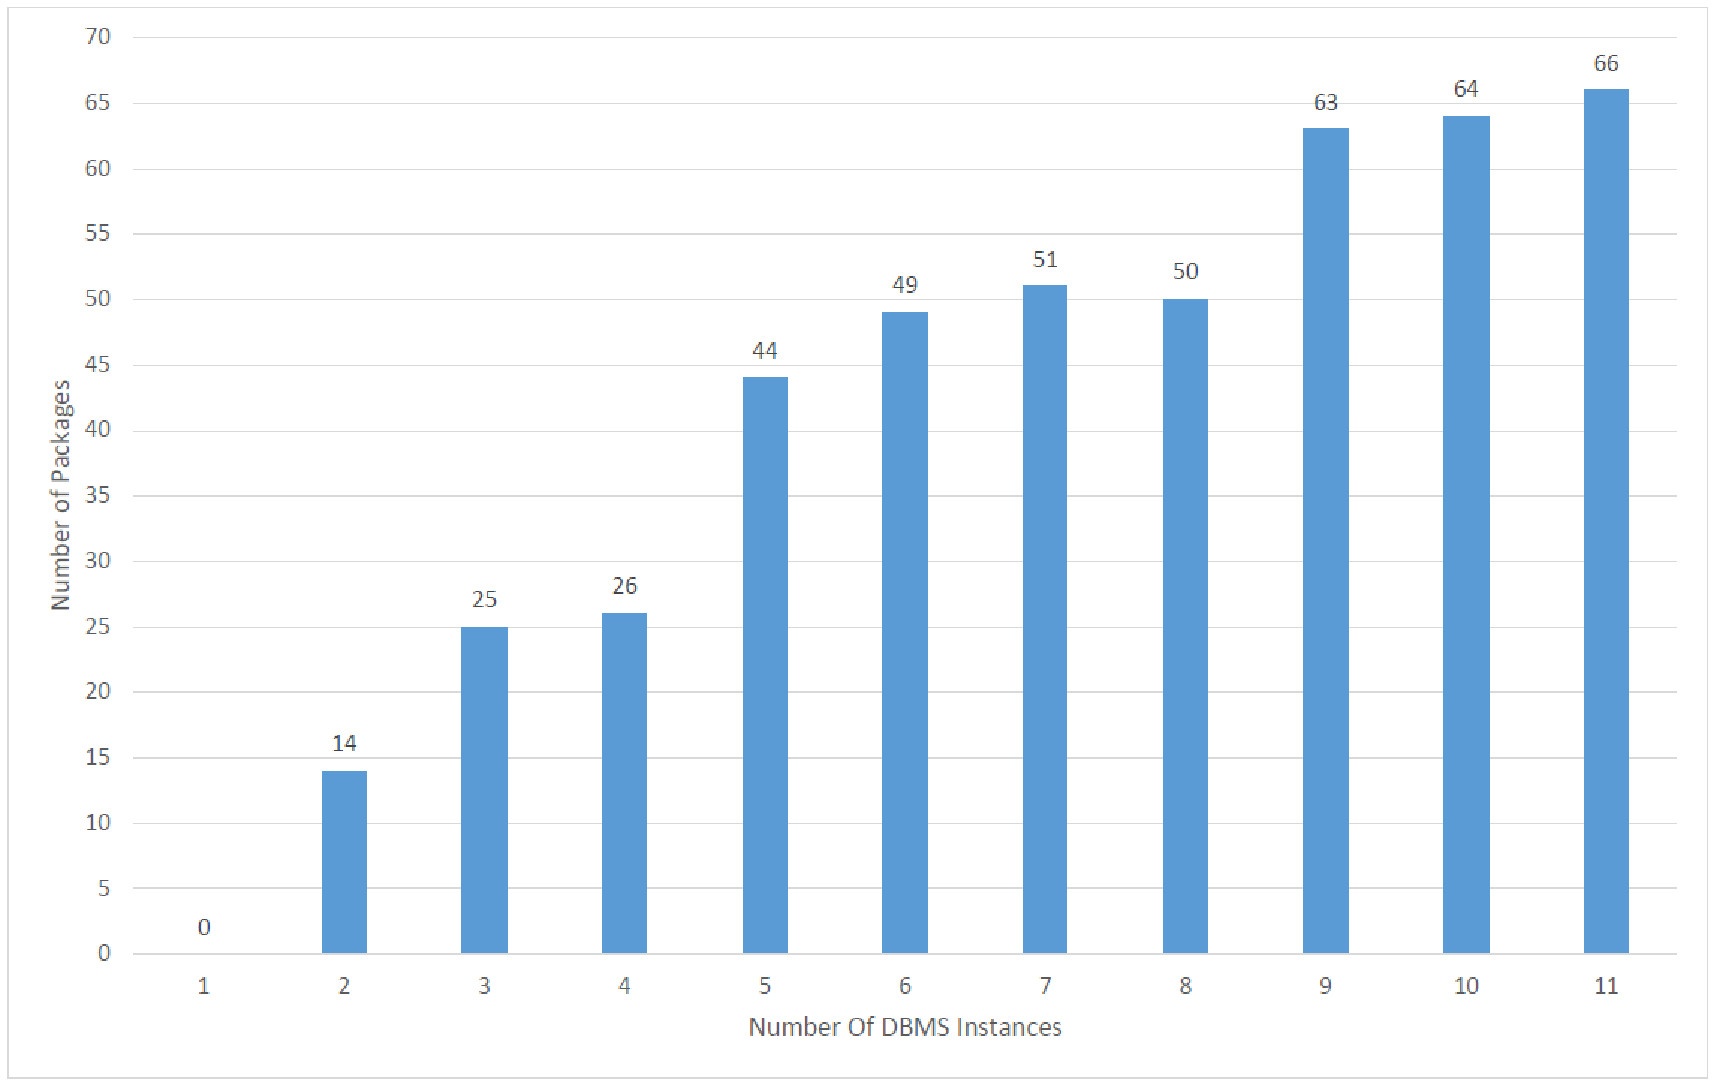
\includegraphics[scale=0.5]{figure_evaluation_sampling_distribute.pdf}
  \caption{11 DBMS instances already cause 66 messages with only one sample.\label{figure_evaluation_sampling_distribute}}
  
\end{figure}

In a further experiment, only the number of samples is increased and the topology already includes the $11$ DBMS instances. The sensor of the fog node collects an additional sample with each subsequent simulation run. Figure~\ref{figure_evaluation_sampling_number} shows the increase in number of packets sent. These result data lead to the conclusion that in the current implementation of LUPOSDATE3000 the overhead of the sensor data distribution is also dependent on the number of data sinks. Compared to the data from the distributed case in Table~\ref{table_evaluation_query}, where the samples are sent to $10$ different data sinks, the number of packets is $29060 - 27830 = 1230$ less if there is only one data sink.
\begin{figure}[htpb]
  \centering
  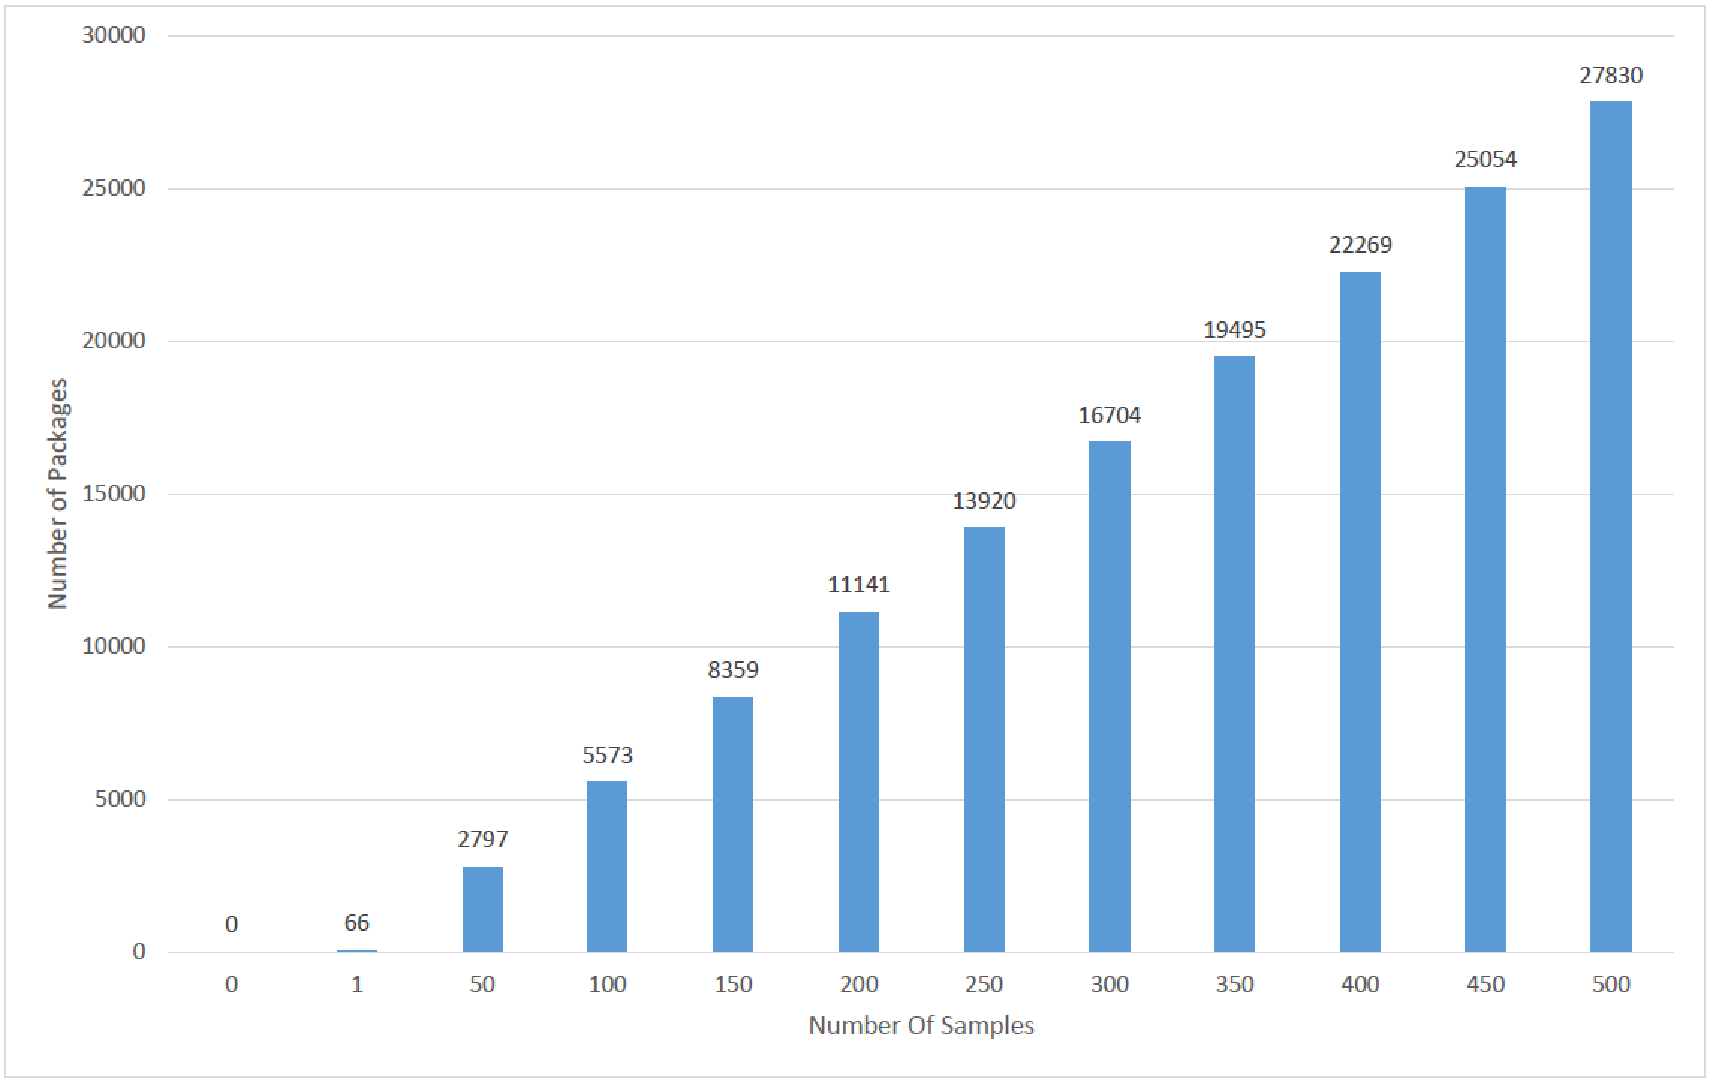
\includegraphics[scale=0.5]{figure_evaluation_sampling_number.pdf}
  \caption{Shows how the increasing number of samples increases the number of packages.\label{figure_evaluation_sampling_number}}
  
\end{figure}

\subsection{Experiment Conclusion}
Due to the current implementation of the sensor data distribution, the distributed case causes a considerable overhead with regard to the number of packets and network load. However, if the sensor data were not distributed across all instances, the distributed case could possibly perform better than the first case. To test this hypothesis, an additional experiment is carried out in which the sensor data is not distributed. In the configuration file of the distributed case, the LUPOSDATE3000 instances are exchanged with the dummy DBMS. The dummy DBMS does not distribute the data, nor is query processing performed. It is only a placeholder for a real DBMS. We use this experiment to find out the maximum overhead that the distributed query processing can have in order to perform better than in the centralized case.
The experimental result data in Table~\ref{table_evaluation_query_dummy} show that distributed query processing can have a maximum of $724 - 258 = 466$ kilobytes of traffic.
\begin{table}[htpb]
  \centering
    \begin{tabular}{c|cc|cc}
    \multicolumn{1}{c}{} & \multicolumn{2}{c}{\uzlemph{Centralized Case}} & \multicolumn{2}{c}{\uzlemph{Distributed Case (Dummy)}}\\
    & Sent Packages & Kilobytes Traffic & Sent Packages & Kilobytes Traffic
    \\ \uzlhline
    Only Sample Inserts & 500 & 724 & 500 & 258
    \end{tabular}
    \caption{The dummy DBMS shows how much network traffic should be caused by the parking samples in the distributed case.\label{table_evaluation_query_dummy}}
\end{table}

In the next step, the currently caused overhead of the distributed query processing is calculated. The results for each query are shown in Table~\ref{table_evaluation_query_calc}. The numbers are obtained by subtracting the numbers from the first row of the table. The query processing traffic is always less than $466$ kilobytes. This fact gives an indication that the distributed case without sensor data distribution can be more resource efficient than the centralized case. However, it remains only an indication, because the query processing also works differently without sensor data distribution.
\begin{table}[htpb]
  \centering
    \begin{tabular}{c|cc|cc}
    \multicolumn{1}{c}{} & \multicolumn{4}{c}{\uzlemph{Distributed Case}} \\
    \multicolumn{1}{c}{} & \multicolumn{2}{c}{\uzlemph{Total}} & \multicolumn{2}{c}{\uzlemph{Query Processing}}\\
    & Sent Packages & Kilobytes Traffic & Sent Packages & Kilobytes Traffic
    \\ \uzlhline
    Only Sample Inserts & 29060 & 9330 & 0 & 0\\[3ex]
    Listing~\ref{appendix_query_1} & 29080 & 9451 & 20 & 121\\[3ex]
    Listing~\ref{appendix_query_2} & 29080 & 9384 & 20 & 54\\[3ex]
    Listing~\ref{appendix_query_3} & 29132 & 9459 & 72 & 129\\[3ex]
    Listing~\ref{appendix_query_4} & 29080 & 9431 & 20 & 101\\[3ex]
    Listing~\ref{appendix_query_5} & 29118 & 9413 & 58 & 83\\[3ex]
    Listing~\ref{appendix_query_6} & 29216 & 9737 & 156 & 407\\[3ex]
    Listing~\ref{appendix_query_7} & 29216 & 9761 & 156 & 431\\[3ex]
    Listing~\ref{sparql_query_usecase} & 29216 & 9726 & 156 & 396
    \end{tabular}
    \caption{Shows the overhead due to distributed query processing.\label{table_evaluation_query_calc}}
\end{table}




\chapter{Conclusion}
\label{chapter_Conclusion}
The edge computing paradigm offers new possibilities to develop latency-sensitive and highly scalable IoT applications. The software components of the application can be deployed on smart devices at the edge of the Internet in the immediate vicinity of the data source. However, the development of such systems is challenging because the infrastructure has to be available.

In this master's thesis we present a new simulator to support the development of such systems in the edge computing environment. Existing systems can be connected via an interface and tested in any configurable environment. The focus of this simulator is on distributed DBMS. The modeled instances can be run on Fog and Edge nodes. The usefulness of the simulator is checked with the distributed Semantic Web DBMS LUPOSDATE3000. A performance analysis showed how many nodes can be simulated with and without this DBMS.

The second part of this master's thesis is the design of a protocol for distributed query processing in edge computing. The query processing uses an IoT routing protocol such as RPL to map the operators from the operator graph to existing DBMS nodes in the routing tree in a decentralized and dynamic manner. Several options for implementing the protocol were discussed. Ultimately, a universal protocol description was presented. The protocol implementation in LUPOSDATE3000 is evaluated with the simulator in an example scenario. The comparison between the centralized and the distributed case showed that the current sensor data distribution strategy in LUPOSDATE3000 is not optimal.

\subsection{Future Work}
\begin{itemize}
 \item The most important next step in the further development of LUPOSDATE3000 is to design a more resource-efficient sensor data distribution strategy. Sensor data should be stored at the edge of the network in the data sink or at least in the vicinity of the data sink. By limiting the data to a few instances for data storage, a distinction can also be made between data storage and query processing. The evaluation can then be repeated with the cases defined in Chapter~\ref{chapter_Concept} in order to obtain further results.
 \item In order to create more test cases, the RDF data from the example scenario can be supplemented with additional variables. Ideas for new variables in the context of the Parking Space Finder scenario can be found in~\cite{parkingJson}. In addition to the dynamically generated sensor data, static data can also be stored in advance in the DBMS instances. This combination of static and dynamic data in one scenario is more realistic.
 \item Another step is to design a more efficient packet structure for transmission. A binary and compressed format will significantly improve the IoT suitability of distributed query processing. After redesigning the package structure, the evaluation results will be more accurate.
 \item In addition, an evaluation of the energy consumption is desirable because energy efficiency is an important criterion in the IoT. The number and size of packets is already a good indicator of energy consumption, but the nodes' sleep and active times have not yet been taken into account.
 \item It should also be evaluated whether and when there are frequently contacted nodes (hot spots) in the distributed query processing. If this is the case, strategies for an operator graph adapted to hot spots can be designed. 
 \item Furthermore, failures during query processing have not yet been taken into account. This is also an important topic because lossy networks are an integral part of the IoT. The protocol must specify the behavior in the event of topology changes. To take account of failures in the simulator, the RPL class must be expanded to include a DIO trickle timer. Acknowledge messages for DAOs and the implementation of DODAG repair mechanisms are necessary.
 \item The modeling of the execution time at a node based on the actual execution time on the simulation computer is suboptimal for an evaluation. It has been shown that simulation runs must be deterministic in order to obtain repeatable results. The execution time is also an important metric when determining energy consumption. Virtualization with containers, as it is already implemented in FogBed, may be helpful.
 \item Future work is also the implementation of distributed query processing with continuous queries. LUPOSDATE3000 will implement stream processing in the near future in order to be better adapted to the IoT platform. This simulator can serve as a test environment during development. Streams of sensor data can already be simulated. The order compliance of the packages is also implemented in the simulator.
\end{itemize}


 


\begin{bibtex-entries}

%INPROCEEDINGS

@inproceedings{AgriIoT,
    author      = {Andreas Kamilaris and Feng Gao and Francesc X. Prenafeta-Boldu\'{u} and Muhammad Intizar Ali},
    title       = {Agri-IoT: A Semantic Framework for Internet of Things-enabled Smart Farming Applications},
    booktitle   = {2016 IEEE 3rd World Forum on Internet of Things (WF-IoT)}, 
    year        = {2016},
    month       = {12},
    pages       = {442-447},
    url         = {https://doi.org/10.1109/WF-IoT.2016.7845467},
    publisher   = {IEEE},
    location    = {Reston, VA, USA},
}    
    
@inproceedings{HM3P,
    author      = {Sven Groppe and Jinghua Groppe},
    title       = {Hybrid Multi-Model Multi-Platform (HM3P) Databases},
    booktitle   = {9th International Conference on Data Science, Technology and Applications ({DATA})},
    year        = {2020},
    month       = {7},
    pages       = {177-184},
    url         = {https://doi.org/10.5220/0009802401770184},
    publisher   = {SciTePress},
    location    = {Online Streaming},
}

@inproceedings{CityBench,
    author      = {Muhammad Intizar Ali and Feng Gao and Alessandra Mileo},
    title       = {CityBench: A Configurable Benchmark to Evaluate RSP Engines Using Smart City Datasets},
    booktitle   = {The Semantic Web - ISWC 2015},
    year        = {2015},
    month       = {10},
    pages       = {374-389},
    url         = {https://doi.org/10.1007/978-3-319-25010-6_25},
    publisher   = {Springer},
    location    = {Bethlehem, PA, USA},
}

@inproceedings{FogComp,
    author      = {Bonomi, Flavio and Milito, Rodolfo and Zhu, Jiang and Addepalli, Sateesh},
    title       = {Fog Computing and Its Role in the Internet of Things},
    booktitle   = {Proceedings of the First Edition of the MCC Workshop on Mobile Cloud Computing},
    year        = {2012},
    month       = {8},
    pages       = {13-16},
    url         = {https://doi.org/10.1145/2342509.2342513},
    publisher   = {Association for Computing Machinery},
    location    = {Helsinki, Finland},
}

@inproceedings{FogAndCloud,
    author      = {M. {Yannuzzi} and R. {Milito} and R. {Serral-Gracià} and D. {Montero} and M. {Nemirovsky}},
    booktitle   = {19th International Workshop on Computer Aided Modeling and Design of Communication Links and Networks (CAMAD)},
    title       = {Key ingredients in an IoT recipe: Fog Computing, Cloud computing, and more Fog Computing},
    year        = {2014},
    month       = {12},
    pages       = {325-329},
    url         = {https://doi.org/10.1109/CAMAD.2014.7033259},
    publisher   = {IEEE},
    location    = {Athens, Greece},
}

@inproceedings{BuildValidModels,
    author      = {A. M. {Law}},
    booktitle   = {2008 Winter Simulation Conference (WSC)},
    title       = {How to build valid and credible simulation models},
    year        = {2008},
    month       = {12},
    pages       = {39-47},
    url         = {https://doi.org/10.1109/WSC.2008.4736054},
    publisher   = {IEEE},
    location    = {Miami, FL, USA},
}

@inproceedings{DiscreteEventSim,
    author      = {T. J. {Schriber} and D. T. {Brunner} and J. S. {Smith}},
    booktitle   = {2016 Winter Simulation Conference (WSC)},
    title       = {Inside discrete-event simulation software: How it works and why it matters},
    year        = {2016},
    month       = {12},
    pages       = {221-235},
    url         = {https://doi.org/10.1109/WSC.2016.7822091},
    publisher   = {IEEE},
    location    = {Washington, DC, USA},
}

@inproceedings{SimAccuracy,
    author      = {A. {Buss} and A. {Al Rowaei}},
    booktitle   = {2010 Winter Simulation Conference (WSC)},
    title       = {A comparison of the accuracy of discrete event and discrete time},
    year        = {2010},
    month       = {12},
    pages       = {1468-1477},
    url         = {https://doi.org/10.1109/WSC.2010.5679045},
    publisher   = {IEEE},
    location    = {Baltimore, MD, USA},
}

@inproceedings{smallWaist,
    author      = {Akhshabi, Saamer and Dovrolis, Constantine},
    booktitle   = {Proceedings of the ACM SIGCOMM 2011 Conference},
    title       = {The Evolution of Layered Protocol Stacks Leads to an Hourglass-Shaped Architecture},
    year        = {2011},
    month       = {8},
    pages       = {206-217},
    url         = {https://doi.org/10.1145/2018436.2018460},
    publisher   = {Association for Computing Machinery},    
    location    = {Toronto, Ontario, Canada},
}

@INPROCEEDINGS{DemystifyingFog,
  author        = {P. {Varshney} and Y. {Simmhan}},
  booktitle     = {IEEE 1st International Conference on Fog and Edge Computing (ICFEC)}, 
  title         = {Demystifying Fog Computing: Characterizing Architectures, Applications and Abstractions}, 
  year          = {2017},
  month         = {5},
  pages         = {115-124},
  url           = {https://doi.org/10.1109/ICFEC.2017.20},
  publisher     = {IEEE},
  location      = {Madrid, Spain},
}

@INPROCEEDINGS{RoutingIssuesSurvey,
  author        = {Amol Dhumane and Rajesh Prasad and Jayashree Prasad},
  booktitle     = {Proceedings of the International MultiConference of Engineers and Computer Scientists (IMECS)}, 
  title         = {Routing Issues in Internet of Things: A Survey}, 
  year          = {2016},
  month         = {3},
  pages         = {404-412},
  isbn          = {978-988-19253-8-1},
  publisher     = {Newswood Limited},
  location      = {Hong Kong, China},
}


@INPROCEEDINGS{Path2IoT,
    author={P. {Michalák} and P. {Watson}},
    booktitle={IEEE International Conference on Cloud Computing Technology and Science (CloudCom)},
    title={PATH2iot: A Holistic, Distributed Stream Processing System},
    year={2017},
    month = {12},
    publisher = {IEEE},
    pages={25-32},
    url={https://doi.org/10.1109/CloudCom.2017.35},
    location = {Hong Kong, China},
}

@inproceedings{ComparisonIoTPlatformArchitectures,
    author = {Guth, Jasmin and Breitenb{\"u}cher, Uwe and Falkenthal, Michael
    and Leymann, Frank and Reinfurt, Lukas},
    title = {Comparison of IoT Platform Architectures: A Field Study based on
    a Reference Architecture},
    booktitle = {2016 Cloudification of the Internet of Things (CIoT)},
    year = {2016},
    month = {11},
    pages = {1-6},
    url = {https://doi.org/10.1109/CIOT.2016.7872918},
    publisher = {IEEE},
    location = {Paris, France},
}

@inproceedings{Warnke21Flexible,
  author    = {Benjamin Warnke and Muhammad Waqas Rehan and Stefan Fischer and Sven Groppe},
  title     = {Flexible data partitioning schemes for parallel merge joins in semantic web queries},
  booktitle = {Datenbanksysteme f{\"u}r Business, Technologie und Web (BTW 2021)},
  series    = {Lecture Notes in Informatics (LNI)},
  volume    = {{P-311}},
  pages     = {237-256},
  publisher = {Gesellschaft f{\"u}r Informatik, Bonn},
  year      = {2021},
  url       = {https://doi.org/10.18420/btw2021-12},
  location =  {Dresden, Germany}
}

@inproceedings{Cougar,
  author    = {Philippe Bonnet and Johannes Gehrke and Praveen Seshadri},
  title     = {Towards Sensor Database Systems},
  booktitle = {International Conference on Mobile Data Management (MDM 2001)},
  series    = {Lecture Notes in Computer Science (LNCS)},
  volume    = {1987},
  pages     = {3-14},
  publisher = {Springer},
  year      = {2001},
  url       = {https://doi.org/10.1007/3-540-44498-X_1},
  location =  {Hong Kong, China}
}


@INPROCEEDINGS{WoT,
    author  = {Szilagyi, Ioan and Wira, Patrice},
    booktitle = {IECON 2016 - 42nd Annual Conference of the IEEE Industrial Electronics Society},
    title = {Ontologies and Semantic Web for the Internet of Things - a survey},
    year={2016},
    volume={},
    number={},
    pages={6949-6954},
    publisher     = {IEEE},
    month = {10},
    url = {https://doi.org/10.1109/IECON.2016.7793744},
    location =  {Florence, Italy},
}

@INPROCEEDINGS{RPLEndToEndEstimation,
    author =    {P. Pinto and A. Pinto and M. Ricardo},
    booktitle = {2013 IFIP Wireless Days (WD)}, 
    title =     {End-to-end delay estimation using RPL metrics in WSN}, 
    year =      {2013},
    month =     {11},
    volume={},
    number={},
    publisher     = {IEEE},
    pages =     {1-6},
    url =       {https://doi.org/10.1109/WD.2013.6686524},
    location =  {Valencia, Spain},
}

@INPROCEEDINGS{simulator_cooja,
  author =      {Osterlind, Fredrik and Dunkels, Adam and Eriksson, Joakim and Finne, Niclas and Voigt, Thiemo},
  booktitle =   {Proceedings. 2006 31st IEEE Conference on Local Computer Networks}, 
  title =       {Cross-Level Sensor Network Simulation with COOJA}, 
  year =        {2006},
  month =       {11},
  volume ={},
  number ={},
  pages =       {641-648},
  publisher     = {IEEE},
  url =         {https://doi.org/10.1109/LCN.2006.322172},
  location =    {Tampa, FL, USA},
  }
  
@inproceedings{OMNeT,
  title=    {An overview of the OMNeT++ simulation environment},
  author=   {Varga, Andr{\'a}s and Hornig, Rudolf},
  booktitle={Proceedings of the 1st International Conference on Simulation Tools and techniques for Communications, Networks and Systems \& workshops},
  isbn =    {978-963-9799-20-2},
  year  =   {2008},
  month =       {3},
  publisher     = {ICST},
  location =    {Marseille, France},
}

@inproceedings{simulator_MyiFogSim,
    author = {Lopes, M\'{a}rcio Moraes and Higashino, Wilson A. and Capretz, Miriam A.M. and Bittencourt, Luiz Fernando},
    booktitle= {UCC '17 Companion: Companion Proceedings of the10th International Conference on Utility and Cloud Computing},
    title = {MyiFogSim: A Simulator for Virtual Machine Migration in Fog Computing},
    year = {2017},
    month = {12},
    publisher = {Association for Computing Machinery},
    url = {https://doi.org/10.1145/3147234.3148101},
    pages = {47-52},
    location = {Austin, TX, USA},
}


@INPROCEEDINGS{simulator_CloudSimPlus,
  author={Silva Filho, Manoel C. and Oliveira, Raysa L. and Monteiro, Claudio C. and In\'acio, Pedro R. M. and Freire, M\'ario M.},
  booktitle={2017 IFIP/IEEE Symposium on Integrated Network and Service Management (IM)}, 
  title={CloudSim Plus: A Cloud Computing Simulation
Framework Pursuing Software Engineering
Principles for Improved Modularity, Extensibility
and Correctness}, 
  year={2017},
  month = {5},
  pages={400-406},
  url={https://doi.org/10.23919/INM.2017.7987304},
  publisher = {IEEE},
  location = {Lisbon, Portugal},
}


@INPROCEEDINGS{simulator_recap,
  author={Byrne, James and Svorobej, Sergej and Gourinovitch, Anna and Elango, Divyaa Manimaran and Liston, Paul and Byrne, P J and Lynn, Theo},
  booktitle={2017 Winter Simulation Conference (WSC)}, 
  title={RECAP simulator: Simulation of cloud/edge/fog computing scenarios}, 
  year={2017},
  month = {12},
  pages={4568-4569},
  url={https://doi.org/10.1109/WSC.2017.8248208},
  publisher = {IEEE},
  location = {Las Vegas, NV, USA},
}

@INPROCEEDINGS{simulator_SatEdgeSim,
  author={Wei, Junyong and Cao, Suzhi and Pan, Siyan and Han, Jiarong and Yan, Lei and Zhang, Lei},
  booktitle={2020 12th International Conference on Communication Software and Networks (ICCSN)}, 
  title={SatEdgeSim: A Toolkit for Modeling and Simulation of Performance Evaluation in Satellite Edge Computing Environments}, 
  year={2020},
  month = {6},
  pages={307-313},
  url={https://doi.org/10.1109/ICCSN49894.2020.9139057},
  publisher = {IEEE},
  location = {Chongqing, China},
}

@INPROCEEDINGS{simulator_FogBed,
  author={Coutinho, Antonio and Greve, Fabiola and Prazeres, Cassio and Cardoso, Joao},
  booktitle={2018 IEEE International Conference on Communications (ICC)}, 
  title={Fogbed: A Rapid-Prototyping Emulation Environment for Fog Computing}, 
  year={2018},
  month = {5},
  pages={1-7},
  url={https://doi.org/10.1109/ICC.2018.8423003},
  publisher = {IEEE},
  location = {Kansas City, MO, USA},
}

@INPROCEEDINGS{simulator_Mininet,
  author={R.L.S. {De Oliveira} and Ailton Akira Shinoda and Christiane Marie Schweitzer and Ligia Rodrigues Prete},
  booktitle={2014 IEEE Colombian Conference on Communications and Computing (COLCOM)}, 
  title={Using Mininet for emulation and prototyping Software-Defined Networks}, 
  year={2014},
  month = {6},
  pages={1-6},
  doi={https://doi.org/10.1109/ColComCon.2014.6860404},
  publisher = {IEEE},
  location = {Bogota, Colombia},
}


%ARTICLE


@article{InternetDesign,
    author = {Clark, D.},
    title = {The Design Philosophy of the DARPA Internet Protocols},
    year = {1988},
    month = {8},
    volume = {18},
    number = {4},
    url = {https://doi.org/10.1145/52325.52336},
    journal = {ACM SIGCOMM Computer Communication Review},
    pages = {106-114},
}

@article{SimOverview,
    author  = {Sergej Svorobej and Patricia Takako Endo and Malika Bendechache and Christos Filelis-Papadopoulos and Konstantinos M. Giannoutakis and George A. Gravvanis and Dimitrios Tzovaras and James Byrne and Theo Lynn},
    title   = {Simulating Fog and Edge Computing Scenarios: An Overview and Research Challenges},
    journal = {Future Internet},
    year    = {2019},
    month   = {2},
    volume  = {11},
    number  = {3},
    url     = {https://doi.org/10.3390/fi11030055},
}
    
@article{AnalyzeQualities,
    author  = {Majid Ashouri and Fabian Lorig and Paul Davidsson and Romina Spalazzese},
    title   = {Edge Computing Simulators for IoT System Design: An Analysis of Qualities and Metrics},
    journal = {Future Internet},
    year    = {2019},
    month   = {11},
    volume  = {11},
    number  = {11},
    url     = {https://doi.org/10.3390/fi11110235},
}
   
@article{IoTSim,
    author  = {Xuezhi Zeng and Saurabh Kumar Garg and Peter Strazdins and Prem Prakash Jayaraman and Dimitrios Georgakopoulos and Rajiv Ranjan},
    title   = {IOTSim: A simulator for analysing IoT applications},
    journal = {Journal of Systems Architecture},
    year    = {2017},
    month = {1},
    pages   = {93-107},
    volume  = {72},
    number  = {},
    url     = {https://doi.org/10.1016/j.sysarc.2016.06.008},
}  
%Number gibts nicht bei IOTSim
  
@article{BigDataSim,
    author  = {Rajiv Ranjan},
    title   = {Modeling and Simulation in Performance Optimization of Big Data Processing Frameworks}, 
    journal = {IEEE Cloud Computing},
    year    = {2014},
    month = {11},
    pages   = {14-19},
    volume  = {1},
    number  = {4},
    url     = {https://doi.org/10.1109/MCC.2014.84},
}  
 
@article{SimChallenges,
    author  = {Gabor Kecskemeti and Giuliano Casale and Devki Nandan Jha and Justin Lyon and Rajiv Ranjan},
    title   = {Modelling and Simulation Challenges in Internet of Things}, 
    journal = {IEEE Cloud Computing}, 
    year    = {2017},
    month = {3},
    pages   = {62-69},
    volume  = {4},
    number  = {1},
    url     = {https://doi.org/10.1109/MCC.2017.18},
} 
 
@article{SemanticModels,
    author  = {Richard Mietz and Sven Groppe and Kay Römer and Dennis Pfisterer},
    title   = {Semantic Models for Scalable Search in the Internet of Things}, 
    journal = {Journal of Sensor and Actuator Networks}, 
    year    = {2013},
    month = {3},
    pages   = {172-195},
    volume  = {2},
    number  = {2},
    url     = {https://doi.org/10.3390/jsan2020172},
} 
 
@article{Osmosis,
    author  = {Massimo Villari and Maria Fazio and Schahram Dustdar and Omer Rana and Devki Nandan Jha and Rajiv Ranjan},
    title   = {Osmosis: The Osmotic Computing Platform for Microelements in the Cloud, Edge, and Internet of Things}, 
    journal = {Computer}, 
    year    = {2019},
    month = {7},
    pages   = {14-26},
    volume  = {52},
    number  = {8},
    url     = {https://doi.org/10.1109/MC.2018.2888767},
}

@article{DewComp,
    author  = {Partha Pratim Ray},
    title   = {An Introduction to Dew Computing: Definition, Concept and Implications}, 
    journal = {IEEE Access}, 
    year    = {2017},
    month = {11},
    pages   = {723-737},
    volume  = {6},
    number  = {},
    url     = {https://doi.org/10.1109/ACCESS.2017.2775042},
}

    @Article{DefinitionDewComp,
        title     = {Definition and Categorization of Dew Computing},
        author    = {Yingwei Wang},
        journal   = {Open Journal of Cloud Computing (OJCC)},
        year      = {2016},
        volume    = {3},
        number    = {1},
        pages     = {1-7},
        url       = {http://nbn-resolving.de/urn:nbn:de:101:1-201705194546},
    }
  
@article{Farming,
    author  = {K. {Taylor} and C. {Griffith} and L. {Lefort} and R. {Gaire} and M. {Compton} and T. {Wark} and D. {Lamb} and G. {Falzon} and M. {Trotter}},
    journal = {IEEE Intelligent Systems},
    title   = {Farming the Web of Things},
    year    = {2013},
    month = {10},
    volume  = {28},
    number  = {6},
    pages   = {12-19},
    url     = {https://doi.org/10.1109/MIS.2013.102},
}

@article{TinyDB,
    author = {Madden, Samuel R. and Franklin, Michael J. and Hellerstein, Joseph M. and Hong, Wei},
    title = {TinyDB: An Acquisitional Query Processing System for Sensor Networks},
    year = {2005},
    month = {3},
    volume = {30},
    number = {1},
    url = {https://doi.org/10.1145/1061318.1061322},
    journal = {ACM Transactions on Database Systems},
    pages = {122-173},
}

@article{VendorLockIn,
    author = {Justice Opara-Martins and Reza Sahandi and Feng Tian},
    title = {Critical analysis of vendor lock-in and its impact on cloud computing migration: a business perspective},
    year = {2016},
    volume = {5},
    number = {4},
    url = {https://doi.org/10.1186/s13677-016-0054-z},
    journal = {Journal of Cloud Computing},
}


@article{RPLHybridMode,
    author = {Sukho Oh and DongYeop Hwang and Kangseok Kim and Ki-Hyung Kim},
    title = {A hybrid mode to enhance the downward route performance in routing protocol for low power and lossy networks},
    journal = {International Journal of Distributed Sensor Networks},
    volume = {14},
    number = {4},
    url = {https://doi.org/10.1177/1550147718772533},
    year = {2018}
}

@article{RPLApplications,
    author = {Sobral, José V. V. and Rodrigues, Joel J. P. C. and Rabêlo, Ricardo A. L. and Al-Muhtadi, Jalal and Korotaev, Valery},
    title = {Routing Protocols for Low Power and Lossy Networks in Internet of Things Applications},
    journal = {Sensors},
    volume = {19},
    number = {9},
    url = {https://doi.org/10.3390/s19092144},
    year = {2019}
}

@article{RPLMultiparent,
    author = {Iova, Oana and Theoleyre, Fabrice and Noël, Thomas},
    year = {2015},
    month = {02},
    pages = {},
    title = {Using Multiparent Routing in RPL to Increase the Stability and the Lifetime of the Network},
    volume = {29},
    journal = {Ad Hoc Networks},
    url = {https://doi.org/10.1016/j.adhoc.2015.01.020},
}

@article{WSNDatabases,
    author = {Abderrahmen Belfkih and Claude Duvallet and Bruno Sadeg},
    year = {2019},
    month = {11},
    pages = {4921-4946},
    title = {A survey on wireless sensor network databases},
    volume = {25},
    journal = {Wireless Networks},
    url = {https://doi.org/10.1007/s11276-019-02070-y},
}

@article{SNQP,
    title = {In-network wireless sensor network query processors: State of the art, challenges and future directions},
    journal = {Information Fusion},
    volume = {25},
    pages = {1-15},
    year = {2015},
    url = {https://doi.org/10.1016/j.inffus.2015.01.007},
    author = {Farhana Jabeen and Sarfraz Nawaz},
}

@article{DistributedDBS,
    author = {Bonifati, Angela and Chrysanthis, Panos K. and Ouksel, Aris M. and Sattler, Kai-Uwe},
    title = {Distributed Databases and Peer-to-Peer Databases: Past and Present},
    year = {2008},
    volume = {37},
    number = {1},
    url = {https://doi.org/10.1145/1374780.1374781},
    journal = {ACM SIGMOD Record},
    month = {3},
    pages = {5-11},
}

@article{TinyTurrent,
    title = {Decentralised Peer-to-Peer data dissemination in Wireless Sensor Networks},
    journal = {Pervasive and Mobile Computing},
    volume = {40},
    pages = {242-266},
    year = {2017},
    month = {9},
    url = {https://doi.org/10.1016/j.pmcj.2017.07.006},
    author = {Ricardo Simon Carbajo and Ciar\`{a}n Mc Goldrick},
}

@article{StreamDBSSurvey,
    title = {Distributed data stream processing and edge computing: A survey on resource elasticity and future directions},
    journal = {Journal of Network and Computer Applications},
    volume = {103},
    pages = {1-17},
    year = {2018},
    url = {https://doi.org/10.1016/j.jnca.2017.12.001},
    author = {Marcos {Dias de Assun\c{c}\H{a}o} and Alexandre {da Silva Veith} and Rajkumar Buyya},
}

@article{SWPaper,
    urldate =  {2021-06-04},
    URL = {http://www.jstor.org/stable/26059207},
    author = {Tim Berners-Lee and James Hendler and Ora Lassila},
    journal = {Scientific American},
    number = {5},
    pages = {34-43},
    title = {The Semantic Web},
    volume = {284},
    year = {2001}
}

@article{MIPS,
    author = {Jongwon Lee and Jaejun Ko and Young-June Choi},
    title ={Dhrystone million instructions per second-based task offloading from smartwatch to smartphone},
    journal = {International Journal of Distributed Sensor Networks},
    volume = {13},
    number = {11},
    year = {2017},
    url = {https://doi.org/10.1177/1550147717740073},
}

@ARTICLE{FogNetSim,
  author={Qayyum, Tariq and Malik, Asad Waqar and Khan Khattak, Muazzam A. and Khalid, Osman and Khan, Samee U.},
  journal={IEEE Access}, 
  title={FogNetSim++: A Toolkit for Modeling and Simulation of Distributed Fog Environment}, 
  year={2018},
  volume={6},
  number={},
  pages={63570-63583},
  url={https://doi.org/10.1109/ACCESS.2018.2877696},
  }


@article{IoTSimEdge,
    author = {Jha, Devki Nandan and Alwasel, Khaled and Alshoshan, Areeb and Huang, Xianghua and Naha, Ranesh Kumar and Battula, Sudheer Kumar and Garg, Saurabh and Puthal, Deepak and James, Philip and Zomaya, Albert and Dustdar, Schahram and Ranjan, Rajiv},
    title = {IoTSim-Edge: A simulation framework for modeling the behavior of Internet of Things and edge computing environments},
    journal = {Software: Practice and Experience},
    volume = {50},
    number = {6},
    pages = {844-867},
    url = {https://doi.org/10.1002/spe.2787},
    year = {2020}
}
  
  
@article{simulator_CloudSim,
    author = {Calheiros, Rodrigo N. and Ranjan, Rajiv and Beloglazov, Anton and De Rose, C\'{e}sar A. F. and Buyya, Rajkumar},
    title = {CloudSim: a toolkit for modeling and simulation of cloud computing environments and evaluation of resource provisioning algorithms},
    journal = {Software: Practice and Experience},
    volume = {41},
    number = {1},
    pages = {23-50},
    url = {https://doi.org/10.1002/spe.995},
    year = {2011}
}

@article{simulator_EdgeCloudSim,
    author = {Sonmez, Cagatay and Ozgovde, Atay and Ersoy, Cem},
    title = {EdgeCloudSim: An environment for performance evaluation of edge computing systems},
    journal = {Transactions on Emerging Telecommunications Technologies},
    volume = {29},
    number = {11},
    url = {https://doi.org/10.1002/ett.3493},
    year = {2018}
}

@article{simulator_osmosis,
    title = {IoTSim-Osmosis: A framework for modeling and simulating IoT applications over an edge-cloud continuum},
    journal = {Journal of Systems Architecture},
    volume = {116},
    pages = {101956},
    year = {2021},
    issn = {1383-7621},
    url = {https://doi.org/10.1016/j.sysarc.2020.101956},
    author = {Khaled Alwasel and Devki Nandan Jha and Fawzy Habeeb and Umit Demirbaga and Omer Rana and Thar Baker and Scharam Dustdar and Massimo Villari and Philip James and Ellis Solaiman and Rajiv Ranjan},
}


@article{simulator_iFogSim,
    author = {Gupta, Harshit and Vahid Dastjerdi, Amir and Ghosh, Soumya K. and Buyya, Rajkumar},
    title = {iFogSim: A toolkit for modeling and simulation of resource management techniques in the Internet of Things, Edge and Fog computing environments},
    journal = {Software: Practice and Experience},
    volume = {47},
    number = {9},
    pages = {1275-1296},
    url = {https://doi.org/10.1002/spe.2509},
    year = {2017}
}

@article{simulator_PureEdgeSim,
    author = {Mechalikh Charafeddine and Taktak Hajer and Moussa Faouzi},
    title = {PureEdgeSim: A simulation framework for performance evaluation of cloud, edge and mist computing environments},
    journal = {Computer Science and Information Systems},
    volume = {18},
    number = {1},
    pages = {43-66},
    url = {https://doi.org/10.2298/CSIS200301042M},
    year = {2021}
}

@ARTICLE{simulator_YAFS,
  author={Lera, Isaac and Guerrero, Carlos and Juiz, Carlos},
  journal={IEEE Access}, 
  title={YAFS: A Simulator for IoT Scenarios in Fog Computing}, 
  year={2019},
  volume={7},
  number={},
  pages={91745-91758},
  url={https://doi.org/10.1109/ACCESS.2019.2927895},
}

@article{routingSurvey,
	author = {Hanumat Prasad Alahari and Suresh Babu Yalavarthi},
	title = {A Survey on Network Routing Protocols in Internet of Things (IOT)},
	journal = {International Journal of Computer Applications},
	volume = {160},
	number = {2},
	month = {2},
	year = {2017},
	pages = {18-22},
	url = {https://doi.org/10.5120/ijca2017912973},
}

    @Article{parkingJson,
        title     = {ParkingJSON: An Open Standard Format for Parking Data in Smart Cities},
        author    = {Gowri Sankar Ramachandran and
                     Jeremy Stout and
                     Joyce J. Edson and
                     Bhaskar Krishnamachari},
        journal   = {Open Journal of Internet Of Things (OJIOT)},
        issn      = {2364-7108},
        year      = {2020},
        volume    = {6},
        number    = {1},
        pages     = {105--118},
        url       = {http://nbn-resolving.de/urn:nbn:de:101:1-2020080219342154738409},
        urldate =      {2021-07-26},
        publisher = {RonPub},
    }
  

@incollection{BENSKY,
    title = {Chapter 12 - Wireless personal area networks},
    editor = {Alan Bensky},
    booktitle = {Short-range Wireless Communication (Third Edition)},
    publisher = {Newnes},
    edition = {Third Edition},
    pages = {317-360},
    year = {2019},
    isbn = {978-0-12-815405-2},
    url = {https://doi.org/10.1016/B978-0-12-815405-2.00012-9},
    author = {Alan Bensky},
}

   
% TECHREPORT    

@TechReport{FogCompConc,
  author =       {Michaela Iorga and Larry Feldman and Robert Barton and Michael J. Martin and Nedim Goren and Charif Mahmoudi},
  title =        {Fog Computing Conceptual Model},
  institution =  {National Institute of Standards and Technology, The University of Melbourne},
  year =         {2018},
  month =        {3},
  url =          {https://doi.org/10.6028/NIST.SP.500-325},
  number =       {500-325},
  address =      {Gaithersburg, MD, USA},
}

@TechReport{IoTEvolution,
  author =       {Dave Evans},
  title =        {The Internet of Things: How the Next Evolution of the Internet Is Changing Everything},
  institution =  {Cisco IBSG},
  year =         {2011},
  month =        {4},
  url =          {https://www.cisco.com/c/dam/en_us/about/ac79/docs/innov/IoT_IBSG_0411FINAL.pdf},
  urldate =      {2021-03-10},
  type =         {White Paper},
}

@TechReport{RPLWhitepaper,
  author =       {JP Vasseur and Navneet Agarwal and Jonathan Hui and Zach Shelby and Paul Bertrand and Cedric Chauvenet},
  title =        {RPL: The IP routing protocol designed for low power and lossy networks},
  institution =  {Internet Protocol for Smart Objects (IPSO) Alliance},
  year =         {2011},
  month =        {4},
  url =          {http://www.cse.chalmers.se/edu/year/2016/course/DAT285B/PAPERS/rpl.pdf},
  urldate =      {2021-04-19},
  type =         {White Paper},
}

@techreport{rfc7228,
  author        = {C. Bormann and M. Ersue and A. Keranen},
  title         = {Terminology for Constrained-Node Networks},
  howpublished  = {Internet Requests for Comments},
  type          = {RFC},
  number        = {7228},
  year          = {2014},
  month         = {5},
  publisher     = {RFC Editor},
  institution   = {RFC Editor},
  url           = {https://tools.ietf.org/html/rfc7228},
}

@techreport{rfc4944,
  author        = {G. Montenegro and N. Kushalnagar and J. Hui and D. Culler},
  title         = {Transmission of IPv6 Packets over IEEE 802.15.4 Networks},
  howpublished  = {Internet Requests for Comments},
  type          = {RFC},
  number        = {4944},
  year          = {2007},
  month         = {10},
  publisher     = {RFC Editor},
  institution   = {RFC Editor},
  url           = {https://tools.ietf.org/html/rfc4944},
}

@techreport{rfc6550,
  author        = {T. Winter and P. Thubert and A. Brandt and J. Hui and R. Kelsey and P. Levis and K. Pister and R. Struik and JP. Vasseur and R. Alexander},
  title         = {RPL: IPv6 Routing Protocol for Low-Power and Lossy Networks},
  howpublished  = {Internet Requests for Comments},
  type          = {RFC},
  number        = {6550},
  year          = {2012},
  month         = {3},
  publisher     = {RFC Editor},
  institution   = {RFC Editor},
  url           = {https://tools.ietf.org/html/rfc6550},
}

@techreport{rfc6552,
  author        = {P. Thubert},
  title         = {Objective Function Zero for the Routing Protocol for Low-Power and Lossy Networks (RPL)},
  howpublished  = {Internet Requests for Comments},
  type          = {RFC},
  number        = {6552},
  year          = {2012},
  month         = {3},
  publisher     = {RFC Editor},
  institution   = {RFC Editor},
  url           = {https://tools.ietf.org/html/rfc6552},
}

@techreport{rfc7102,
  author        = {JP. Vasseur},
  title         = {Terms Used in Routing for Low-Power and Lossy Networks},
  howpublished  = {Internet Requests for Comments},
  type          = {RFC},
  number        = {7102},
  year          = {2014},
  month         = {1},
  publisher     = {RFC Editor},
  institution   = {RFC Editor},
  url           = {https://tools.ietf.org/html/rfc7102},
}

@techreport{rfc7252,
  author        = {Z. Shelby and K. Hartke and C. Bormann},
  title         = {The Constrained Application Protocol (CoAP)},
  howpublished  = {Internet Requests for Comments},
  type          = {RFC},
  number        = {7252},
  year          = {2014},
  month         = {6},
  publisher     = {RFC Editor},
  institution   = {RFC Editor},
  url           = {https://tools.ietf.org/html/rfc7252},
}

@techreport{SNasDB,
  author        = {Ramesh Govindan and Joseph M. Hellerstein and Wei Hong and Samuel Madden and Michael Franklin and Scott Shenker},
  title         = {The Sensor Network as a Database},
  number        = {02-771},
  year          = {2002},
  month         = {9},
  institution   = {Computer Science Department, University of Southern California},
}

@techreport{EuropeanCommission,
  author        = {{INFSO D.4 Networked Enterprise \& RFID INFSO G.2 Micro \& Nanosystems} and {RFID Working Group of the ETP (EPOSS)}},
  title         = {Internet of Things in 2020: Roadmap for the Future},
  year          = {2008},
  month         = {5},
  publisher     = {European Commission},
}

@techreport{StrategicRoadmap,
  author        = {Patrick Guillemin and Peter Friess},
  title         = {Internet of Things: Strategic Research Roadmap},
  year          = {2009},
  month         = {10},
  publisher     = {European Commission},
}

%BOOKS

@book{Weisberg,
    author    = {Michael Weisberg}, 
    title     = {Simulation and Similarity: Using Models to Understand the World},
    publisher = {Oxford University Press},
    year      = {2012},
    edition   = {Reprint},
    isbn      = {978-0190265120},
}

@book{BasisTest,
    author    = {Andreas Spillner and Tilo Linz and Hans Schaefer}, 
    title     = {Software Testing Foundations: A Study Guide for the Certified Tester Exam},
    publisher = {Rocky Nook},
    year      = {2014},
    edition   = {4},
    isbn      = {978-1937538422},
}

@book{SWBook,
    author    = {Sven Groppe}, 
    title     = {Data Management and Query Processing in Semantic Web Databases},
    publisher = {Springer},
    year      = {2011},
    isbn      = {978-3-642-19356-9},
}

@book{BookCisco,
    author    = {David Hanes and Gonzalo Salgueiro and Patrick Grossetete and Robert Barton and Jerome Henry}, 
    title     = {IoT Fundamentals: Networking Technologies, Protocols, and Use Cases for the Internet of Things },
    publisher = {Cisco Press},
    year      = {2017},
    edition   = {1},
    isbn      = {978-1-58714-456-1},
}

@book{Tanenbaum,
    author    = {Andrew S. Tanenbaum and David J. Wetherall}, 
    title     = {Computer Networks},
    publisher = {Pearson},
    year      = {2011},
    edition   = {5},
    isbn      = {978-0-13-255317-9},
}

@book{Schiller,
    author    = {Jochen Schiller}, 
    title     = {Mobile Communications},
    publisher = {Pearson},
    year      = {2003},
    edition   = {2},
    isbn      = {978-0-321-12381-7},
}

@book{Kurose,
    author    = {James F. Kurose and Keith W. Ross}, 
    title     = {Computer Networking: A Top Down Approach},
    publisher = {Pearson},
    year      = {2020},
    edition   = {8},
    isbn      = {9780135928523},
}

@book{Kemper,
    author    = {Alfons Kemper and Andr\`{e} Eickler}, 
    title     = {Datenbanksysteme: Eine Einf{\"u}hrung},
    publisher = {De Gruyter},
    year      = {2015},
    edition   = {10},
    isbn      = {978-3-11-044375-2},
}

@book{Rahm,
    author    = {Erhard Rahm}, 
    title     = {Mehrrechner-Datenbanksysteme: Grundlagen der verteilten und parallelen Datenbankverarbeitung},
    publisher = {Addison-Wesley},
    year      = {1994},
    edition   = {1},
    isbn      = {3-89319-702-8},
    note      = {URL: https://dbs.uni-leipzig.de/buecher/mrdbs},
}

@book{SWBookHitzler,
    author    = {Pascal Hitzler and Markus Kr{\"o}tzsch and Sebastian Rudolph and York Sure}, 
    title     = {Semantic Web: Grundlagen},
    publisher = {Springer},
    year      = {2008},
    edition   = {1},
    isbn      = {978-3-540-33993-9}
}



%Websites

@MISC{SimJavaTutorial,
  author       = {Costas Simatos},
  title        = {The SimJava Tutorial},
  year         = {2002},
  howpublished = {\url{http://www.dcs.ed.ac.uk/home/simjava/tutorial/}},
  note         = {(visited on 01/31/2021)}
}

@MISC{DTS,
  author       = {Cliff Zou},
  title        = {Chapter 8: Statistical Simulation, Discrete-Time Simulation},
  year         = {2013},
  howpublished = {\url{http://www.cs.ucf.edu/~czou/CDA6530-13/DiscreteTime-Simulation.pdf}},
  note         = {(visited on 01/31/2021)},
}

@MISC{TinyDBHomePage,
  author       = {Sam Madden},
  title        = {TinyDB: A Declarative Database for Sensor Networks},
  year         = {2003},
  howpublished = {\url{http://telegraph.cs.berkeley.edu/tinydb/history.htm}},
  note         = {(visited on 05/18/2021)},
}

@MISC{simulator_ns3,
  author       = {{ns-3 Consortium}},
  title        = {ns-3: Network Simulator},
  year         = {2021},
  howpublished = {\url{https://www.nsnam.org/}},
  note         = {(visited on 06/20/2021)},
}


@MISC{UML_Spec,
  author        = {{Object Management Group (OMG)}},
  title         = {Unified Modeling Language 2.5},
  howpublished =  {\url{https://www.omg.org/spec/UML/2.5/PDF}},
  year          = {2015},
  month         = {3},
  note         =  {(visited on 07/15/2021)},
}

@MISC{WorldPopulation,
  author        = {{United Nations}},
  title         = {World Population Prospects 2019},
  howpublished =  {\url{https://population.un.org/wpp/Download/Standard/Population/}},
  year          = {2019},
  note         =  {(visited on 07/19/2021)},
}


%Anderes

@unpublished{SpezModScript,
    author = {St{\"u}mpel, Annette},
    title = {Specification and Modeling, Institute for Software Engineering and Programming Languages, University of L{\"u}beck},
    note = {Unpublished university lecture notes},
    year = {2018},
}

@unpublished{AITScript,
    author = {Horst Hellbr{\"u}ck},
    title = {Advanced Internet Technologies, Institute of Telematics, University of L{\"u}beck},
    note = {Unpublished university lecture notes},
    year = {2019},
}


%THESIS

@mastersthesis{SimJavaThesis,
    author    = {Costas Simatos},
    title     = {Making SimJava Count},
    publisher = {The University of Edinburgh, School of Informatics},
    address   = {Edinburgh, Scotland, UK},
    year      = {2002},
}

@phdthesis{DissSimulation,
    author    = {Ahmed Ali Alrowaie},
    title     = {The Effect of Time-Advance Mechanism in Modeling And Simulation},
    publisher = {Naval Postgraduate School},
    address   = {Monterey, CA, USA},
    year      = {2011}
}

@phdthesis{AndreasTeubler,
    author    = {Andreas Teubler},
    title     = {Ein namenszentrischer Ansatz zur Realisierung von Diensten im Internet der Dinge},
    publisher = {University of L{\"u}beck},
    address   = {L{\"u}beck, Germany},
    year      = {2019},
    url       = {https://www.zhb.uni-luebeck.de/epubs/ediss2162.pdf},
    urldate   = {2021-05-25}
}


@Inbook{FogCloudBook,
    author="Mahmood, Zaigham
    and Ramachandran, Muthu",
    title="Fog Computing: Concepts, Principles and Related Paradigms",
    bookTitle="Fog Computing: Concepts, Frameworks and Technologies",
    year="2018",
    publisher="Springer International Publishing",
    pages="3--21",
    url="https://doi.org/10.1007/978-3-319-94890-4_1",
}


\end{bibtex-entries}

% If you need to have an appendix (I advise against it), insert it
% here using, first, \appendix and then \chapter and then,
% possibly, \section. 
%
% \appendix
%
% \chapter{Technical Appendix}
%
% \section{Experimental Parameters} % possibly
%

\appendix
\chapter{Queries for the Example Scenario}
\label{appendix_queries}

\begin{SPARQL}[caption={The samples are added with the $insert\; data$ operation.},
  float, label=appendix_query_insert, morekeywords={@prefix, insert, data}, captionpos=b]
@PREFIX rdf: <http://www.w3.org/1999/02/22-rdf-syntax-ns#> .
@PREFIX xsd: <http://www.w3.org/2001/XMLSchema#> .
@PREFIX sosa: <http://www.w3.org/ns/sosa/> .

INSERT DATA {
    <http://observation/1/sensor/9/2> rdf:type sosa:Observation ;
    sosa:hasFeatureOfInterest <http://parkingArea/9> ;
    sosa:observedProperty <http://parkingSpace/2> ;
    sosa:madeBySensor <http://sensor/9/2> ;
    sosa:hasSimpleResult "false"^^xsd:boolean ;
    sosa:resultTime "2021-06-09T15:41:01"^^xsd:dateTime .
}
\end{SPARQL}

\begin{SPARQL}[caption={Returns all triples.},
  float, label=appendix_query_1, morekeywords={@prefix}, captionpos=b]
SELECT ?s ?p ?o WHERE { ?s ?p ?o. }
\end{SPARQL}

\begin{SPARQL}[caption={Returns the number of parking areas.},
  float, label=appendix_query_2, morekeywords={@prefix}, captionpos=b]
PREFIX rdf: <http://www.w3.org/1999/02/22-rdf-syntax-ns#>
PREFIX xsd: <http://www.w3.org/2001/XMLSchema#>
PREFIX sosa: <http://www.w3.org/ns/sosa/>

select (count(distinct ?x) as ?count) 
where {
 ?s sosa:hasFeatureOfInterest ?x
}
\end{SPARQL}

\begin{SPARQL}[caption={Returns the number of parking spaces in area number 10. Assumption: Each parking space is observed by one sensor.},
  float, label=appendix_query_3, morekeywords={@prefix}, captionpos=b]
PREFIX rdf: <http://www.w3.org/1999/02/22-rdf-syntax-ns#>
PREFIX xsd: <http://www.w3.org/2001/XMLSchema#>
PREFIX sosa: <http://www.w3.org/ns/sosa/>

select  (count(distinct ?x) as ?count) 
where {
 ?b rdf:type sosa:Observation.
 ?b sosa:hasFeatureOfInterest  <http://parkingArea/10>.
 ?b sosa:madeBySensor ?x.   
}
\end{SPARQL}
\begin{SPARQL}[caption={Returns the number of samples from sensor number 67 from parking area number 9.},
  float, label=appendix_query_4, morekeywords={@prefix}, captionpos=b]
PREFIX rdf: <http://www.w3.org/1999/02/22-rdf-syntax-ns#>
PREFIX xsd: <http://www.w3.org/2001/XMLSchema#>
PREFIX sosa: <http://www.w3.org/ns/sosa/>

select (count(?b) as ?count) 
where {
 ?b rdf:type sosa:Observation.
 ?b sosa:madeBySensor <http://sensor/9/67>.   
}
\end{SPARQL}

\begin{SPARQL}[caption={Returns the latest sample of sensor number 55 from parking area number 7.},
  float, label=appendix_query_5, morekeywords={@prefix}, captionpos=b]
PREFIX rdf: <http://www.w3.org/1999/02/22-rdf-syntax-ns#>
PREFIX xsd: <http://www.w3.org/2001/XMLSchema#>
PREFIX sosa: <http://www.w3.org/ns/sosa/>

select (max(?d) AS ?latestdate)
where {
 ?b sosa:madeBySensor <http://sensor/7/55>.
 ?b sosa:resultTime ?d .
}
\end{SPARQL}

\begin{SPARQL}[caption={Returns the latest samples of all sensors from parking area number 9.},
  float, label=appendix_query_6, morekeywords={@prefix}, captionpos=b]
PREFIX rdf: <http://www.w3.org/1999/02/22-rdf-syntax-ns#>
PREFIX xsd: <http://www.w3.org/2001/XMLSchema#>
PREFIX sosa: <http://www.w3.org/ns/sosa/>

SELECT ?sensor ?isOccupied ?lastObservedAt
WHERE {
 ?o a sosa:Observation ;
 sosa:madeBySensor ?sensor;
 sosa:hasFeatureOfInterest <http://parkingArea/9>;
 sosa:hasSimpleResult ?isOccupied;
 sosa:resultTime ?lastObservedAt .
 {
   SELECT(MAX(?d) AS ?lastObservedAt) ?sensor WHERE{
     ?o2 a sosa:Observation ;
     sosa:madeBySensor ?sensor;
     sosa:hasFeatureOfInterest <http://parkingArea/9>;
     sosa:resultTime ?d .
   }
   GROUP BY ?sensor
 }
}
\end{SPARQL}

\begin{SPARQL}[caption={Returns the latest samples of all sensors from the parking areas number 9, number 8 and number 2.},
  float, label=appendix_query_7, morekeywords={@prefix}, captionpos=b]
PREFIX rdf: <http://www.w3.org/1999/02/22-rdf-syntax-ns#>
PREFIX xsd: <http://www.w3.org/2001/XMLSchema#>
PREFIX sosa: <http://www.w3.org/ns/sosa/>

SELECT ?sensor ?isOccupied ?lastObservedAt
WHERE {
 ?o a sosa:Observation ;
 sosa:madeBySensor ?sensor;
 sosa:hasFeatureOfInterest ?f;
 sosa:hasSimpleResult ?isOccupied;
 sosa:resultTime ?lastObservedAt .
 {
   SELECT(MAX(?d) AS ?lastObservedAt) ?sensor ?f WHERE{
     ?o2 a sosa:Observation ;
     sosa:madeBySensor ?sensor;
     sosa:hasFeatureOfInterest ?f;
     sosa:resultTime ?d .
     FILTER (?f IN (<http://parkingArea/9>, <http://parkingArea/8>, <http://parkingArea/2>))
   }
   GROUP BY ?sensor
 }
}
\end{SPARQL}

\end{document}

